\documentclass[twoside,11pt]{article}

% Any additional packages needed should be included after jmlr2e.
% Note that jmlr2e.sty includes epsfig, amssymb, natbib and graphicx,
% and defines many common macros, such as 'proof' and 'example'.
%
% It also sets the bibliographystyle to plainnat; for more information on
% natbib citation styles, see the natbib documentation, a copy of which
% is archived at http://www.jmlr.org/format/natbib.pdf

% Available options for package jmlr2e are:
%
%   - abbrvbib : use abbrvnat for the bibliography style
%   - nohyperref : do not load the hyperref package
%   - preprint : remove JMLR specific information from the template,
%         useful for example for posting to preprint servers.
%
% Example of using the package with custom options:
%
% \usepackage[abbrvbib, preprint]{jmlr2e}

\usepackage{bbm}
\usepackage{algorithmicx}
\usepackage{jmlr2e}
\usepackage{amsmath}
\usepackage{xcolor}
\usepackage{bm}
\usepackage{tikz}
\usetikzlibrary{bayesnet}
\usepackage{subcaption}
\usepackage{float}
\usepackage{stackengine}
\usepackage{minted}
\usepackage{array}
\usepackage{multirow}
\usepackage{stmaryrd}
\usepackage{pgfplots}
\usepgfplotslibrary{fillbetween}
\usetikzlibrary{patterns}
\usetikzlibrary{shapes.geometric}
\usepackage[ruled,vlined]{algorithm2e}
\usepackage{xstring}
\usepackage[margin=1cm,bottom=1in]{geometry}
\usepackage{xfp}

\definecolor{BlueCode}{RGB}{0,0,250}
\definecolor{GreenCode}{RGB}{0,125,0}

% Caligraphic font
\let\oldmathcal\mathcal
\DeclareMathAlphabet{\mathdutchcal}{U}{dutchcal}{m}{n}
\let\newmathcal\mathcal
\renewcommand{\mathcal}[1]{%
  \IfSubStr{ABCDEFGHIJKLMNOPQRSTUVWXYZ}{#1}{\oldmathcal{#1}}{\mathdutchcal{#1}}
}
\makeatother

% Definitions of handy macros can go here

\pgfmathdeclarefunction{gauss}{3}{%
  \pgfmathparse{1/(#3*sqrt(2*pi))*exp(-((#1-#2)^2)/(2*#3^2))}%
}
\pgfmathdeclarefunction{sum_gauss}{5}{%
  \pgfmathparse{1/(3*#3*sqrt(2*pi))*exp(-((#1-#2)^2)/(2*#3^2)) + 2/(3*#5*sqrt(2*pi))*exp(-((#1-#4)^2)/(2*#5^2))}%
}
\newcommand{\fracpartial}[2]{\frac{\partial #1}{\partial  #2}}
\newcommand{\kl}[2]{D_{\mathrm{KL}} \left[ \left. \left. #1 \right|\right| #2 \right] }
\DeclareMathOperator*{\argmax}{arg\,max}
\DeclareMathOperator*{\argmin}{arg\,min}
\definecolor{blue-violet}{rgb}{0.54, 0.17, 0.89}
\definecolor{bluepigment}{rgb}{0.2, 0.2, 0.6}
\makeatletter
\newcommand*\bigcdot{\mathpalette\bigcdot@{.5}}
\newcommand*\bigcdot@[2]{\mathbin{\vcenter{\hbox{\scalebox{#2}{$\m@th#1\bullet$}}}}}
\makeatother
\def\delequal{\mathrel{\ensurestackMath{\stackon[1pt]{=}{\scriptstyle\Delta}}}}
\definecolor{Yellow}{RGB}{211, 176, 15}
\definecolor{Green}{rgb}{0.01, 0.75, 0.24}
\colorlet{Red}{red!50!black}
\colorlet{Blue}{blue!50!black}
\definecolor{Violet}{rgb}{0.56,0.14,0.56}
\newcommand{\indep}{\perp \! \! \! \perp}
\newcommand{\MultiBernoulli}{\mathcal{B}\hspace{-0.02cm}\text{ernoulli}}



\makeatletter
\newcounter{subsubsubsection}[subsubsection]
\def\subsubsubsectionmark#1{}
\def\thesubsubsubsection {\thesubsubsection 
     .\arabic{subsubsubsection}}
\def\subsubsubsection{\@startsection
     {subsubsubsection}{4}{\z@} {-3.25ex plus -1
     ex minus -.2ex}{1.5ex plus .2ex}{\normalsize\bf}}
\def\l@subsubsubsection{\@dottedtocline{4}{4.8em}
     {4.2em}}
\makeatother


\tikzset{
    pics/vae/.style args={#1/#2/#3/#4/#5}{
    code = {
		\draw[fill=blue!20!white] (-1,-12) rectangle (1,-8);
	    \node at (0, -10) {#1};

		\coordinate (A) at (1.5,-12);
		\coordinate (B) at (4,-11);
		\coordinate (C) at (4,-9);
		\coordinate (D) at (1.5,-8);
		\draw[fill=green!20!white] (A) -- coordinate[pos=.6] (AB) (B)--(C)
         --coordinate[pos=.45] (CD) (D)
         --coordinate[pos=.55] (DA) cycle;
	    \node at (2.75, -10) {$Encoder$};

		\draw[fill=red!20!white] (4.5,-11) rectangle (5.5,-10.1);
	    \node at (5, -10.5) {#3};
		\draw[fill=red!20!white] (4.5,-9.9) rectangle (5.5,-9);
	    \node at (5, -9.5) {#2};

		\node[latent] at (5, -8.4) (epsilon) {$\epsilon$};

		\coordinate (A) at (7.5,-11);
		\coordinate (B) at (10,-12);
		\coordinate (C) at (10,-8);
		\coordinate (D) at (7.5,-9);
		\draw[fill=green!20!white] (A) -- coordinate[pos=.6] (AB) (B)--(C)
         --coordinate[pos=.45] (CD) (D)
         --coordinate[pos=.55] (DA) cycle;
	    \node at (8.75, -10) {$Decoder$};

		\draw[fill=gray!20!white] (6,-11) rectangle (7,-9);
	    \node at (6.5,-10) {#4};

		\draw[fill=blue!20!white] (10.5,-12) rectangle (12.5,-8);
	    \node at (11.5, -10) {#5};

		% arrows
		\draw[-latex] (4,-10.5) -- (4.5,-10.5);
		\draw[-latex] (4,-9.5) -- (4.5,-9.5);
		\draw[-latex] (1,-10) -- (1.5,-10);
		\draw[-latex] (5.36,-8.4) -- (5.75,-8.4) -- (5.75,-10) -- (6,-10);
		\draw[-latex] (5.5,-10.5) -- (5.75,-10.5) -- (5.75,-10) -- (6,-10);
		\draw[-latex] (5.5,-9.5) -- (5.75,-9.5) -- (5.75,-10) -- (6,-10);

		\draw[-latex] (7,-10) -- (7.5,-10);
		\draw[-latex] (10,-10) -- (10.5,-10);
    }}
}
    
\tikzset{
    pics/hmm/.code = {
    		\pic[rotate=90]{vae=$o_t$/$\mu$/$\ln \sigma$/$\hat{s}_t$/$\hat{o}_t$};

		\draw[fill=blue!20!white] (12,3.5) rectangle (13,5.5);
	    \node at (12.5, 4.5) {$a_t$};

		\coordinate (A) at (13.5,3.5);
		\coordinate (B) at (16,4.5);
		\coordinate (C) at (16,6.5);
		\coordinate (D) at (13.5,7.5);
		\draw[fill=orange!20!white] (A) -- coordinate[pos=.6] (AB) (B)--(C)
         --coordinate[pos=.45] (CD) (D)
         --coordinate[pos=.55] (DA) cycle;
	    \node at (14.75, 5.5) {$Transition$};

		\draw[fill=red!20!white] (16.5,4.5) rectangle (17.5,5.4);
	    \node at (17, 5) {$\ln \mathring{\sigma}$};
		\draw[fill=red!20!white] (16.5,5.6) rectangle (17.5,6.5);
	    \node at (17, 6) {$\mathring{\mu}$};
		\node[latent] at (17, 7.1) (epsilon) {$\epsilon$};

		\draw[fill=gray!20!white] (18,4.5) rectangle (19,6.5);
	    \node at (18.5, 5.5) {$\mathring{s}_{t+1}$};

		\draw[-latex] (13,4.5) -- (13.5,4.5);
		\draw[-latex] (11,6.5) -- (13.5,6.5);

		\draw[-latex] (16,5) -- (16.5,5);
		\draw[-latex] (16,6) -- (16.5,6);

		\draw[-latex] (17.5,6) -- (17.75,6) -- (17.75,5.5) -- (18,5.5);
		\draw[-latex] (17.5,5) -- (17.75,5) -- (17.75,5.5) -- (18,5.5);
		\draw[-latex] (17.36,7.1) -- (17.75,7.1) -- (17.75,5.5) -- (18,5.5);

		\pic[xshift=12cm,rotate=90]{vae=$o_{t+1}$/$\hat{\mu}$/$\ln \hat{\sigma}$/$\hat{s}_{t+1}$/$\hat{o}_{t+1}$};
    }
}

\tikzset{
    pics/fountas/.style args={#1/#2/#3/#4/#5}{
    code = {
		\draw[fill=blue!20!white] (-1,-12) rectangle (0,-8);
	    \node at (-0.5, -10) {#1};

		\coordinate (A) at (0.5,-12);
		\coordinate (B) at (3,-11);
		\coordinate (C) at (3,-9);
		\coordinate (D) at (0.5,-8);
		\draw[fill=green!20!white] (A) -- coordinate[pos=.6] (AB) (B)--(C)
         --coordinate[pos=.45] (CD) (D)
         --coordinate[pos=.55] (DA) cycle;
	    \node at (1.75, -10) {$Encoder$};

		\draw[fill=red!20!white] (3.5,-11) rectangle (4.5,-10.1);
	    \node at (4, -10.5) {#3};
		\draw[fill=red!20!white] (3.5,-9.9) rectangle (4.5,-9);
	    \node at (4, -9.5) {#2};

		\node[latent] at (4, -8.4) (epsilon) {$\epsilon$};

		\coordinate (A) at (8,-4);
		\coordinate (B) at (10.5,-5);
		\coordinate (C) at (10.5,-1);
		\coordinate (D) at (8,-2);
		\draw[fill=green!20!white] (A) -- coordinate[pos=.6] (AB) (B)--(C)
         --coordinate[pos=.45] (CD) (D)
         --coordinate[pos=.55] (DA) cycle;
	    \node at (9.25, -3) {$Decoder$};

		\draw[fill=gray!20!white] (5,-11) rectangle (6,-9);
	    \node at (5.5,-10) {#4};

		\draw[fill=blue!20!white] (7,-11) rectangle (8,-9);
	    \node at (7.5, -10) {$a_t$};

		\draw[fill=blue!20!white] (11,-5) rectangle (12,-1);
	    \node at (11.5, -3) {#5};

		\draw[-latex] (7.5,-3) -- (8,-3);
		\draw[-latex] (10.5,-3) -- (11,-3);

		% arrows
		\draw[-latex] (3,-10.5) -- (3.5,-10.5);
		\draw[-latex] (3,-9.5) -- (3.5,-9.5);
		\draw[-latex] (0,-10) -- (0.5,-10);
		\draw[-latex] (4.36,-8.4) -- (4.75,-8.4) -- (4.75,-10) -- (5,-10);
		\draw[-latex] (4.5,-10.5) -- (4.75,-10.5) -- (4.75,-10) -- (5,-10);
		\draw[-latex] (4.5,-9.5) -- (4.75,-9.5) -- (4.75,-10) -- (5,-10);
		
		\coordinate (A) at (4.5,-8);
		\coordinate (B) at (5.5,-5.5);
		\coordinate (C) at (7.5,-5.5);
		\coordinate (D) at (8.5,-8);
		\draw[fill=orange!20!white] (A) -- coordinate[pos=.6] (AB) (B)--(C)
         --coordinate[pos=.45] (CD) (D)
         --coordinate[pos=.55] (DA) cycle;
	    \node at (6.5, -6.75) {$Transition$};
		
		\draw[-latex] (5.95,-5.5) -- (5.95,-5);
		\draw[-latex] (7.05,-5.5) -- (7.05,-5);

		\draw[-latex] (5.95,-4) -- (5.95,-3.75) -- (6.5,-3.75) -- (6.5,-3.5);
		\draw[-latex] (7.05,-4) -- (7.05,-3.75) -- (6.5,-3.75) -- (6.5,-3.5);
		\draw[-latex] (4.9,-4.1) -- (4.9,-3.75) -- (6.5,-3.75) -- (6.5,-3.5);

		\draw[-latex] (5.5,-9) -- (5.5,-8);
		\draw[-latex] (7.5,-9) -- (7.5,-8);

		\draw[fill=red!20!white] (5.5,-5) rectangle (6.4,-4);
	    \node at (5.95,-4.5) {$\mathring{\mu}$};
		\draw[fill=red!20!white] (6.6,-5) rectangle (7.5,-4);
	    \node at (7.05,-4.5) {$\ln \mathring{\sigma}$};
		\node[latent] at (4.9,-4.5) (epsilon) {$\epsilon$};

		\draw[fill=gray!20!white] (5.5,-3.5) rectangle (7.5,-2.5);
	    \node at (6.5, -3) {$\mathring{s}^r_{t+1}$};
    }}
}

\tikzset{
    pics/dense/.style args={#1/#2/#3/#4}{
    code = {
    		\draw[fill=green!30!white] (\fpeval{#1-1.75},\fpeval{#2-0.25}) rectangle (\fpeval{#1+1.75},\fpeval{#2+0.75});
		\node[rotate=90] at (\fpeval{#1-1.95},\fpeval{#2+0.25}) {#4};
		\node at (#1,#2+0.25) {\textbf{size:} #3};
    }}
}

\tikzset{
    pics/dropout/.style args={#1/#2/#3}{
    code = {
    		\draw[fill=blue!30!white] (\fpeval{#1-1.75},\fpeval{#2-0.25}) rectangle (\fpeval{#1+1.75},\fpeval{#2+0.75});
		\node at (#1,#2+0.25) {\textbf{rate:} #3};
    }}
}

\tikzset{
    pics/upconv/.style args={#1/#2/#3/#4/#5/#6}{
    code = {
    		\draw[fill=yellow!30!white] (\fpeval{#1-1.75},\fpeval{#2-0.75}) rectangle (\fpeval{#1+1.75},\fpeval{#2+1.25});
		\node at (#1,#2+0.75) {\textbf{size:} #3};
		\node at (#1,#2+0.25) {\textbf{kernel:} #4};
		\node at (#1,#2+-0.25) {\textbf{strides:} (#5,#5)};
		\node[rotate=90] at (\fpeval{#1-1.95},\fpeval{#2+0.25}) {#6};
    }}
}

\tikzset{
    pics/conv/.style args={#1/#2/#3/#4/#5/#6}{
    code = {
    		\draw[fill=orange!30!white] (\fpeval{#1-1.75},\fpeval{#2-0.75}) rectangle (\fpeval{#1+1.75},\fpeval{#2+1.25});
		\node at (#1,#2+0.75) {\textbf{size:} #3};
		\node at (#1,#2+0.25) {\textbf{kernel:} #4};
		\node at (#1,#2+-0.25) {\textbf{strides:} (#5,#5)};
		\node[rotate=90] at (\fpeval{#1-1.95},\fpeval{#2+0.25}) {#6};
    }}
}

% Heading arguments are {volume}{year}{pages}{date submitted}{date published}{paper id}{author-full-names}

%double spacing
%\usepackage{setspace}
%\doublespacing

% set up externalization
%\usetikzlibrary{external}
%\tikzset{external/system call={latex \tikzexternalcheckshellescape -halt-on-error
%-interaction=batchmode -jobname "\image" "\texsource";
%dvips -o "\image".ps "\image".dvi;
%ps2eps "\image.ps"}}
%\tikzexternalize

\jmlrheading{1}{2020}{1-48}{4/00}{10/00}{meila00a}{Théophile Champion and Marek Grze\'s and Howard Bowman}
%TODO

% Short headings should be running head and authors last names

\ShortHeadings{Challenging common assumptions in deep active inference.}{Champion et al.}
\firstpageno{1}

\begin{document}

\title{Challenging common assumptions in deep active inference.}

\author{\name Théophile Champion \email tmac3@kent.ac.uk \\
       \addr University of Kent, School of Computing\\
       Canterbury CT2 7NZ, United Kingdom
       \AND
       \name Marek Grze\'s \email m.grzes@kent.ac.uk \\
       \addr University of Kent, School of Computing\\
       Canterbury CT2 7NZ, United Kingdom
       \AND
       \name Lisa Bonheme \email lb732@kent.ac.uk \\
       \addr University of Kent, School of Computing\\
       Canterbury CT2 7NZ, United Kingdom
       \AND
       \name Howard Bowman \email H.Bowman@kent.ac.uk \\
       \addr University of Birmingham, School of Psychology,\\
       Birmingham B15 2TT, United Kingdom\\
       University of Kent, School of Computing\\
       Canterbury CT2 7NZ, United Kingdom
       }
       
\editor{\textbf{TO BE FILLED}} %TODO

\maketitle

\begin{abstract}% <- trailing '%' for backward compatibility of .sty file
Active inference is a theory of perception, learning and decision making, which can be applied to neuroscience, robotic, psychology, and machine learning. Recently, intensive reasearch have been taking place to scale up this framework using Monte-Carlo tree search and deep learning. The end-goal being to solve more complicated tasks using deep active inference. Today, a naive observer could conclude that deep active inference is a solved problem since a large number of approaches have already been proposed in the literature. This paper challenges this idea. First, we review existing approaches and conclude that none of them satisfy the following five desirata: (i) the approach is complete, i.e., it is composed of an encoder, a decoder, a transition network, a policy network and (optionally) a critic network, (ii) the mathematics underlying the approach is principled and errorless, (iii) the implementation is correct, and consistent with the mathematics, (iv) the code is publicly available so that the correctness of the implementation can be verified and the results reproduced, and (v) the approach is able to solve tasks with a large input space, e.g. image-based tasks. Second, we progresively build a deep active inference agent as follows: (i) implement a variational auto-encoder (VAE), (ii) implement a deep hidden Markov model (HMM), (iii) implement a deep critical hidden Markov model (CHMM), and (iv) implement a complete deep active ingference agent (DAI). For the CHMM and DAI agent, we have experiemented with five definitions of the expected free energy and three different action selection strategies. According to our experiments, the models able to solve the dSprites environement are the ones that maximise rewards. Finally, we compare the similarity of the representation learned by the layers of various models (e.g., deep Q-network, CHMM, DAI, etc...) using centered kernel alignment. This reveals that the DQN learns general features in its first few layers, and very speciallised features in its last two layers. The VAE learns similar features to the DQN in the first layers, but differs from the DQN in the last two layers; reflecting the difference in learning objectives. Similarly, the HMM learns similar features to the DQN in the first layers, but differs from the representation learned by DQN in the last two layers. Also, the mean and variance representations learned by the HMM are different from their VAE counterparts, which suggests that the transition network influences the latent representation of the model. Additionally, when using the $\mathring{\epsilon}$-greedy algorithm for action selection, the representations learned by the CHMM maximising reward is closer to DQN than the CHMM minimising expected free energy. Importantly, the critic network of the reward maximising CHMM retains more information from the encoder than the CHMM minimising expected free energy. When the best action (according to the critic network) is selected, the CHMM maximising reward and the CHMM minimising expected free energy learn very similar representations except for the variance layers of the transition and encoder network. While performing further inspection of those (variance) layers, we found that the transition network of the reward maximising CHMM is a lot more certain than the transition network of the CHMM minimising expected free energy. This higher uncertainty about the transitions may explain why the CHMM minimising expected free energy is unable to solve the task. The same observations about the variance layers also applies to CHMMs using softmax sampling for action selection. While this may explain the bad results of the model optimising the expected free energy, it does not explains why the model maximising the reward cannot solve the task, and we can hypothesise that the bad results may be due to the softmax action selection. More precisely, if the values predicted by the critic network are very close to each other, then an agent using softmax sampling may perform random actions. Finally, the representational similarity between the DAI (maximising reward using softmax sampling) and DQN is very close to the representational similarity between a DQN with a CHMM (maximising reward using softmax sampling). Also, the DAI's policy and critic network learn similar representations, which indicates that the policy network is learning correctly. Thus, the fact that the DAI (maximising reward using softmax sampling) fails in the dSprites environment is likely due to the softmax action selection and not to the representation learned by the model.
\end{abstract}

\begin{keywords}
Deep Learning, Active Inference, Bayesian Statistics, Free Energy Principle, Reinforcement Learning
\end{keywords}

\section{Introduction}

Active inference is a unified framework for perception, learning, and planning that has emerged from theoretical neuroscience \citep{AI_TUTO,AI_VMP,AITs_tHEORY,
AITS_PRACTICE,BTAI_BF}. Over the years, this framework has successfully explained a wide range of brain phenomena  \citep{FRISTON2016862,bayes_surprise,curiosity,dopamine}, and has been applied to a large number of tasks in robotics and artificial intelligence \citep{DeepAIwithMCMC,pezzato2020active,
sancaktar2020endtoend,ccatal2020learning,CULLEN2018809,cart_pole}.

A promising area of research revolves around scaling up this theoretical framework to tackle increasingly complex tasks. Research towards this goal is generally driven from recent advances in machine learning. For example, variational auto-encoders \citep{VAE,beta-VAE} have been key to the integration of deep neural networks within active inference \citep{sancaktar2020endtoend,ccatal2020learning,DeepAI}, and the Monte Carlo tree search algorithm \citep{6145622,Go} has been used to improve planning efficency \citep{DeepAIwithMCMC,AITs_tHEORY,
AITS_PRACTICE,BTAI_BF,BTAI_3MF}.

Another closely related field is reinforcement learning \citep{DeepRL,DDQN,lample2016playing}, which address the same kind of tasks, where an agent must interact with its environment. A known challenge in this field is the correlation between the concecutive samples, which violates the standard i.i.d. assumption on which most of machine learning rely. To break this correlation, researchers proposed to store past experiences of the agent inside a replay buffer \citep{DeepRL}. Experiences can then be re-sampled randomlly from the buffer to train the Q-network, which is used to approximate the Q-values. The Q-network is trained to minimize the mean squared error between its output and a target value, which is defined as:
$$y(o_t,a_t) = \mathbb{E}_{o_{t+1} \sim E(o_t,a_t)}\Big[ r_t + \gamma \max_{a_{t+1} \in \mathcal{A}} \mathcal{Q}_{\theta_a}(o_{t+1}, a_{t+1})\Big],$$
where $\mathcal{A}$ is the set of available actions, $y(o_t,a_t)$ is the target Q-value to be predicted, $r_t$ is the reward obtained by the agent when performing action $a_t$ in state\footnote{Note, we are using the notation $o_\tau$ for the (observable) state, instead of the more standard notation $s_\tau$. This is because we reserve the notation $s_\tau$ for the (unobserved) states that arises in the context of active inference.} $o_t$, $o_{t+1}$ is the state reached when performing action $a_t$ in state $o_t$, $E$ is the emulator from which $o_{t+1}$ is sampled, $\gamma$ is the discount factor that discounts future rewards, and $\mathcal{Q}_{\theta_a}(o_{t+1}, a_{t+1})$ is the output of the Q-network, i.e., the estimated Q-value of performing action $a_{t+1}$ in state $o_{t+1}$.

Unfortunatly, using the above target to train the Q-network can makes the training unstable. Generally, the problem is addressed by introducing a target network $\hat{\mathcal{Q}}_{\hat{\theta}_a}(o_{t+1}, a_{t+1})$, which is simply a copy of the Q-network. The weights of the target network are then syncronized with the weights of the Q-network every $K$ (learning) iterations \citep{DeepRL}. The new target is obtained by replacing the Q-network by the target network, i.e.,
$$y(o_t,a_t) = \mathbb{E}_{o_{t+1} \sim E(o_t,a_t)}\Big[ r_t + \gamma \max_{a_{t+1} \in \mathcal{A}} \hat{\mathcal{Q}}_{\hat{\theta}_a}(o_{t+1}, a_{t+1})\Big].$$
In Section \ref{sec:existing_research}, we review the existing literature and present: the Deep Q-network (DQN) agent \citep{DeepRL}, the deep active inference with Monte-Carlo methods ($DAI_{MC}$) agent by \citet{DeepAIwithMCMC}, the deep active inference as variational policy gradients ($DAI_{VPG}$) approach by \citet{DeepAI}, the deep active inference agent of rubber hand illusion ($DAI_{RHI}$) by \citet{rood2020deep}, the deep active inference agent for humanoid robots control ($DAI_{HR}$) by \citet{sancaktar2020endtoend,DAI_HR,DAI_HR2}, the deep active inference agent based on the free action objective ($DAI_{FA}$) by \citet{DAI_Kai}, a deep active inference agent for partially observable Markov decision process ($DAI_{POMDP}$) by \citet{DAI_POMDP}, as well as various methods for which the code is not available online. Then, in Section \ref{sec:build_dai}, we incrementally build a deep active inference agent. We start with a simple variational auto-encoders (VAE) composed of an encoder and decoder network. Next, a transition network is added to create a deep hidden Markov model (HMM). Then, a critic network is added to define a prior over action, which leads to the critical HMM (CHMM). Lastly, the policy network is added to approximate the posterior over action leading to the full deep active inference (DAI) agent. Then, in Section \ref{sec:results}, we discuss our findings regarding the abilities and limitations of each intermediate step. This section also presents an analysis and discussion of the representations learned by each intermediate model. Finally, Section \ref{sec:conclusion} puts our findings in context and concludes this paper.

\section{Review of existing research} \label{sec:existing_research}

In this section, we discuss the DQN agent from the reinforcement learning literature, six agents from the active inference literature for which the code is available online ($DAI_{MC}$, $DAI_{VPG}$, $DAI_{RHI}$, $DAI_{HR}$, $DAI_{FA}$, and $DAI_{POMDP}$), and a few other deep active inference agents for which we were unavailable to find the code. Finally, we explain how the representations learned by the agents can be compared using centered kernel alignment. Note, the notations used throughout this section are summarised in Appendix A.

\subsection{$DQN$ agent \citep{DeepRL}} \label{ssec:dqn}

Let us start with the DQN agent \citep{DeepRL}, whose goal is to maximise the amount of rewards obtained over time. At each time step $\tau$, the agent is observing an image $o_\tau$, and is allowed to perform one action $a_\tau \in \mathcal{A}$ . After performing $a_\tau$ when observing $o_\tau$, the agent receive a reward $r_\tau$. The Q-learning algorithm \citep{sutton1998} aims to maximise reward by computing the Q-values $Q(o_\tau, a_\tau)$, for each state-action pair ($o_\tau$, $a_\tau$). The Q-values represent the expected amount of rewards obtained by taking action $a_\tau$ in state $o_\tau$. This approach is untracktable for image based domain such as the Atari games, since one would need to store a vector of Q-values for each possible image. Instead, the DQN algorithm (illustrated in Figure \ref{fig:DQN}) has been developped, which uses a deep neural network $\mathcal{Q}_{\theta_a}$ to approximate the Q-values. More formally, $\mathcal{Q}_{\theta_a}$ maps any observation to a vector of size $\#A$ containing the Q-values of each possible action, and we denote by $\mathcal{Q}_{\theta_a}(o_\tau, a_\tau)$ the element at position $a_\tau$ in the output vector predicted by $Q_{\theta_a}$ when provided with the image $o_\tau$. As we discussed in the introduction, the training stability of the Q-network is improved by introducing a target network $\hat{\mathcal{Q}}_{\hat{\theta}_a}$, which is structurally identical to the Q-network and whose weights are syncronised with the weights of the Q-network every $K$ (learning) iterations. The Q-network's weights are then optimised using gradient descent to minimise the mean square error between the output of the Q-network and a target value, i.e., $\theta^*_a = \argmin_{\theta_a} \text{MSE}[\mathcal{Q}_{\theta_a}(o_t,\bigcdot\,), y(o_t,\bigcdot\,)]$, where $y(o_t,a_t)$ is the target Q-value for each state-action pair, and is defined as follows:
$$y(o_t,a_t) = \mathbb{E}_{o_{t+1} \sim E(o_t,a_t)}\Big[ r_t + \gamma \max_{a_{t+1} \in \mathcal{A}} \hat{\mathcal{Q}}_{\hat{\theta}_a}(o_{t+1}, a_{t+1})\Big].$$
\begin{figure}[H]
	\begin{center}
	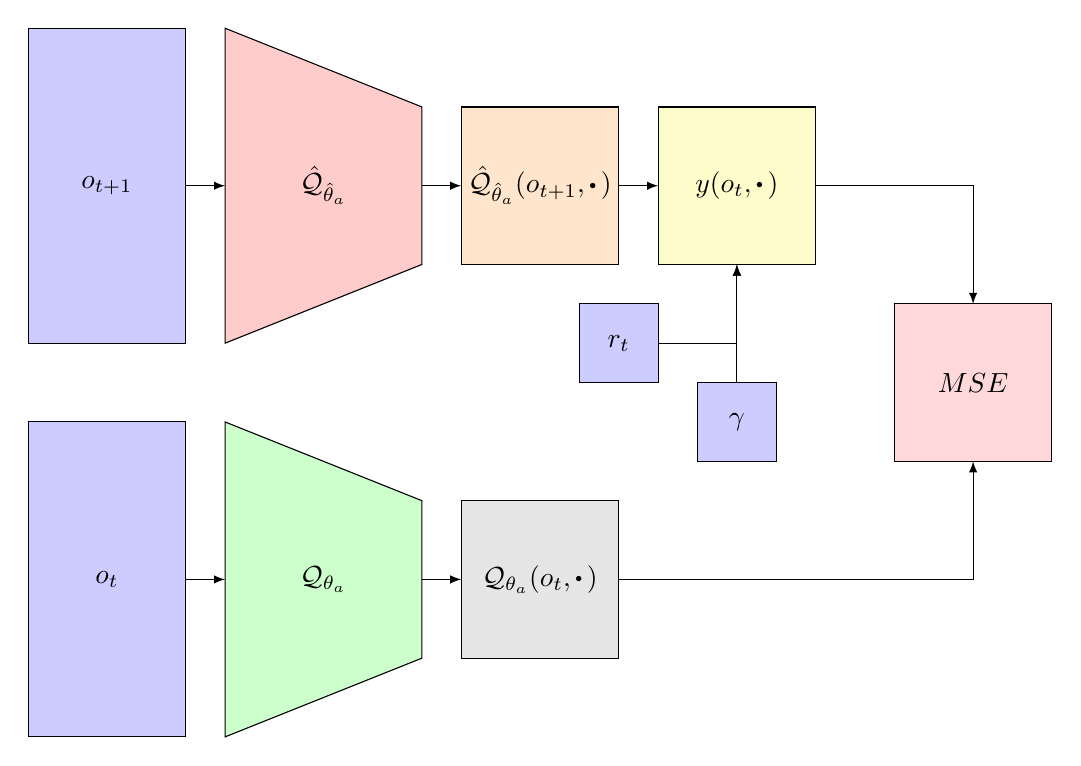
\begin{tikzpicture}[square/.style={regular polygon,regular polygon sides=4}, scale=1]
		% Q network
		\draw[fill=blue!20!white] (-1,-12) rectangle (1,-8);
	    \node at (0, -10) {$o_t$};

		\coordinate (A) at (1.5,-12);
		\coordinate (B) at (4,-11);
		\coordinate (C) at (4,-9);
		\coordinate (D) at (1.5,-8);
		\draw[fill=green!20!white] (A) -- coordinate[pos=.6] (AB) (B)--(C)
         --coordinate[pos=.45] (CD) (D)
         --coordinate[pos=.55] (DA) cycle;
	    \node at (2.75, -10) {$\mathcal{Q}_{\theta_a}$};

		\draw[fill=gray!20!white] (4.5,-11) rectangle (6.5,-9);
	    \node at (5.5, -10) {$\mathcal{Q}_{\theta_a}(o_t, \bigcdot\,)$};

	
		% target network
		\draw[fill=blue!20!white] (-1,-7) rectangle (1,-3);
	    \node at (0, -5) {$o_{t+1}$};

		\coordinate (A) at (1.5,-7);
		\coordinate (B) at (4,-6);
		\coordinate (C) at (4,-4);
		\coordinate (D) at (1.5,-3);
		\draw[fill=red!20!white] (A) -- coordinate[pos=.6] (AB) (B)--(C)
         --coordinate[pos=.45] (CD) (D)
         --coordinate[pos=.55] (DA) cycle;
	    \node at (2.75, -5) {$\hat{\mathcal{Q}}_{\hat{\theta}_a}$};

		\draw[fill=orange!20!white] (4.5,-6) rectangle (6.5,-4);
	    \node at (5.5, -5) {$\hat{\mathcal{Q}}_{\hat{\theta}_a}(o_{t+1}, \bigcdot\,)$};

		% cost function
		\draw[fill=blue!20!white] (6,-6.5) rectangle (7,-7.5);
	    \node at (6.5, -7) {$r_t$};

		\draw[fill=blue!20!white] (7.5,-7.5) rectangle (8.5,-8.5);
	    \node at (8, -8) {$\gamma$};

		\draw[fill=yellow!20!white] (7,-4) rectangle (9,-6);
	    \node at (8, -5) {$y(o_t,\bigcdot\,)$};

		\draw[fill=pink!60!white] (10,-6.5) rectangle (12,-8.5);
	    \node at (11, -7.5) {$MSE$};

		% arrows
		\draw[-latex] (4,-10) -- (4.5,-10);
		\draw[-latex] (1,-10) -- (1.5,-10);
		\draw[-latex] (4,-5) -- (4.5,-5);
		\draw[-latex] (1,-5) -- (1.5,-5);
		\draw[-latex] (6.5,-5) -- (7,-5);
		\draw[-latex] (7,-7) -- (8,-7) -- (8,-6);
		\draw[-latex] (9,-5) -- (11,-5) -- (11,-6.5);
		\draw[-latex] (6.5,-10) -- (11,-10) -- (11,-8.5);         
		\draw[-latex] (8,-7.5) -- (8,-6);
    \end{tikzpicture}

	\end{center}
  \caption{This figure illustrates the DQN agent. Briefly, the image $o_t$ is feed into the Q-network, and the image $o_{t+1}$ is feed into the target network. The Q-network outputs the Q-values for each action at time $t$, and the target network outputs the Q-values for each action at time $t+1$. Then, the reward, the discount factor, and Q-values of each action at time $t+1$ are used to compute the target values $y(o_t,\bigcdot\,)$. Finally, the goal is to minimise the MSE between the prediction of the Q-network and the target values.}
   \label{fig:DQN}
\end{figure}

\subsection{$DAI_{MC}$ agent \citep{DeepAIwithMCMC}}


\begin{figure}[h]
	\begin{center}
	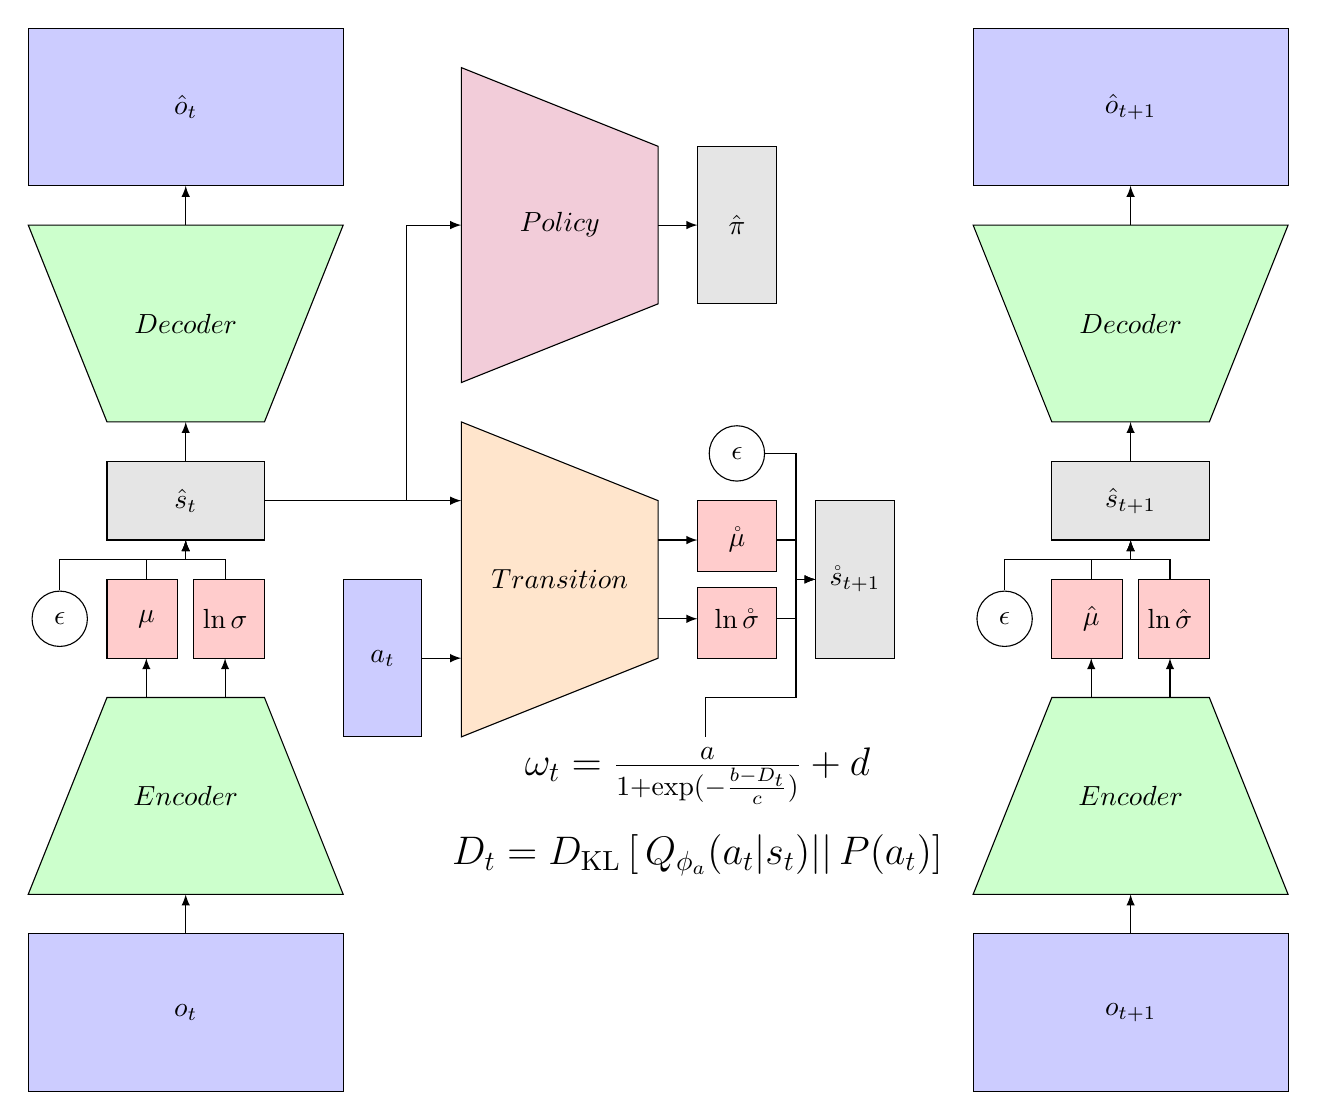
\begin{tikzpicture}[square/.style={regular polygon,regular polygon sides=4}]
		\coordinate (A) at (13.5,8);
		\coordinate (B) at (16,9);
		\coordinate (C) at (16,11);
		\coordinate (D) at (13.5,12);
		\draw[fill=purple!20!white] (A) -- coordinate[pos=.6] (AB) (B)--(C)
         --coordinate[pos=.45] (CD) (D)
         --coordinate[pos=.55] (DA) cycle;
	    \node at (14.75, 10) {$Policy$};

		\draw[-latex] (11,6.5) -- (12.8,6.5) -- (12.8,10) -- (13.5,10);
		\draw[-latex] (16, 10) -- (16.5, 10);
		
		\draw[fill=gray!20!white] (16.5,9) rectangle (17.5,11);
	    \node at (17, 10) {$\hat{\pi}$};


		\draw (16.6, 3.5) -- (16.6, 4) -- (17.75, 4) -- (17.75, 5.5);
	    \node at (16.5, 3) {\Large $\omega_t = \frac{a}{1 + \exp(-\frac{b - D_t}{c})} + d$};
		\node at (16.5, 2) {\Large $D_t = \kl{Q_{\phi_a}(a_t|s_t)}{P(a_t)}$};

		\pic{hmm};
    \end{tikzpicture}
	\end{center}
  \caption{This figure illustrates the $DAI_{MC}$ agent, which is composed of an encoder, a decoder, a transition network, and a policy network.}
  \label{fig:DAI_MC_agent}
\end{figure}


In this section, we review the $DAI_{MC}$ agent proposed by \citet{DeepAIwithMCMC}. The relevant code is available at the following URL: \url{https://github.com/zfountas/deep-active-inference-mc}. The $DAI_{MC}$ agent is composed of four deep neural networks illustrated in Figures \ref{fig:DAI_MC_agent} and \ref{fig:fountas_dnn}. The encoder $\mathcal{E}_{\phi_s}$ takes images as input, and outputs the mean and variance of the variational distribution over hidden state, i.e., $Q_{\phi_s}(s_t) = \mathcal{N}(s_t;\mu, \sigma)$, where $\mu, \sigma = \mathcal{E}_{\phi_s}(o_t)$. The decoder $\mathcal{D}_{\theta_o}$ takes a state as input, and outputs the parameters of a product of Bernoulli distributions, which can be interpreted as the expected (reconstructed) image $\hat{o}_t$, i.e., 
\begin{align*}
P(o_t|s_t) = \MultiBernoulli(o_t;\hat{o}_t),
\end{align*}
where $\hat{o}_t = \mathcal{D}_{\theta_o}(s_t)$ are the values predicted by the decoder, and $\MultiBernoulli(o_t;\hat{o}_t)$ is a product of Bernoulli distributions defined as:
$$\MultiBernoulli(o_t;\hat{o}_t) = \prod_{x,y} \text{Bernoulli}(o_t[x,y];\hat{o}_t[x,y]),$$
where $\text{Bernoulli}(\,\bigcdot\,;\,\bigcdot\,)$ is a Bernoulli distribution over the possible values of the pixel $o_t[x,y]$, parameterized by the parameter $\hat{o}_t[x,y]$. The transition network $\mathcal{T}_{\theta_s}$ takes a state-action pair as input, and outputs the mean and variance of a Gaussian distribution over hidden state, i.e., $P_{\theta_s}(s_{\tau+1}|s_\tau, a_\tau) = \mathcal{N}(s_{\tau+1};\mathring{\mu}, \frac{\mathring{\sigma}}{\omega_t})$, where $\mathring{\mu}, \mathring{\sigma} = \mathcal{T}_{\theta_s}(s_\tau, a_\tau)$, and $\omega_t$ is the top-down attention parameter modulating the precision of the transition mapping (see below). The policy network $\mathcal{P}_{\phi_a}$ takes a state as input, and outputs a distribution over actions, i.e., $Q_{\phi_a}(a_t|s_t) = \text{Cat}(a_t;\hat{\pi})$, where $\hat{\pi} = \mathcal{P}_{\phi_a}(s_t)$. Finally, the prior over actions is defined as follows:
\begin{align}
P(a_t) = \sum_{\pi \in \Pi} [\pi_t = a_t]P(\pi),\label{eq:initial_prior_actions}
\end{align}
where $\Pi$ is the set of all possible policies, $\pi_t$ is the action precribed by policy $\pi$ at time $t$, the bracket represents an indicator function that equals one if the condition within the bracket is satisfied and zero otherwise, and $P(\pi)$ is the prior over policies defined as: \begin{align*}
P(\pi) = \sigma[-G(\pi)],
\end{align*}
where $\sigma[\,\bigcdot\,]$ is the softmax function, and $G(\pi)$ is the expected free energy (EFE) of policy $\pi$, which is defined as:
\begin{align}
G(\pi) = \sum_{\tau = t}^T G_{\tau}(\pi) = \sum_{\tau = t}^T \mathbb{E}_{\tilde{Q}}\Big[ \ln Q(s_\tau, \theta|\pi) - \ln \tilde{P}(o_\tau, s_\tau,\theta|\pi) \Big],\label{eq:efe_fountas_defin}
\end{align}
where $\tilde{Q} = Q(o_\tau, s_\tau, \theta|\pi) = Q(\theta|\pi)Q(s_\tau|\theta,\pi)Q(o_\tau|s_\tau,\theta,\pi)$ and $\tilde{P}(o_\tau,s_\tau,\theta|\pi) = P(o_\tau|\pi)P(s_\tau|o_\tau,\pi)P(\theta|s_\tau,o_\tau,\pi)$. Up to now, we left the definition of the top-down attention parameter undefined. Formally, this parameter is computed as follows:
\begin{align*}
\omega_t = \frac{a}{1 + \exp(-\frac{b - D_t}{c})} + d,
\end{align*}
where $D_t = \kl{Q_{\phi_a}(a_t|s_t)}{P(a_t)}$, and $\{a, b, c, d\}$ are fixed hyperparameters. Intuitively, $\omega_t$ is high when the posterior over action is closed to the prior over action, and low when the posterior is far away from the prior. Finally, note that the prior over actions defined in \eqref{eq:initial_prior_actions} would requires the evaluation of an exponential number of policies. Because this is untractable in practice, \citet{DeepAIwithMCMC} implemented a Monte-Carlo tree search (MCTS) algorithm to evaluate the expected free energy of each action (see below). Finally, action selection is performed by sampling from the following distribution:
\begin{align*}
\tilde{P}(a_t) = \frac{N(\hat{s}_t, a_t)}{\sum_{\hat{a}_t}N(\hat{s}_t, \hat{a}_t)},
\end{align*}
where $\hat{s}_t$ is the current state of the environment, and $N(s_t, a_t)$ is the number of times actions $a_t$ has been visited from state $s_t$ during MCTS.

\begin{figure}[H]
	\begin{center}
	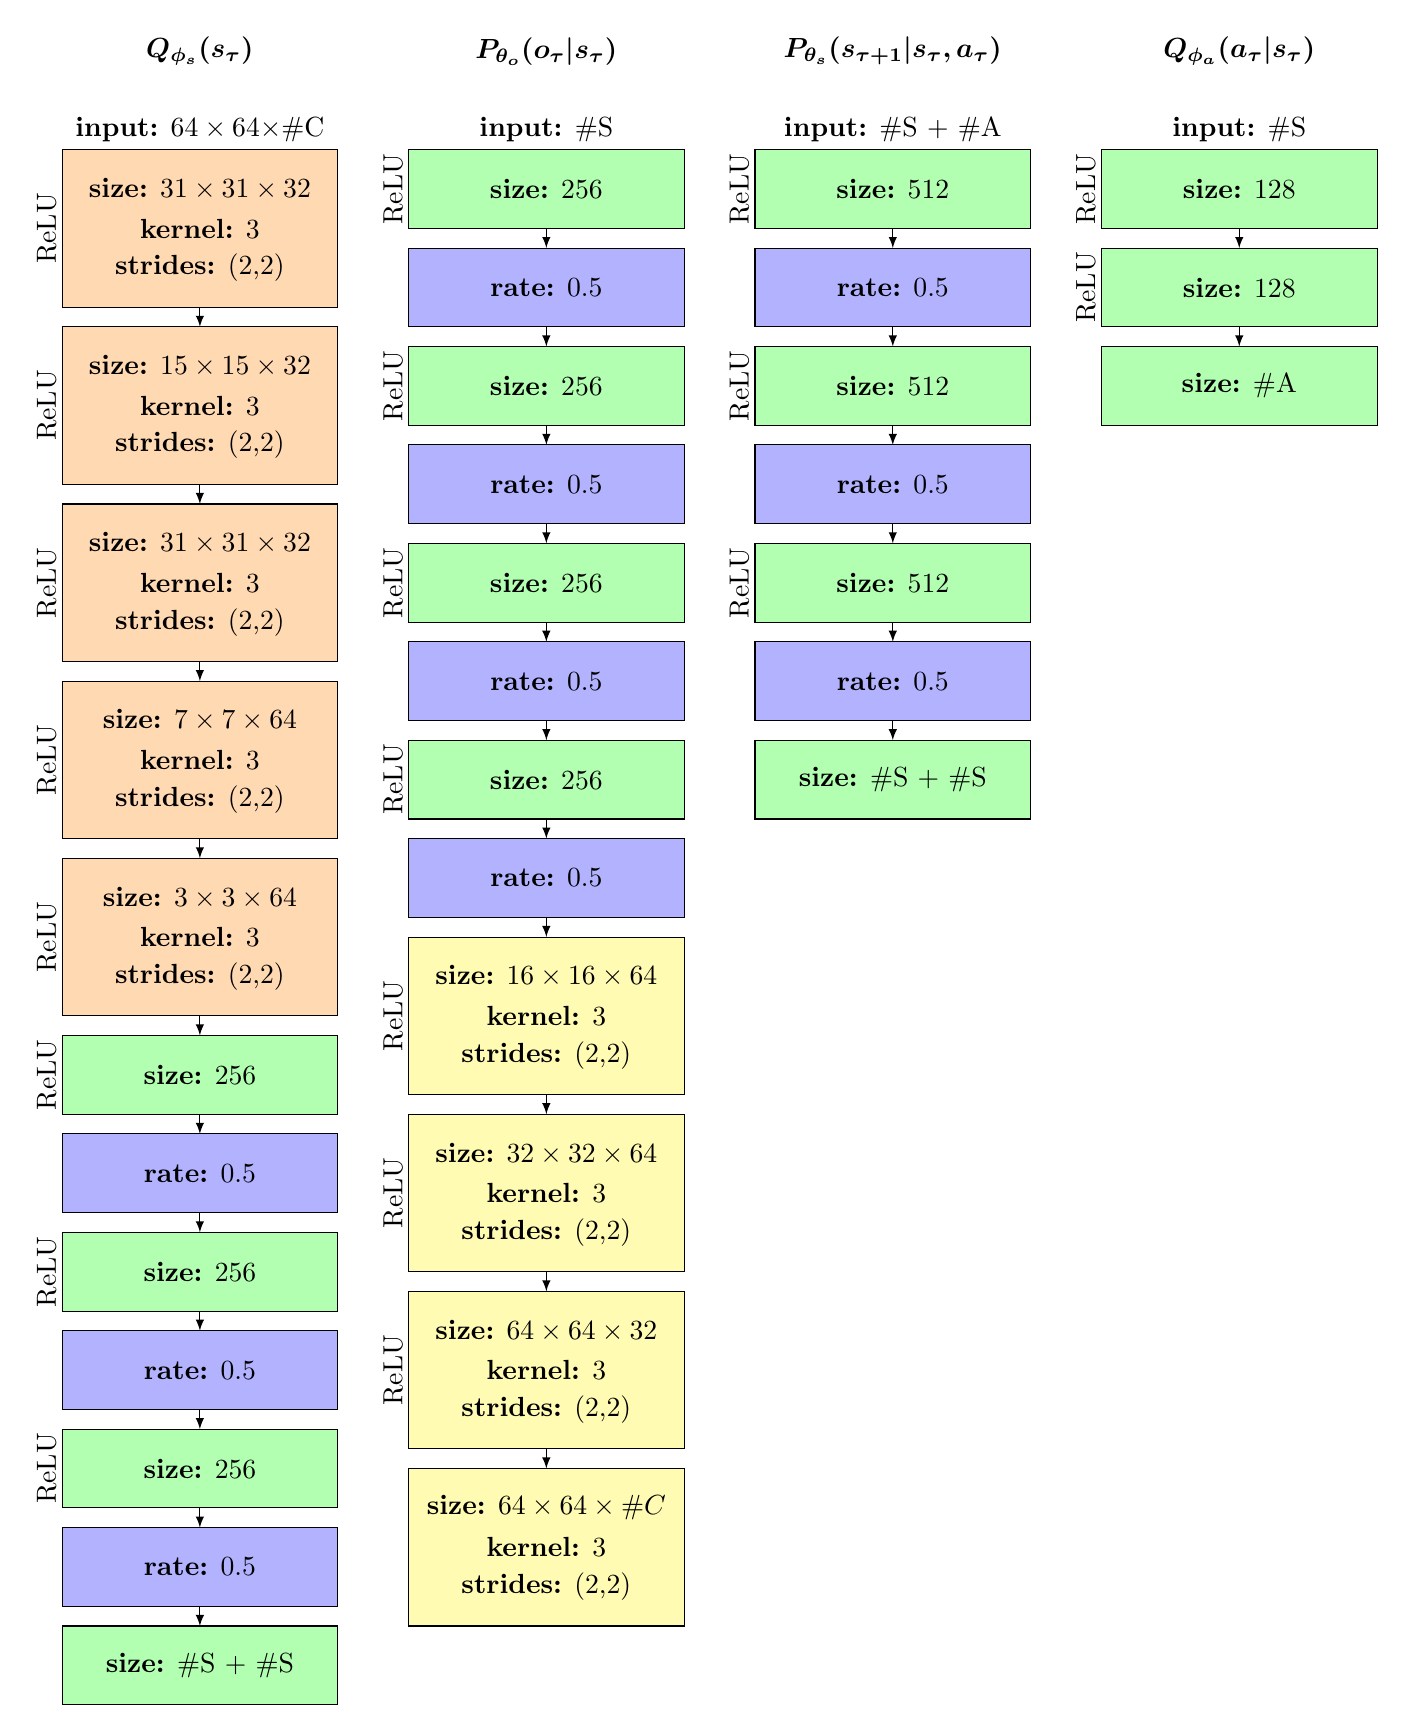
\begin{tikzpicture}
		%encoder
		\node (Q_s) at (-6.2,8) {$\bm{Q_{\phi_s}(s_\tau)}$};
		\node at (-6.2,7) {\textbf{input:} $64\times64\times$\#C};
		\pic{conv=-6.2/5.5/$31\times31\times32$/3/2/ReLU};
		\pic{conv=-6.2/3.25/$15\times15\times32$/3/2/ReLU};
		\pic{conv=-6.2/1/$31\times31\times32$/3/2/ReLU};
		\pic{conv=-6.2/-1.25/$7\times7\times64$/3/2/ReLU};
		\pic{conv=-6.2/-3.5/$3\times3\times64$/3/2/ReLU};
		\pic{dense=-6.2/-5.25/256/ReLU};
		\pic{dropout=-6.2/-6.5/0.5};
		\pic{dense=-6.2/-7.75/256/ReLU};
		\pic{dropout=-6.2/-9/0.5};
		\pic{dense=-6.2/-10.25/256/ReLU};
		\pic{dropout=-6.2/-11.5/0.5};
		\pic{dense=-6.2/-12.75/\#S + \#S/};

		\draw[-latex] (-6.2,4.75) -- (-6.2,4.5);
		\draw[-latex] (-6.2,2.5) -- (-6.2,2.25);
		\draw[-latex] (-6.2,0.25) -- (-6.2,0);
		\draw[-latex] (-6.2,-2) -- (-6.2,-2.25);
		\draw[-latex] (-6.2,-4.25) -- (-6.2,-4.5);
		\draw[-latex] (-6.2,-5.5) -- (-6.2,-5.75);
		\draw[-latex] (-6.2,-6.75) -- (-6.2,-7);
		\draw[-latex] (-6.2,-8) -- (-6.2,-8.25);
		\draw[-latex] (-6.2,-9.25) -- (-6.2,-9.5);
		\draw[-latex] (-6.2,-10.5) -- (-6.2,-10.75);
		\draw[-latex] (-6.2,-11.75) -- (-6.2,-12);

		%decoder
		\node (P_o) at (-1.8,8) {$\bm{P_{\theta_o}(o_\tau|s_\tau)}$};
		\node at (-1.8,7) {\textbf{input:} \#S};
		\pic{dense=-1.8/6/256/ReLU};
		\pic{dropout=-1.8/4.75/0.5};
		\pic{dense=-1.8/3.5/256/ReLU};
		\pic{dropout=-1.8/2.25/0.5};
		\pic{dense=-1.8/1/256/ReLU};
		\pic{dropout=-1.8/-0.25/0.5};
		\pic{dense=-1.8/-1.5/256/ReLU};
		\pic{dropout=-1.8/-2.75/0.5};
		\pic{upconv=-1.8/-4.5/$16\times16\times64$/3/2/ReLU};
		\pic{upconv=-1.8/-6.75/$32\times32\times64$/3/2/ReLU};
		\pic{upconv=-1.8/-9/$64\times64\times32$/3/2/ReLU};
		\pic{upconv=-1.8/-11.25/$64\times64\times\#C$/3/2/};

		\draw[-latex] (-1.8,5.75) -- (-1.8,5.5);
		\draw[-latex] (-1.8,4.5) -- (-1.8,4.25);
		\draw[-latex] (-1.8,3.25) -- (-1.8,3);
		\draw[-latex] (-1.8,2) -- (-1.8,1.75);
		\draw[-latex] (-1.8,0.75) -- (-1.8,0.5);
		\draw[-latex] (-1.8,-0.5) -- (-1.8,-0.75);
		\draw[-latex] (-1.8,-1.75) -- (-1.8,-2);
		\draw[-latex] (-1.8,-3) -- (-1.8,-3.25);
		\draw[-latex] (-1.8,-5.25) -- (-1.8,-5.5);
		\draw[-latex] (-1.8,-7.5) -- (-1.8,-7.75);
		\draw[-latex] (-1.8,-9.75) -- (-1.8,-10);

		% transition
		\node (P_s) at (2.6,8) {$\bm{P_{\theta_s}(s_{\tau+1}|s_\tau,a_\tau)}$};
		\node at (2.6,7) {\textbf{input:} \#S + \#A};
		\pic{dense=2.6/6/512/ReLU};
		\pic{dropout=2.6/4.75/0.5};
		\pic{dense=2.6/3.5/512/ReLU};
		\pic{dropout=2.6/2.25/0.5};
		\pic{dense=2.6/1/512/ReLU};
		\pic{dropout=2.6/-0.25/0.5};
		\pic{dense=2.6/-1.5/\#S + \#S/};

		\draw[-latex] (2.6,5.75) -- (2.6,5.5);
		\draw[-latex] (2.6,4.5) -- (2.6,4.25);
		\draw[-latex] (2.6,3.25) -- (2.6,3);
		\draw[-latex] (2.6,2) -- (2.6,1.75);
		\draw[-latex] (2.6,0.75) -- (2.6,0.5);
		\draw[-latex] (2.6,-0.5) -- (2.6,-0.75);
		
		% policy
		\node (Q_a) at (7,8) {$\bm{Q_{\phi_a}(a_\tau|s_\tau)}$};
		\node at (7,7) {\textbf{input:} \#S};
		\pic{dense=7/6/128/ReLU};
		\pic{dense=7/4.75/128/ReLU};
		\pic{dense=7/3.5/\#A/};

		\draw[-latex] (7,5.75) -- (7,5.5);
		\draw[-latex] (7,4.5) -- (7,4.25);

	\end{tikzpicture}
	\end{center}
	\caption{Neural networks architecture of the $DAI_{MC}$ agent. Orange blocks correspond to convolutional layers, green blocks correspond to fully connected layers, blue blocks correspond to dropout, and yellow blocks correspond to up-convolutional layers. For the dSprites environment, there are four actions (i.e., \#A = 4), ten states (i.e., \#S = 10), and only one channel (i.e., \#C = 1). For the Animal-AI environment, there are three actions (i.e., \#A = 3), ten states (i.e., \#S = 10), and three channels (i.e., \#C = 3).}
	\label{fig:fountas_dnn}
\end{figure}

\subsubsection{The Monte-Carlo tree search}

In this section, we describe the planning algorithm used by $DAI_{MC}$. At the beginning of an action-perception cycle, the agent is provided with an image $o_t$. This image can be feed into the encoder to get the mean vector $\mu$ of the posterior over the latent states, i.e., $Q_{\phi_s}(s_t) = \mathcal{N}(s_t;\mu, \sigma)$. Since $\mu$ is the mean of the Gaussian posterior, it can be interpreted as the maximum a posteriori (MAP) estimates of the latent states at time step $t$. This MAP estimate will constitute the root node of the Monte-Carlo tree search (MCTS).

The first step of the MCTS is to use the UCT criterion to determine which node in the tree should be expanded. Let the tree's root $\hat{s}_t$ be called the current node that is denoted $\hat{s}_\tau$. If the current node has no children, then it is selected for expansion. Alternatively, the child with the highest UCT criterion becomes the new current node and the process is iterated until we reach a leaf node (i.e. a node from which no action has previously been selected). The UCT criterion \citep{MCTS} of the child of $\hat{s}_\tau$ corresponding to action $\hat{a}_\tau$ is given by:
\begin{align*}
UCT(\hat{s}_\tau,\hat{a}_\tau) = - \bar{G}(\hat{s}_\tau,\hat{a}_\tau) + C_{explore} \cdot \frac{Q_{\phi_a}(a_\tau=\hat{a}_\tau|s_\tau=\hat{s}_\tau)}{1 + N(\hat{s}_\tau,\hat{a}_\tau)},
\end{align*}
where $\bar{G}(\hat{s}_\tau,\hat{a}_\tau)$ is the average expected free energy of taking action $\hat{a}_\tau$ in state $\hat{s}_\tau$, $C_{explore}$ is the exploration constant that modulates the amount of exploration at the tree level, $N(\hat{s}_\tau,\hat{a}_\tau)$ is the number of times action $\hat{a}_\tau$ was visited in state $\hat{s}_\tau$, and $Q_{\phi_a}(a_\tau=\hat{a}_\tau|s_\tau=\hat{s}_\tau)$ is the posterior probability of action $\hat{a}_\tau$ in state $\hat{s}_\tau$. 

Let $\mathring{s}_\tau$ be the (leaf) node selected by the above selection procedure. The MCTS then expands one of the children of $\mathring{s}_\tau$. The expansion uses the transition network to compute the mean $\mathring{\mu}$ of $P_{\theta_s}(s_{\tau+1}|s_\tau=\mathring{s}_\tau, a_\tau=\mathring{a}_\tau)$, which is viewed as a MAP estimate of the states at time $\tau+1$. Then, we need to estimate the cost of (virtually) taking action $\mathring{a}_\tau$. By definition, the cost is the expected free energy given by \eqref{eq:efe_fountas_defin}, and Monte-Carlo rollouts can be run to improve its estimation. The final step of the planning iteration is to back-propagate the cost of the newly expanded (virtual) action toward the root of the tree. Formally, we write the update as follows:
\begin{align}\label{eq:backprop}
\forall s \in \mathbb{A}_{\mathring{s}_\tau} \cup \{\mathring{s}_\tau \}, \quad \bm{G}_{s} \leftarrow \bm{G}_{s} + \bm{G}_{\mathring{s}_\tau},
\end{align}
where $\mathring{s}_\tau$ is node that was selected for expansion, and $\mathbb{A}_{\mathring{s}_\tau}$ is the set of all ancestors of $\mathring{s}_\tau$ in the tree. During the back propagation, we also update the number of visits as follows:
\begin{align}\label{eq:backprop_n}
\forall s \in \mathbb{A}_{\mathring{s}_\tau} \cup \{\mathring{s}_\tau \}, \quad \bm{N}_{s} \leftarrow \bm{N}_{s} + 1,
\end{align}
If we let $\bm{G}^{aggr}_s$ be the aggregated cost of an arbitrary node $s$ obtained by applying Equation \ref{eq:backprop} after each expansion, then we are now able to express $\bar{\bm{G}}_s$ formally as:
$$\bar{\bm{G}}_s = \frac{\bm{G}^{aggr}_s}{\bm{N}_s}.$$
Importantly, if the node $s$ corresponds to state reached from state $\hat{s}_\tau$ by performing action $\hat{a}_\tau$, then $G(\hat{s}_\tau, \hat{a}_\tau) = \bm{G}_s$ and $N(\hat{s}_\tau, \hat{a}_\tau) = \bm{N}_s$. The planning procedure described above ends when the maximum number of planning iterations is reached, or when a clear winner has been identified, i.e., if $\max_{a_t} P(a_t)-\frac{1}{\#A}>T_{dec}$ where $\#A$ is the number of possible actions, and $T_{dec}$ is a (threshold) hyperparameter.

\subsubsection{Derivation of the variational free energy}\label{ssec:derive_vfe_in_fountas}

Recall, the goal of the variational free energy is to make the approximate posterior $Q_\phi(s_t,a_t)$ as close as possible to the true posterior $P(s_t,a_t|o_{0:t})$, i.e.,
\begin{align*}
Q^*_\phi(s_t,a_t) = \argmin_{Q_\phi(s_t,a_t)} \kl{Q_\phi(s_t,a_t)}{P(s_t,a_t|o_{0:t})}.
\end{align*}
Using the d-separation criteria, it is straightforward to show that $s_t,a_t \indep o_{0:t-1} | s_{t-1},a_{t-1}$, and therefore:
\begin{align*}
Q^*_\phi(s_t,a_t) = \argmin_{Q_\phi(s_t,a_t)} \kl{Q_\phi(s_t,a_t)}{P(s_t,a_t|o_t,s_{t-1},a_{t-1})}.
\end{align*}
Using Bayes theorem, the linearity of expectation, and the fact that $Q_\phi(s_t,a_t)$ integrates to one:
\begin{align*}
Q_\phi^*(s_t,a_t) &= \argmin_{Q_\phi(s_t,a_t)} \kl{Q_\phi(s_t,a_t)}{P(s_t,a_t|o_t,s_{t-1},a_{t-1})}\\
&= \argmin_{Q_\phi(s_t,a_t)} \kl{Q_\phi(s_t,a_t)}{P(s_t,a_t,o_t,s_{t-1},a_{t-1})} + \underbrace{\ln P(o_t,s_{t-1},a_{t-1})}_{\text{Constant w.r.t }Q_\phi(s_t,a_t)}\\
&= \argmin_{Q_\phi(s_t,a_t)} \kl{Q_\phi(s_t,a_t)}{P(s_t,a_t,o_t,s_{t-1},a_{t-1})}.
\end{align*}
Using the d-separation criteria, it is straightforward to show that:
$$P(s_t,a_t,o_t,s_{t-1},a_{t-1}) = P_{\theta_o}(o_t|s_t)P(a_t)P_{\theta_s}(s_t|s_{t-1},a_{t-1})Q_{\phi}(s_{t-1}, a_{t-1}),$$
where $Q_\phi(s_{t-1}, a_{t-1})$ is the variational posterior obtained through the inference process at the previous time step. In the above equation, $Q_\phi(s_{t-1}, a_{t-1})$ was used to replace $P(s_{t-1}, a_{t-1})$, i.e., $Q_\phi(s_{t-1}, a_{t-1})$ was used as an empirical prior. Additionally, since $Q_\phi(s_{t-1}, a_{t-1})$ is a constant w.r.t $Q_\phi(s_t,a_t)$, the above minimization problem reduces to:
\begin{align}
Q^*_{\phi}(s_t,a_t)\quad &= \,\, \argmin_{\quad Q_{\phi}(s_t,a_t) \,\,\,\,\,\, \quad }\underbrace{\kl{Q_{\phi}(s_t,a_t)}{P_{\theta_o}(o_t|s_t)P(a_t)P_{\theta_s}(s_t|s_{t-1},a_{t-1})}}_{\text{variational free energy}}\label{eq:def_vfe_fountas}\\
&= \argmin_{Q_{\phi_a}(a_t|s_t)Q_{\phi_s}(s_t)}\, \mathbb{E}_{Q_{\phi_s}(s_t)}\Big[ \kl{Q_{\phi_a}(a_t|s_t)}{P(a_t)} \Big] + \kl{Q_{\phi_s}(s_t)}{P_{\theta_s}(s_t|s_{t-1},a_{t-1})}\nonumber\\
&\hspace{8.9cm}- \mathbb{E}_{Q_{\phi_s}(s_t)}\Big[\ln P_{\theta_o}(o_t|s_t)\Big].\nonumber
\end{align}
By comparing \eqref{eq:def_vfe_fountas} and \eqref{eq:efe_fountas_defin}, one can see an inconsistency. Namely, the parameter $\theta$ are seen as latent variables in the EFE definition but they are regarded as parameters in the VFE. This asks the question of whether the EFE is really the expectation of the VFE. To sum up, the $DAI_{MC}$ agent is equipped with four deep neural networks modelling $Q_{\phi_a}(a_t|s_t)$, $Q_{\phi_s}(s_t)$, $P_{\theta_s}(s_t|s_{t-1},a_{t-1})$, and $P_{\theta_o}(o_t|s_t)$. The weights of those networks are optimised using back-propagation to minimise the VFE given by \eqref{eq:def_vfe_fountas}. Note, \eqref{eq:def_vfe_fountas} decomposes into two KL-divergence terms that can be computed analytically, and the expectations can be approximated using a Monte-Carlo estimate. Also, because $P_{\theta_o}(o_t|s_t)$ is modelled as a product of Bernoulli distributions the logarithm of $P_{\theta_o}(o_t|s_t)$ reduces to the binary cross entropy.

\subsubsection{Independence assumptions and the expected freee energy}

The EFE as stated in \eqref{eq:efe_fountas_defin} needs to be re-arranged because it cannot be easily evaluated. First, using the product rule of probability one can see that $\tilde{Q} = Q(s_\tau, \theta|\pi) = Q(\theta|s_\tau,\pi)Q(s_\tau|\pi)$ and $\tilde{P}(o_\tau,s_\tau,\theta|\pi) = P(o_\tau|\pi)P(s_\tau|o_\tau,\pi)P(\theta|s_\tau,o_\tau,\pi)$. Using those two factorisations, the EFE given in \eqref{eq:efe_fountas_defin}, i.e.,
\begin{align*}
G_{\tau}(\pi) = \mathbb{E}_{\tilde{Q}}\Big[ \ln Q(s_\tau, \theta|\pi) - \ln \tilde{P}(o_\tau, s_\tau,\theta|\pi) \Big],
\end{align*}
can be re-arranged as follows:
\begin{align}
G_{\tau}(\pi) = &- \mathbb{E}_{\tilde{Q}}\Big[ \ln \tilde{P}(o_\tau|\pi)\Big]\nonumber\\
&+ \mathbb{E}_{\tilde{Q}}\Big[ \ln Q(s_\tau|\pi) - \ln \tilde{P}(s_\tau|o_\tau, \pi) \Big]\nonumber\\
&+ \mathbb{E}_{\tilde{Q}}\Big[ \ln Q(\theta|s_\tau, \pi) - \ln \tilde{P}(\theta|s_\tau,o_\tau,\pi) \Big].\label{eq:efe_rearrangedd}
\end{align}
\subsubsubsection{Re-arranging the second term of Equation \eqref{eq:efe_rearrangedd} according to \citet{DeepAIwithMCMC}}
In the supplementary material of \citep{DeepAIwithMCMC}, the second term of Equation \eqref{eq:efe_rearrangedd} is re-aranged as follows:
\begin{align}
\mathbb{E}_{\tilde{Q}}\Big[ \ln Q(s_\tau|\pi) - \ln \tilde{P}(s_\tau|o_\tau, \pi) \Big] &\delequal \mathbb{E}_{\tilde{Q}}\Big[ \ln Q(s_\tau|\pi) - \ln Q(s_\tau|o_\tau, \pi) \Big]\label{eq:switching_point}\\
&= \mathbb{E}_{Q(\theta|\pi)Q(s_\tau|\theta,\pi)Q(o_\tau|s_\tau,\theta,\pi)}\Big[ \ln Q(s_\tau|\pi) - \ln Q(s_\tau|o_\tau, \pi) \Big]\nonumber\\
&= \mathbb{E}_{Q(\theta|\pi)}\Big[ \mathbb{E}_{Q(s_\tau|\theta,\pi)}[\ln Q(s_\tau|\pi)] - \mathbb{E}_{Q(s_\tau|\theta,\pi)Q(o_\tau|s_\tau,\theta,\pi)}[\ln Q(s_\tau|o_\tau, \pi)] \Big]\nonumber\\
&= \mathbb{E}_{Q(\theta|\pi)}\Big[ \mathbb{E}_{Q(s_\tau|\theta,\pi)}[\ln Q(s_\tau|\pi)] - \mathbb{E}_{Q(o_\tau|\theta,\pi)Q(s_\tau,|o_\tau,\theta,\pi)}[\ln Q(s_\tau|o_\tau, \pi)] \Big],\nonumber
\end{align}
where in the first line a distribution was renamed, i.e., $\tilde{P}(s_\tau|o_\tau, \pi) \delequal Q(s_\tau|o_\tau, \pi)$. The next step in the derivation (c.f. supplementart material of \citet{DeepAIwithMCMC}) states the following:
\begin{align*}
\mathbb{E}_{\tilde{Q}}\Big[ \ln Q(s_\tau|\pi) - \ln Q(s_\tau|o_\tau, \pi) \Big] &= \mathbb{E}_{Q(\theta|\pi)}\Big[ \mathbb{E}_{Q(o_\tau|\theta,\pi)}[H[Q(s_\tau|o_\tau, \pi)]] - H[Q(s_\tau|\pi)] \Big].
\end{align*}
However, the above equation assumes that $s_\tau \indep \theta\,\, | \,\,\pi$ and $s_\tau \indep \theta \,\,| \,\,\pi, o_\tau$. In other words, the conditioning on $\theta$ has been dropped, i.e.,
\begin{align*}
\mathbb{E}_{Q(\theta|\pi)}\Big[ &\mathbb{E}_{Q(s_\tau|\theta,\pi)}[\ln Q(s_\tau|\pi)] - \mathbb{E}_{Q(o_\tau|\theta,\pi)Q(s_\tau,|o_\tau,\theta,\pi)}[\ln Q(s_\tau|o_\tau, \pi)] \Big] \\
&\neq \mathbb{E}_{Q(\theta|\pi)}\Big[ \mathbb{E}_{Q(s_\tau|\pi)}[\ln Q(s_\tau|\pi)] - \mathbb{E}_{Q(o_\tau|\theta,\pi)Q(s_\tau,|o_\tau,\pi)}[\ln Q(s_\tau|o_\tau, \pi)] \Big] \\
&= \mathbb{E}_{Q(\theta|\pi)}\Big[ \mathbb{E}_{Q(o_\tau|\theta,\pi)}\big[H[Q(s_\tau|o_\tau, \pi)]\big] - H[Q(s_\tau|\pi)] \Big].
\end{align*}
Whether this conditioning can be dropped or not depends on the factorisation of the distribution. In other words, those two assumptions (i.e., $s_\tau \indep \theta \,\,|\,\, \pi$ and $s_\tau \indep \theta \,\,| \,\,\pi, o_\tau$) would have to be checked using the d-separation criterion. Unfortunatly, as mentionned previously, the parameters $\theta$ are latent variables in \eqref{eq:efe_fountas_defin} but are regarded as parameters in \eqref{eq:def_vfe_fountas}, which makes the graphical model unclear. Instead of attempting to prove that $s_\tau \indep \theta \,\,|\,\, \pi$ and $s_\tau \indep \theta \,\,| \,\,\pi, o_\tau$, we propose an improvement of the derivation that do not make such independence assumptions.

\subsubsubsection{Improving the derivation of the second term of Equation  \eqref{eq:efe_rearrangedd}}

Restarting from the second term of Equation \eqref{eq:efe_rearrangedd}, we can  re-arange as follows:
\begin{align*}
\mathbb{E}_{\tilde{Q}}\Big[ \ln Q(s_\tau|\pi) - \ln \tilde{P}(s_\tau|o_\tau, \pi) \Big] &\delequal \mathbb{E}_{\tilde{Q}}\Big[ \ln Q(s_\tau|\pi) - \ln Q(s_\tau|o_\tau, \pi) \Big]\\
&= \mathbb{E}_{Q(s_\tau|\pi)Q(\theta,o_\tau|s_\tau,\pi)}\Big[ \ln Q(s_\tau|\pi)\Big] - \mathbb{E}_{Q(o_\tau|\pi)Q(s_\tau|o_\tau,\pi)Q(\theta|s_\tau,o_\tau,\pi)}\Big[ \ln Q(s_\tau|o_\tau, \pi) \Big]\\
&= \mathbb{E}_{Q(s_\tau|\pi)}\Big[ \ln Q(s_\tau|\pi)\Big] - \mathbb{E}_{Q(o_\tau|\pi)Q(s_\tau|o_\tau,\pi)}\Big[ \ln Q(s_\tau|o_\tau, \pi) \Big]\\
&= \mathbb{E}_{Q(o_\tau|\pi)}\Big[ H[Q(s_\tau|o_\tau, \pi)] \Big] - H[Q(s_\tau|\pi)],
\end{align*}
where in the first line a distribution was renamed, i.e., $\tilde{P}(s_\tau|o_\tau, \pi) \delequal Q(s_\tau|o_\tau, \pi)$, and the linearity of expectations was used between the second and third line. Importantly, the above derivation does not make any assumption of independence, and lead to a simpler result.

\subsubsubsection{Re-arranging the third term of Equation \eqref{eq:efe_rearrangedd} according to \citet{DeepAIwithMCMC}}

We now, focus on the third term of \eqref{eq:efe_rearrangedd}, which can be re-arranged as follows:
\begin{align*}
\mathbb{E}_{\tilde{Q}}\Big[ \ln Q(\theta|s_\tau, \pi) - \ln \tilde{P}(\theta|s_\tau,o_\tau,\pi) \Big] &\delequal \mathbb{E}_{\tilde{Q}}\Big[ \ln Q(\theta|s_\tau, \pi) - \ln Q(\theta|s_\tau,o_\tau,\pi) \Big] \\
&= \mathbb{E}_{\tilde{Q}}\Big[ \ln Q(o_\tau|s_\tau, \pi) - \ln Q(o_\tau|s_\tau,\theta,\pi) \Big],
\end{align*}
where $\tilde{P}(\theta|s_\tau,o_\tau,\pi)$ was renamed $Q(\theta|s_\tau,o_\tau,\pi)$, and Bayes theorem was used to get:
\begin{align*}
Q(\theta|s_\tau, \pi)
= \frac{Q(\theta|s_\tau,o_\tau,\pi)Q(o_\tau|s_\tau, \pi)}{Q(o_\tau|s_\tau,\theta,\pi)} \Leftrightarrow \frac{Q(\theta|s_\tau, \pi)}{Q(\theta|s_\tau,o_\tau,\pi)}
= \frac{Q(o_\tau|s_\tau, \pi)}{Q(o_\tau|s_\tau,\theta,\pi)}.
\end{align*}
Finally, by recalling that $\tilde{Q} = Q(o_\tau, s_\tau, \theta|\pi) = Q(\theta|\pi)Q(s_\tau|\theta,\pi)Q(o_\tau|s_\tau,\theta,\pi)$, and using the linearity of expectation, we get:
\begin{align*}
\mathbb{E}_{\tilde{Q}}\Big[ \ln Q(\theta|s_\tau, \pi) - \ln Q(\theta|s_\tau,o_\tau,\pi) \Big] &= \mathbb{E}_{Q(o_\tau,s_\tau|\pi)}\Big[ \ln Q(o_\tau|s_\tau, \pi)\Big] + \mathbb{E}_{Q(\theta|\pi)Q(s_\tau|\theta,\pi)}\Big[H[Q(o_\tau|s_\tau,\theta,\pi)] \Big]\\
&= \mathbb{E}_{Q(o_\tau|s_\tau,\pi)Q(s_\tau|\pi)}\Big[ \ln Q(o_\tau|s_\tau, \pi)\Big] + \mathbb{E}_{Q(\theta|\pi)Q(s_\tau|\theta,\pi)}\Big[H[Q(o_\tau|s_\tau,\theta,\pi)] \Big]\\
&= - \mathbb{E}_{Q(s_\tau|\pi)}\Big[ H\big[ Q(o_\tau|s_\tau, \pi) \big] \Big] + \mathbb{E}_{Q(\theta|\pi)Q(s_\tau|\theta,\pi)}\Big[H[Q(o_\tau|s_\tau,\theta,\pi)] \Big],
\end{align*}
where because $\ln Q(o_\tau|s_\tau, \pi)$ is a constant w.r.t $\theta$, we have been able to use:
\begin{align*}
\mathbb{E}_{Q(o_\tau,\theta,s_\tau|\pi)}[ \ln Q(o_\tau|s_\tau, \pi)] = \mathbb{E}_{Q(o_\tau,s_\tau|\pi)}[ \ln Q(o_\tau|s_\tau, \pi)].
\end{align*}

\subsubsubsection{The EFE according to \citet{DeepAIwithMCMC}}

If one follows the derivation proposed by \citet{DeepAIwithMCMC}, then the EFE is given by:
\begin{align}
G_{\tau}(\pi) = &- \mathbb{E}_{\tilde{Q}}\Big[ \ln \tilde{P}(o_\tau|\pi)\Big]\nonumber\\
&+ \mathbb{E}_{Q(\theta|\pi)}\Big[ \mathbb{E}_{Q(o_\tau|\theta,\pi)}\big[H[Q(s_\tau|o_\tau, \pi)]\big] - H[Q(s_\tau|\pi)] \Big]\nonumber\\
&+ \mathbb{E}_{Q(\theta|\pi)Q(s_\tau|\theta,\pi)}\Big[H[Q(o_\tau|s_\tau,\theta,\pi)] \Big] - \mathbb{E}_{Q(s_\tau|\pi)}\Big[ H\big[ Q(o_\tau|s_\tau, \pi) \big] \Big].\label{eq:efe_rearranged_fountas}
\end{align}
The way this expression is evaluated in practice will be described in Section \ref{ssec:discrepancies}.

\subsubsubsection{Our proposed improvement of the EFE}

If one follows our improved derivation, then the EFE is given by:
\begin{align*}
G_{\tau}(\pi) = &- \mathbb{E}_{\tilde{Q}}\Big[ \ln \tilde{P}(o_\tau|\pi)\Big]\\
&+ \mathbb{E}_{Q(o_\tau|\pi)}\Big[ H[Q(s_\tau|o_\tau, \pi)] \Big] - H[Q(s_\tau|\pi)],\\
&+ \mathbb{E}_{Q(\theta|\pi)Q(s_\tau|\theta,\pi)}\Big[H[Q(o_\tau|s_\tau,\theta,\pi)] \Big] - \mathbb{E}_{Q(s_\tau|\pi)}\Big[ H\big[ Q(o_\tau|s_\tau, \pi) \big] \Big].
\end{align*}

\subsubsection{Discrepancies between the paper and the code} \label{ssec:discrepancies}

In this section, we analyse the authors' implementation of $DAI_{MC}$ available on GitHub: \url{https://github.com/zfountas/deep-active-inference-mc/}. First, according to a private communication with one of the author, the code available on GitHub (on the 6th of June 2022) is not the same as the one used to run the experiements of the paper. Below, we describe the discrepancies between the paper and the code. For example, the computation of $\omega_t$ in the paper goes as follows:
\begin{align*}
\omega_t = \frac{a}{1 + \exp(-\frac{b - D_t}{c})} + d,
\end{align*}
while the code uses the following formula:
\begin{align*}
\omega_t = a\times \Bigg(1 - \frac{1}{1 + \exp\big(-\frac{D_t - b}{c}\big)}\Bigg) + d.
\end{align*}
Also, the paper states that MCTS is perfomed to compute the prior over policies during training. However, in the code, MCTS is only used when testing the model, i.e., no MCTS when training the agent. Additionally, the paper states that actions are selected by sampling from:
\begin{align*}
\tilde{P}(a_t) = \frac{N(\hat{s}_t, a_t)}{\sum_{\hat{a}_t}N(\hat{s}_t, \hat{a}_t)}.
\end{align*}
However, the code selects an entire sequence of actions $\pi = (\mathring{a}_t, \mathring{a}_{t+1}, ..., \mathring{a}_{t+n})$ recursively from the root node in the tree. At each step in the recursion, the node with the highest number of visits $\mathring{a}_\tau$ is selected. Then, actions cancelling each others are removed from the sequence, e.g., if $a_\tau = LEFT$ and $a_{\tau+1} = RIGHT$ then both actions are removed from the sequence. This procedure produces a new sequence of actions $\pi'$ of equal or smaller length. Finally, the entire sequence of actions $\pi'$  is performed in the environment. This avoids the repeatition of the planning process for each action-perception cycle (saving computational time), however, this also requires domain knowledge (to remove actions that cancel each others out).

Additionally, in the paper experiements are run in both: the disentanglement sprites environment and the animal AI environment. However, the code does not allow the replication of the results on the animal AI environment, i.e., the code handling the animal AI environment has been removed. Moreover, the evaluation of the expected free energy is non trivial (see below) and the details are not discussed in the paper. Before to explain how the terms of the EFE are computed, we introduce a notation that allows us to express those computational steps concisely. For example, we note: 
$$o^r_t \overset{i}{\rightarrow} \text{Encoder} \overset{s}{\rightarrow} \text{Transition} \overset{m}{\rightarrow} \mathring{s}^r_{t+1},$$
meaning that $o^r_t$ is used as \textit{input} ($\overset{i}{\rightarrow}$) for the encoder, then a state is \textit{sampled} ($\overset{s}{\rightarrow}$) from the distribution predicted by the encoder and used as input for the transition network, finally, the \textit{mean} ($\overset{m}{\rightarrow}$) of the distribution predicted by the transition network is usd as a maximum a posterior estimate of $\mathring{s}^r_{t+1}$. Note, the transition network takes two inputs (i.e., a state and an action), when using our concise notation, we implicitly assumes that the actions prescribed by the policy\footnote{$\pi$ is the policy for which the expected free energy is being computed.} $\pi$ are provided as input to the transition network. Also, for each time step $\tau$, the reward $r_\tau$ collected by the agent is encoded in the pixels of the image $o_\tau$ as explained in Figure \ref{fig:encoding_rewards_in_image} leading a new image $o_\tau^r$. As illustrated on the right of Figure \ref{fig:computation_of_extrinsic_value}, the encoder/decoder networks are trained to predict the resulting images $o_\tau^r$. The computation of the first term in equation \eqref{eq:efe_rearranged_fountas} is illustrated on the left of Figure \ref{fig:computation_of_extrinsic_value}. Concisely, we have:
$$o_t^r \overset{i}{\rightarrow} \text{Encoder} \overset{s}{\rightarrow} \text{Transition} \overset{s}{\rightarrow} \text{Decoder} \overset{m}{\rightarrow} \mathring{o}_{t+1}^r.$$
Next, a matrix ($\mathring{r}_{t+1}$) encoding the maximum reward that the agent can gather is used as parameter of Bernoulli distrubtions to compute the logarithm of the probability (i.e., $\bm{L}$) of the three first rows of the reconstructed image $\mathring{o}_{t+1}^r$. Note, as explained in Figure \ref{fig:encoding_rewards_in_image}, the three first rows contain the predicted reward obtained at time $t+1$. Finally, the mean of $\bm{L}$ is then computed and is multiplied by ten to get $\mathbb{E}_{\tilde{Q}}[\ln \tilde{P}(o_\tau|\pi)]$. Similarly, the computation of $H[Q(s_\tau|\pi)]$ goes as follows:
$$o_t^r \overset{i}{\rightarrow} \text{Encoder} \overset{s}{\rightarrow} \text{Transition} \rightarrow \mathring{\mu}, \ln \mathring{\sigma},$$
where $Q(s_\tau|\pi)$ is equated with $\mathcal{N}(s_\tau;\mathring{\mu}, \mathring{\sigma})$, and an analytical solution is used to compute the entropy of $Q(s_\tau|\pi)$. Next, the computation of $H[Q(o_\tau|s_\tau, \pi)]$ goes as follows:
$$o_t^r \overset{i}{\rightarrow} \text{Encoder} \overset{s}{\rightarrow} \text{Transition} \overset{s}{\rightarrow} \text{Decoder} \overset{m}{\rightarrow} \mathring{o}^r_{t+1},$$
where observation $\mathring{o}^r_{t+1}$ is equated to the parameters of the Bernoulli distribution $Q(o_\tau|s_\tau, \pi)$, and an analytical solution is used to compute $H[Q(o_\tau|s_\tau, \pi)]$. Surprisingly, another observation $\mathring{o}^r_{t+1}$ sampled exactly as before is equated to the parameters of the Bernoulli distribution $Q(o_\tau|s_\tau,\theta,\pi)$, and the same analytical solution is used to compute $H[Q(o_\tau|s_\tau,\theta,\pi)]$. Finally, $H[Q(s_\tau|o_\tau, \pi)]$ is computed by feeding $\mathring{o}^r_{t+1}$ back into the encoder to get the mean and log-variance of the Gaussian distribution $Q(s_\tau|o_\tau, \pi)$, and the analytical solution for the entropy of a Gaussian is used to compute $H[Q(s_\tau|o_\tau, \pi)]$.

To sum, two samples of $\mathring{o}^r_{t+1}$ (sampled as described in Figure \ref{fig:encoding_rewards_in_image}) have been equated to the parameters of two diferent distributions, i.e., $Q(o_\tau|s_\tau,\theta,\pi)$, and $Q(o_\tau|s_\tau, \pi)$. Additionally, a third sample of $\mathring{o}^r_{t+1}$ (sampled in the same way) has also used as input to the distribution $\tilde{P}(o_\tau|\pi)$. Lastly, while \citet{DeepAIwithMCMC} defines the EFE as in \eqref{eq:efe_rearranged_fountas}. The code contains an error where a plus is turned into a minus leading to the following definition of the EFE:
\begin{align*}
G_{\tau}(\pi) = &- \mathbb{E}_{\tilde{Q}}\Big[ \ln \tilde{P}(o_\tau|\pi)\Big]\nonumber\\
&\,{\color{red}-} \,\, \mathbb{E}_{Q(\theta|\pi)}\Big[ \mathbb{E}_{Q(o_\tau|\theta,\pi)}\big[H[Q(s_\tau|o_\tau, \pi)]\big] - H[Q(s_\tau|\pi)] \Big]\nonumber\\
&+ \mathbb{E}_{Q(\theta|\pi)Q(s_\tau|\theta,\pi)}\Big[H[Q(o_\tau|s_\tau,\theta,\pi)] \Big] - \mathbb{E}_{Q(s_\tau|\pi)}\Big[ H\big[ Q(o_\tau|s_\tau, \pi) \big] \Big],
\end{align*}
where the red minus should be a plus. Put simply, the current implementation of $DAI_{MC}$ contains errors. Thus, researhers should avoid benchmarking their approach against the current implementation of the $DAI_{MC}$ agent.

\begin{figure}
	\begin{center}
	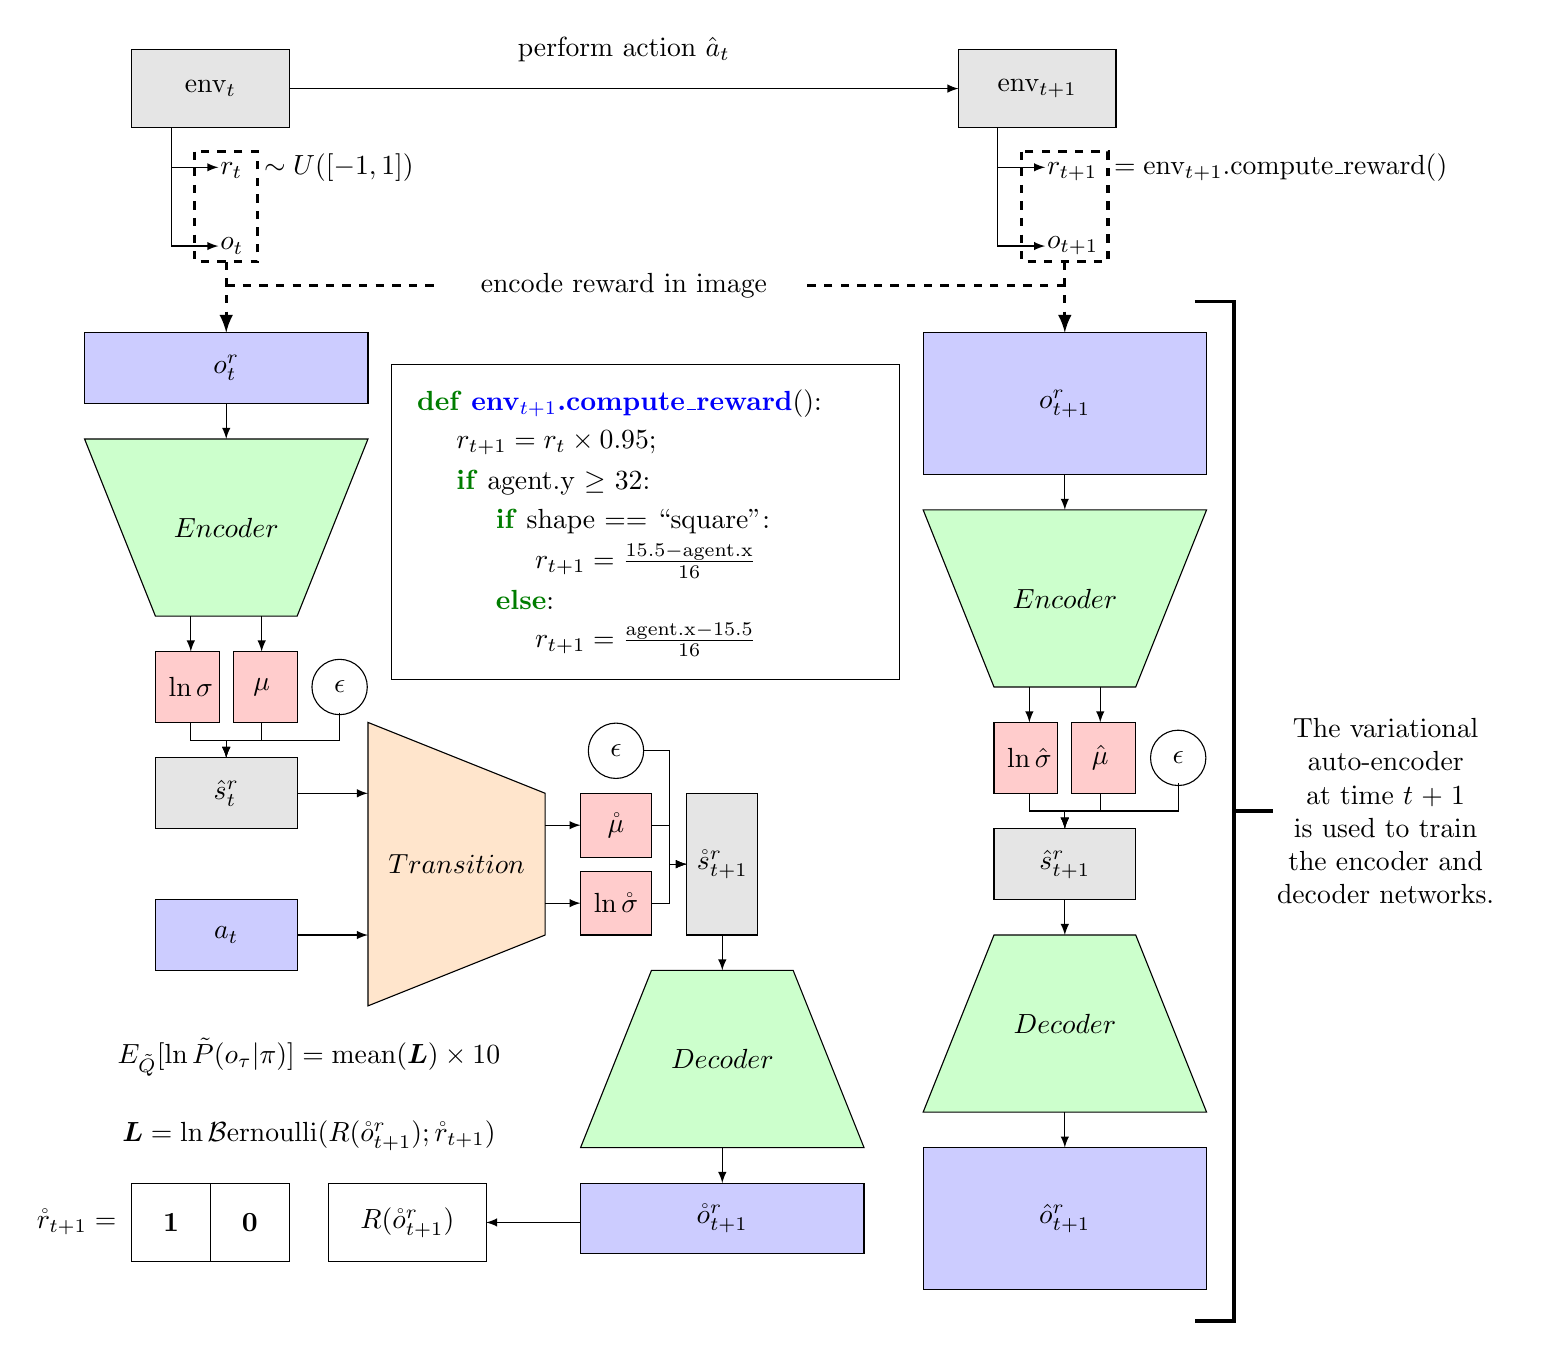
\begin{tikzpicture}[square/.style={regular polygon,regular polygon sides=4}]
		\draw[fill=gray!20!white] (-1,-0.5) rectangle (1,0.5);
		\node at (0, 0) {$\text{env}_t$};
		\draw[fill=gray!20!white] (9.5,-0.5) rectangle (11.5,0.5);
		\node at (10.5, 0) {$\text{env}_{t+1}$};
		\node at (5.25, 0.5) {$\text{perform action } \hat{a}_t$};
		\draw[-latex] (1,0) -- (9.5,0);
		\draw[-latex] (-0.5,-0.5) -- (-0.5,-1) -- (0.1,-1);
		\draw[-latex] (-0.5,-0.5) -- (-0.5,-2) -- (0.1,-2);

		\draw[-latex] (10,-0.5) -- (10,-1) -- (10.6,-1);
		\draw[-latex] (10,-0.5) -- (10,-2) -- (10.6,-2);

		\node[anchor=west] at (0, -1) {$r_t \,\,\, \sim U([-1, 1])$};
		\node[anchor=west] at (0, -2) {$o_t$};
		\draw[very thick, dashed] (-0.2,-0.8) rectangle (0.6,-2.2);
		\draw[very thick, dashed, -latex] (0.2,-2.2) -- (0.2,-3.1);

		\node[anchor=west] at (10.5, -1) {$r_{t+1} \,\, = \text{env}_{t+1}.\text{compute\_reward}()$};
		\node[anchor=west] at (10.5, -2) {$o_{t+1}$};
		\draw[very thick, dashed] (10.3,-0.8) rectangle (11.4,-2.2);
		\draw[very thick, dashed, -latex] (10.85,-2.2) -- (10.85,-3.1);

		\draw[very thick, dashed] (10.85,-2.5) -- (7.5,-2.5);
		\draw[very thick, dashed] (0.2,-2.5) -- (2.9,-2.5);
		\node at (5.25,-2.5) {encode reward in image};

		\pic[rotate=-90,xshift=4cm,yshift=19.85cm, scale=0.9]{vae=$o_{t+1}^r$/$\hat{\mu}$/$\ln \hat{\sigma}$/$\hat{s}_{t+1}^r$/$\hat{o}_{t+1}^r$};

		\draw[very thick] (12.5,-2.7) -- (13,-2.7) -- (13,-15.65) -- (12.5,-15.65);
		\draw[very thick] (13,-9.175) -- (13.5,-9.175);
		\node[anchor=west,text width=3cm,align=center] at (13.3,-9.175) {The variational auto-encoder at time $t+1$ is used to train the encoder and decoder networks.};
		
		\pic[rotate=-90, xshift=4cm,yshift=9.2cm, scale=0.9]{fountas=$o_t^r$/$\mu$/$\ln \sigma$/$\hat{s}_t^r$/$\mathring{o}_{t+1}^r$};

		\draw (1.5,-13.9) rectangle (3.5,-14.9);
		\draw (-1,-13.9) rectangle (1,-14.9);
		\draw (0,-13.9) -- (0,-14.9);
		\draw[-latex] (4.7,-14.4) -- (3.5,-14.4);
		\node at (-1.7,-14.4) {$\mathring{r}_{t+1} =$};
		\node at (0.5,-14.4) {$\bm{0}$};
		\node at (-0.5,-14.4) {$\bm{1}$};
		\node at (2.5,-14.4) {$R(\mathring{o}_{t+1}^r)$};

		\node at (1.25,-13.3) {$\bm{L} = \ln \mathcal{B}\text{ernoulli}(R(\mathring{o}_{t+1}^r); \mathring{r}_{t+1})$};
		\node at (1.25,-12.3) {$\mathbb{E}_{\tilde{Q}}[\ln \tilde{P}(o_\tau|\pi)] = \text{mean}(\bm{L}) \times 10$};

		\draw (2.3,-3.5) rectangle (8.75,-7.5);
		\node[anchor=west] at (2.5,-4) {{\color{GreenCode}\textbf{def}} {\color{BlueCode}\textbf{env$_{t+1}$.compute\_reward}}():};
		\node[anchor=west] at (3,-4.5) {$r_{t+1} = r_t \times 0.95;$};
		\node[anchor=west] at (3,-5) {{\color{GreenCode}\textbf{if}} agent.y $\geq$ 32:};
		\node[anchor=west] at (3.5,-5.5) {{\color{GreenCode}\textbf{if}} shape == ``square":};
		\node[anchor=west] at (4,-6) {$r_{t+1} = \frac{15.5 - \text{agent.x}}{16}$};
  		\node[anchor=west] at (3.5,-6.5) {{\color{GreenCode}\textbf{else}}:};
		\node[anchor=west] at (4,-7) {$r_{t+1} = \frac{\text{agent.x} - 15.5}{16}$};
    \end{tikzpicture}
	\end{center}
  \caption{This figure illustrates the the computation of $\mathbb{E}_{\tilde{Q}}[\ln \tilde{P}(o_\tau|\pi)]$. The environment at time $t$ provides the agent with an image $o_t$ and a reward $r_t$ randomly sampled from the interval $[-1;1]$. Then, action $\hat{a}_t$ is performed in the environment and the agent observes an image $o_{t+1}$ and a reward $r_{t+1}$, where $r_{t+1}$ is computed according to the function presented in the center of the image. Next, the reward at time $t$ and $t+1$ are encoded in the images at received at time $t$ and $t+1$, respectively, c.f., Figure \ref{fig:encoding_rewards_in_image} for details about the encoding. The encoded image at time $t+1$ (i.e., $o^r_{t+1}$) is then fed into the encoder, the re-parameterisation trick is then used to sample a state from the variational posterior. This states is fed into the decoder which tries to reconstruct the image inputed in the encoder. Once $\hat{o}^r_{t+1}$ has been computed, the weights of the encoder and decoder are learned using back-propagation. On the other hand, the encoded image at time $t$ (i.e., $o^r_t$) is used to compute the $\mathbb{E}_{\tilde{Q}}[\ln \tilde{P}(o_\tau|\pi)]$. More precisely, the $o^r_t$ is fed into the encoder, and a state is sampled from the variational posterior $Q_{\phi_s}(s_t)$. This state is then fed as input to the transition network along with the action prescribed by $\pi$ at time $t$, i.e., $a_t$. A state at time $t+1$ can then be sampled from the distribution predicted by the transition network. This state is then inputed into the decoder, which outputs $\mathring{o}^r_{t+1}$. Next, a matrix (i.e., $\mathring{r}_{t+1}$) encoding the maximum reward that the agent can gather is used as parameter of a Bernoulli distrubtions to compute the logarithm of the probability (i.e., $\bm{L}$) of the three first rows of $\hat{o}^r_{t+1}$, i.e., $R(\mathring{o}^r_{t+1})$. The mean of $\bm{L}$ is then computed and is multiplied by ten to get $\mathbb{E}_{\tilde{Q}}[\ln \tilde{P}(o_\tau|\pi)]$.}
   \label{fig:computation_of_extrinsic_value}
\end{figure}

\begin{figure}
	\begin{center}
	\begin{tikzpicture}[square/.style={regular polygon,regular polygon sides=4}]
	\node at (0,0) {\includegraphics[scale=2]{dSprites_reward_encoding}};
	\node[red] at (5.05,-1.45) {$-r_\tau$};
	\node[red] at (3.5,-1.45) {0};

	\node[red] at (-0.7,-1.45) {$r_\tau$};
	\node[red] at (0.75,-1.45) {0};

	\node[red] at (-5.05,-1.45) {$+$};
	\node[red] at (-3.55,-1.45) {$-$};
    \end{tikzpicture}
	\end{center}
  \caption{This figure illustrates how the reward $r_\tau \in [-1, 1]$ is encoded in image $o_\tau$. On the left, the plus and minus signs shows where the reward will be encoded in the image if the reward is positive or negative, respectively. In the middle, a positive reward is being encoded on the left side of the image. On the right, a negative reward is being encoded on the right of the image.}
   \label{fig:encoding_rewards_in_image}
\end{figure}

\subsection{$DAI_{VPG}$ agent \citep{DeepAI}}

In this section, we explain and discuss the approach of \citet{DeepAI}. The code is available at the following URL: \url{https://github.com/BerenMillidge/DeepActiveInference}. Note, even if the mathematics in the paper are based on the formalism of partially observable Markov decision process (POMDP), the code does not implement a encoder/decoder architecture, which means that the code implements a fully observable setting, i.e., MDP setting. Additionally, the $DAI_{VPG}$ is composed of three deep neural networks illustrated in Figures \ref{fig:beren_dnn} and \ref{fig:DAI_VPG_agent}. The first is the transition network that predicts the future observations based on the current observations and action, i.e., $\mathring{o}_{\tau+1} = \mathcal{T}_{\theta_o}(o_\tau, a_\tau)$. The second is the policy networks that models the variational distribution over actions $Q_{\phi_a}(a_\tau|o_\tau)$. The third is the critic network that predicts the expected free energy of each action given the current observation. Moreover, \citet{DeepAI} defines the prior over actions as follows:
\begin{align*}
P(a_\tau|o_\tau) = \sigma[-\zeta G(o_\tau, a_\tau)],
\end{align*}
where $\zeta$ is the precision of the prior over actions, $\sigma[\,\bigcdot\,]$ is a softmax function, and $G(o_\tau, a_\tau)$ is the expected free energy (EFE) of taking action $a_\tau$ when observing $o_\tau$. In the paper, the mathematics are based on the POMDP formalism. Therefore, $G(o_\tau, a_\tau)$ is denoted $G(s_\tau, a_\tau)$, and is defined as follows:
\begin{align}
G(s_\tau, a_\tau) = - r_\tau + \underbrace{\kl{Q(s_\tau)}{Q(s_\tau|o_\tau)}}_{\text{intrinsic value}} + \, \hat{\mathcal{G}}_{\hat{\theta}_a}(a_{\tau+1},s_{\tau+1}),\label{eq:efe_beren}
\end{align}
where $r_\tau$ is the reward gathered by the agent at time step $\tau$, and $\hat{\mathcal{G}}_{\hat{\theta}_a}(a_{\tau+1},s_{\tau+1})$ is the target network (i.e., a copy of the critic network whose weights are synchronised every $K$ iterations of learning). Now, remember that in the implementation, there is no encoder $Q(s_\tau)$ and no decoder $P(o_\tau|s_\tau)$. In other words, there are no hidden states $s_\tau$. With this in mind, it is unclear how the intrinsic value is computed. To answer this question, we read the code available on Github\footnote{We are referring to the version of the code that was available on the 6th of June 2022.} at the following URL: \url{https://github.com/BerenMillidge/DeepActiveInference}, in the file \url{active_inference_with_Tmodel.jl}. The answer to our question is at line 51 of the aforementioned file, and corresponds to the following equation:
\begin{align}
\text{intrinsic value} = \sum_{i} \Big[ o_{\tau+1}[i] - \mathring{o}_{\tau+1}[i] \Big]^2, \label{eq:intrisic_values}
\end{align}
where $o_{\tau+1}[i]$ is the i-th observation received at time step $\tau + 1$, and $\mathring{o}_{\tau+1}[i]$ is the value of the i-th observation (at time step $\tau + 1$) predicted by the transition network. More formally, the above formulation for the intrisic value correspond to the KL-divergence between two Gaussian distributions both having an identity covariance matrix, i.e.,
\begin{align*}
\text{intrinsic value} = \kl{Q(o_{\tau+1})}{P(o_{\tau+1}|o_\tau, a_\tau)} = \sum_{i} \Big[ o_{\tau+1}[i] - \mathring{o}_{\tau+1}[i] \Big]^2,
\end{align*}
where $P(o_{\tau+1}|o_\tau, a_\tau) = \mathcal{N}(o_{\tau+1};\mathring{o}_{\tau+1},I)$ and $Q(o_{\tau+1})$ is Gaussian distribution with mean vector $o_{\tau+1}$ and an identity covariance matrix. However, note that \eqref{eq:efe_beren} is the definition of the expected free energy in the POMDP setting. As explained by \citet{dacosta2020relationship}, the expected free energy in the MDP setting is given by:
\begin{align*}
G(a_{t:T-1},o_t) \approx \sum_{\tau+1}^T \kl{P(o_\tau |a_{\tau-1}, o_{\tau-1})}{P(o_\tau)},
\end{align*}
where $P(o_\tau)$ are the prior preferences of the agent (related to rewards in reinforcement learning), and $P(o_\tau |a_{\tau-1}, o_{\tau-1})$ is the transition mapping. Importantly, this definition for the expected free energy does not decomposes into an extrinsic and intrinsic term as in \eqref{eq:efe_beren}. Thus, (as it stands) the implementation of the $DAI_{VPG}$ agent is a mixture between the POMDP and MDP setting, where the generative model corresponds to a MDP, and the expected free energy is adapted from the POMDP setting.

We conclude this section by dicussing the training procedure of the transition, policy and critic networks. As explained in the paper, the transition network is trained to minimise the variational free enery. Additionally, because of the Gaussian assumptions mentionned above, the KL-divergence reduces to the mean square error (MSE). Thus, the transition network is updated to minimise the MSE between the observations made by the agent at time $\tau + 1$, and the observations ($\mathring{o}_{\tau+1}$) predicted by the transition network, i.e., 
\begin{align*}
\theta_o^* = \argmin_{\theta_o} \text{MSE}\Big[o_{\tau+1}, \mathring{o}_{\tau+1}\Big],
\end{align*}
where $\mathring{o}_{\tau+1} = \mathcal{T}_{\theta_o}(o_\tau, a_\tau)$. The policy network is trained to minimise the KL-divergence between the variational posterior over actions $Q_{\phi_a}(a_\tau|o_\tau)$ and the prior over actions $P(a_\tau|o_\tau)$, i.e., 
\begin{align*}
\phi_a^* = \argmin_{\phi_a} \kl{Q_{\phi_a}(a_\tau|o_\tau)}{P(a_\tau|o_\tau)},
\end{align*}
which minimises the variational free energy. Finally, the critic is trained by minimising the MSE between the target EFE as defined in \eqref{eq:efe_beren} and the ouput of the critic:
\begin{align*}
\theta_a^* = \argmin_{\theta_a} \text{MSE}\Big[G(o_\tau, \bigcdot\,), \mathcal{G}_{\theta_a}(o_\tau, \bigcdot\,)\Big].
\end{align*}

\begin{figure}[H]
	\begin{center}
	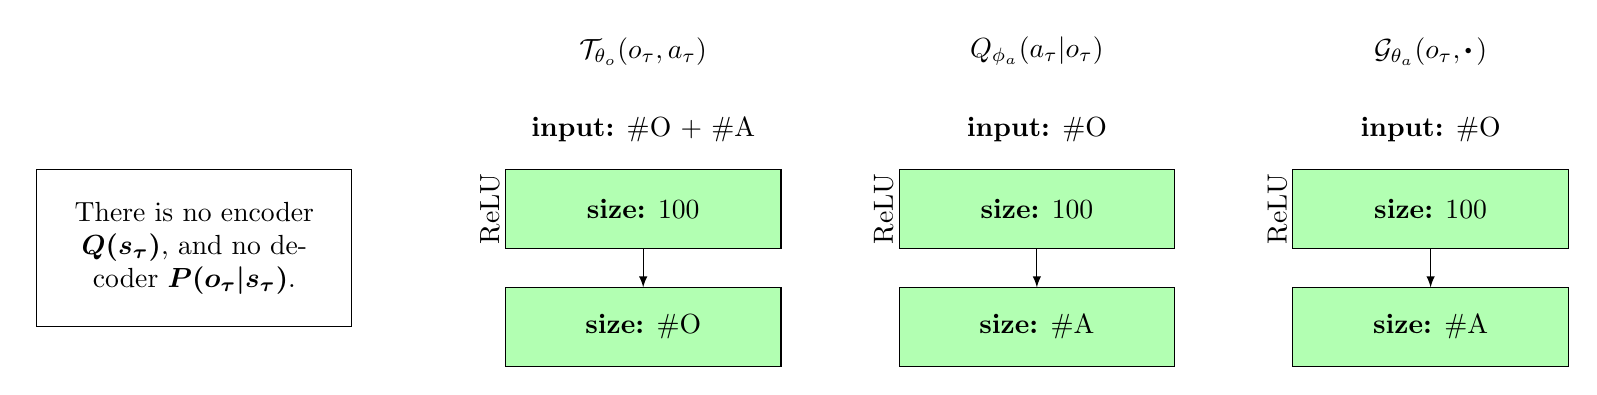
\begin{tikzpicture}
		% encoder and decoder
		\node[text width=4cm, align=center] at (-5.7,5.5) {There is no encoder $\bm{Q(s_\tau)}$, and no decoder $\bm{P(o_\tau|s_\tau)}$.};
		\draw (-7.7,4.5) rectangle (-3.7,6.5);
		
		% transition
		\node at (0,8) {$\mathcal{T}_{\theta_o}(o_\tau, a_\tau)$};
		\node at (0,7) {\textbf{input:} \#O + \#A};
		\pic{dense=0/5.75/100/ReLU};
		\pic{dense=0/4.25/\#O/};
		\draw[-latex] (0,5.5) -- (0,5);

		% policy
		\node at (5,8) {$Q_{\phi_a}(a_\tau| o_\tau)$};
		\node at (5,7) {\textbf{input:} \#O};
		\pic{dense=5/5.75/100/ReLU};
		\pic{dense=5/4.25/\#A/};
		\draw[-latex] (5,5.5) -- (5,5);

		% critic
		\node at (10,8) {$\mathcal{G}_{\theta_a}(o_\tau, \bigcdot\,)$};
		\node at (10,7) {\textbf{input:} \#O};
		\pic{dense=10/5.75/100/ReLU};
		\pic{dense=10/4.25/\#A/};
		\draw[-latex] (10,5.5) -- (10,5);
	\end{tikzpicture}
	\end{center}
	\caption{Neural networks architecture of the $DAI_{VPG}$ agent. Green blocks correspond to fully connected layers. The first neural network is the transition network that takes as input the observation and action at time step $\tau$, and outputs the mean of a Gaussian distribution over observation at time step $\tau + 1$. The second neural network is the policy network that models the variational posterior over actions. The third neural network is the critic that takes as input an observation and outputs the expected free energy of each action.}
	\label{fig:beren_dnn}
\end{figure}

\begin{figure}[H]
	\begin{center}
	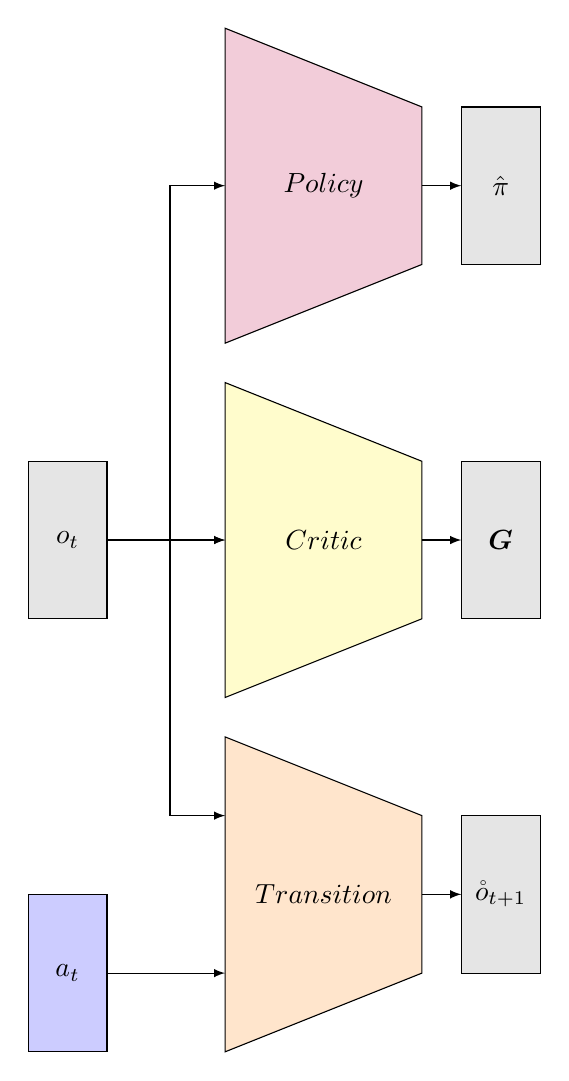
\begin{tikzpicture}[square/.style={regular polygon,regular polygon sides=4}]
		\coordinate (A) at (13.5,12.5);
		\coordinate (B) at (16,13.5);
		\coordinate (C) at (16,15.5);
		\coordinate (D) at (13.5,16.5);
		\draw[fill=purple!20!white] (A) -- coordinate[pos=.6] (AB) (B)--(C)
         --coordinate[pos=.45] (CD) (D)
         --coordinate[pos=.55] (DA) cycle;
	    \node at (14.75, 14.5) {$Policy$};
		\draw[-latex] (12.8,6.5) -- (12.8,14.5) -- (13.5,14.5);
		\draw[-latex] (16, 14.5) -- (16.5, 14.5);
		\draw[fill=gray!20!white] (16.5,13.5) rectangle (17.5,15.5);
	    \node at (17, 14.5) {$\hat{\pi}$};

		\coordinate (A) at (13.5,8);
		\coordinate (B) at (16,9);
		\coordinate (C) at (16,11);
		\coordinate (D) at (13.5,12);
		\draw[fill=yellow!20!white] (A) -- coordinate[pos=.6] (AB) (B)--(C)
         --coordinate[pos=.45] (CD) (D)
         --coordinate[pos=.55] (DA) cycle;
	    \node at (14.75, 10) {$Critic$};

		\draw[-latex] (12.8,6.5) -- (12.8,10) -- (13.5,10);
		\draw[-latex] (16, 10) -- (16.5, 10);
		
		\draw[fill=gray!20!white] (16.5,9) rectangle (17.5,11);
	    \node at (17, 10) {$\bm{G}$};

		\draw[fill=gray!20!white] (11,9) rectangle (12,11);
	    \node at (11.5, 10) {$o_t$};

		\draw[fill=blue!20!white] (11,3.5) rectangle (12,5.5);
	    \node at (11.5, 4.5) {$a_t$};

		\coordinate (A) at (13.5,3.5);
		\coordinate (B) at (16,4.5);
		\coordinate (C) at (16,6.5);
		\coordinate (D) at (13.5,7.5);
		\draw[fill=orange!20!white] (A) -- coordinate[pos=.6] (AB) (B)--(C)
         --coordinate[pos=.45] (CD) (D)
         --coordinate[pos=.55] (DA) cycle;
	    \node at (14.75, 5.5) {$Transition$};


		\draw[fill=gray!20!white] (16.5,4.5) rectangle (17.5,6.5);
	    \node at (17, 5.5) {$\mathring{o}_{t+1}$};

		\draw[-latex] (12,4.5) -- (13.5,4.5);
		\draw[-latex] (12,10) -- (13.5,10);
		\draw[-latex] (12.8,6.5) -- (13.5,6.5);

		\draw[-latex] (16,5.5) -- (16.5,5.5);

    \end{tikzpicture}
	\end{center}
  \caption{This figure illustrates the DAI agent. The only new part is the policy network, which takes as input the hidden state at time $t$ and ouputs the the parameters $\hat{\pi}$ of the variational posterior over actions. Importantly, the DAI takes actions based on the EFE.}
   \label{fig:DAI_VPG_agent}
\end{figure}

\subsection{$DAI_{RHI}$ agent \citep{rood2020deep}}

In this section, we quickly explain and discuss the approach of \citet{rood2020deep}. Put simply, this paper proposes a variational auto-encoder (VAE), which is able to account for experiemental results that were observed in the context of the rubber-hand illusion (RHI) experiement. The RHI is an experiement in which an agent (i.e., either a human or a computer) is able to move an arm in a 3D space. However, the agent does not observe the real position of the arm, instead, the agent sees an artificial hand placed in a different location. This can be implemented using virtual reality (for humans) or within a simulator (for computers). Since, \citet{rood2020deep} restricted themself to the context of a VAE, this approach can not be considered as a complete implementation of deep active inference. More precisely, the transition and critic (or policy) networks are missing.

\subsection{$DAI_{HR}$ agent \citep{sancaktar2020endtoend,DAI_HR,DAI_HR2}}

In this section, we quickly explain and discuss the following approaches: \citet{sancaktar2020endtoend}, \citet{DAI_HR}, and \citet{DAI_HR2}. Briefly, those papers propose a free energy minimisation scheme based on a single decoder network, which is used to control a Nao, TIAGo, and iCub robots, respectively. Since, \citet{sancaktar2020endtoend,DAI_HR,DAI_HR2} restricted themself to the context of a single decoder, this approach can not be considered as a complete implementation of deep active inference. More precisely, the encoder, transition and critic (or policy) networks are missing.

\subsection{$DAI_{FA}$ agent \citep{DAI_Kai}} \label{ssec:dai_approach}

In this section, we review the approach proposed by \citet{DAI_Kai}. The original code of this paper is available on GitHub at the following URL: \url{https://github.com/kaiu85/deepAI_paper}. Put simply, this approach is composed of four deep neural networks. The encoder $\mathcal{E}_{\phi_s}$ models the approximate posterior over states $Q_{\phi_s}(s_t|s_{t-1}, o_t)$ as a Gaussian distribution, i.e., $Q_{\phi_s}(s_t|s_{t-1}, o_t) = \mathcal{N}(s_t;\mu, \sigma)$ where $\mu, \sigma = \mathcal{E}_{\phi_s}(s_{t-1}, o_t)$. The decoder $\mathcal{D}_{\theta_o}$ models the likelihood mapping $P_{\theta_o}(o_\tau|s_\tau)$ as a Gaussian distribution, i.e., $P_{\theta_o}(o_\tau|s_\tau) = \mathcal{N}(o_\tau;\mu_o, \sigma_o)$ where $\mu_o, \sigma_o = \mathcal{D}_{\theta_o}(s_\tau)$. The transition network $\mathcal{T}_{\theta_s}$ models the transition mapping $P_{\theta_s}(s_\tau|s_{\tau-1})$ as a Gaussian distribution, i.e., $P_{\theta_s}(s_\tau|s_{\tau-1}) = \mathcal{N}(s_\tau;\mathring{\mu}, \mathring{\sigma})$ where $\mathring{\mu}, \mathring{\sigma} = \mathcal{T}_{\theta_s}(s_{\tau-1})$. Finally, the policy network $\mathcal{P}_{\theta_a}$ models the prior over actions $P_{\theta_a}(a_\tau|s_\tau)$ as a Gaussian distribution, i.e., $P_{\theta_a}(a_\tau|s_\tau) = \mathcal{N}(a_\tau;\mu_a, \sigma_a)$ where $\mu_a, \sigma_a = \mathcal{P}_{\theta_a}(s_\tau)$. Figure \ref{fig:kai_dnn} illustrates the architectures of those deep neural networks. Importantly, the experiments were run in the MountainCar environment, which means that the agent is observing the x position of the car $o_\tau^x$. Additionally, according to the idea of proprioception, the agent observes its own action, i.e., $o^a_{\tau-1} = a_{\tau-1}$ where $a_{\tau-1}$ is the action performed by the agent at time $\tau-1$. In what follows, we let $o_\tau = (o^x_\tau, o^a_{\tau-1})$ be the concatenation of the x position of the car and the action taken by the agent. Then, \citet{DAI_Kai} defines the free action objective as the cumulated variational free energy over time:
\begin{align*}
FA(o_{1:T}, \phi, \theta) = \sum_{\tau = 1}^T \Bigg[\underbrace{\overbrace{- \mathbb{E}_{Q_{\phi_s}(s_\tau|s_{\tau-1}, o_\tau)}\Big[\ln P_{\theta_o}(o_\tau|s_\tau)\Big]}^{\text{accuracy}} + \overbrace{\kl{Q_{\phi_s}(s_\tau|s_{\tau-1}, o_\tau)}{P_{\theta_s}(s_\tau|s_{\tau-1})}}^{\text{complexity}} }_{\text{VFE}_\tau}\Bigg],
\end{align*}
where $s_0 = (0, ..., 0)$ is a vector full of zeros representing the initial hidden state, $T$ is the time horizon, $P_{\theta_o}(o_\tau|s_\tau)$, $Q_{\phi_s}(s_\tau|s_{\tau-1}, o_t)$, $P_{\theta_s}(s_\tau|s_{\tau-1})$ are modeled using Gaussian distribution whose parameters are predicted by the decoder, encoder and transition network, respectively. Figure \ref{fig:kai_fa_estimate} illustrates the computation of the free action objective, and the action-perception cycle of the agent. The first action-perception cycle is initiated when the intital hidden state $s_0$ is being fed into the policy network, which outputs the parameters of a Gaussian distribution over action. Then, an action $a_0$ is sampled from this Gaussian, and executed in the environment leading to a new observation $o_1^x$. Next, the action $a_0$ is concatenate with $o_1^x$ to form $o_1$. The observation $o_1$ and the state $s_0$ are then fed into the encoder that outputs the parameters of a Gaussian distribution over $s_1$. Lastly, a state is sampled from this Gaussian distribution and is used as input to the next action-perception cycle. This process continues until reaching the time horizon.

\begin{figure}[H]
	\begin{center}
	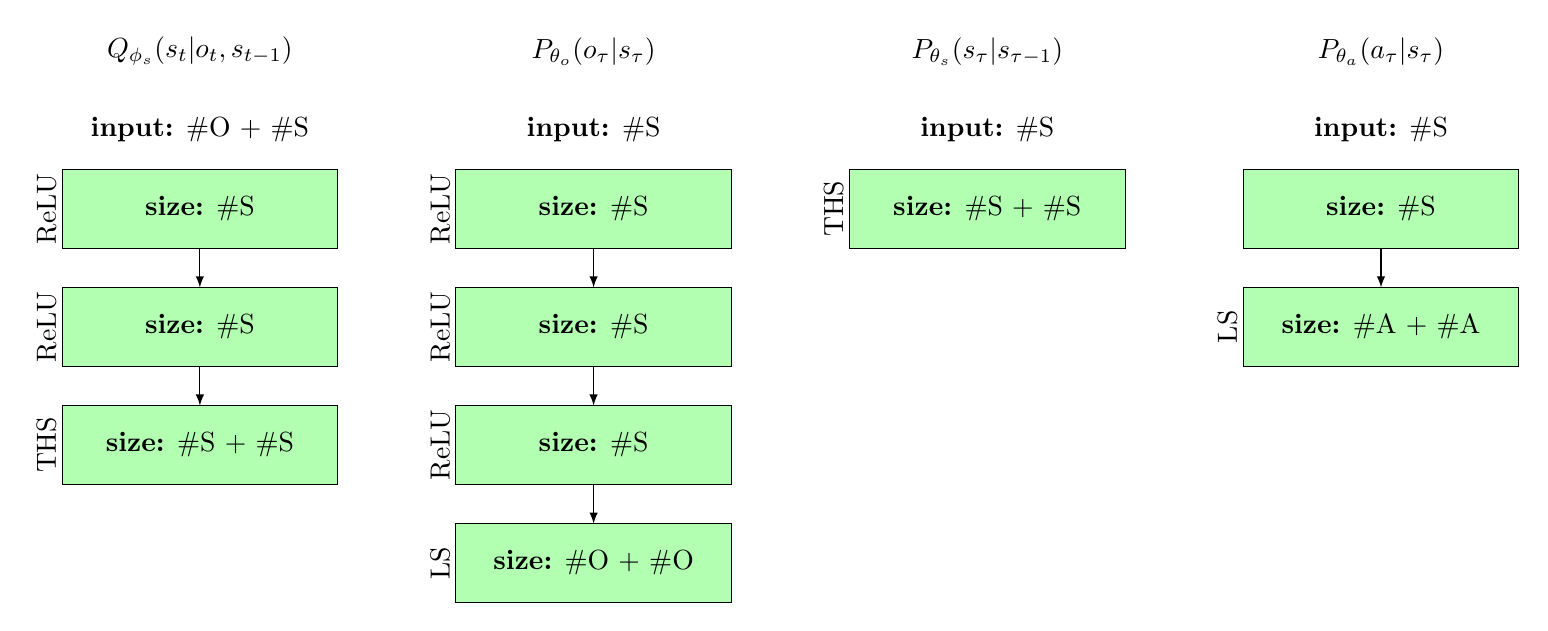
\begin{tikzpicture}
		% encoder
		\node at (-5,8) {$Q_{\phi_s}(s_t|o_t, s_{t-1})$};
		\node at (-5,7) {\textbf{input:} \#O + \#S};
		\pic{dense=-5/5.75/\#S/ReLU};
		\pic{dense=-5/4.25/\#S/ReLU};
		\pic{dense=-5/2.75/\#S + \#S/THS};
		\draw[-latex] (-5,5.5) -- (-5,5);
		\draw[-latex] (-5,4) -- (-5,3.5);

		% decoder
		\node at (0,8) {$P_{\theta_o}(o_\tau|s_\tau)$};
		\node at (0,7) {\textbf{input:} \#S};
		\pic{dense=0/5.75/\#S/ReLU};
		\pic{dense=0/4.25/\#S/ReLU};
		\pic{dense=0/2.75/\#S/ReLU};
		\pic{dense=0/1.25/\#O + \#O/LS};
		\draw[-latex] (0,5.5) -- (0,5);
		\draw[-latex] (0,4) -- (0,3.5);
		\draw[-latex] (0,2.5) -- (0,2);

		% transition
		\node at (5,8) {$P_{\theta_s}(s_\tau|s_{\tau-1})$};
		\node at (5,7) {\textbf{input:} \#S};
		\pic{dense=5/5.75/\#S + \#S/THS};

		% policy
		\node at (10,8) {$P_{\theta_a}(a_\tau| s_\tau)$};
		\node at (10,7) {\textbf{input:} \#S};
		\pic{dense=10/5.75/\#S/};
		\pic{dense=10/4.25/\#A + \#A/LS};
		\draw[-latex] (10,5.5) -- (10,5);
	\end{tikzpicture}
	\end{center}
	\caption{Neural networks architecture of the $DAI_{FA}$ agent. Green blocks correspond to fully connected layers. The first neural network is the encoder that takes as input the state at time $t-1$ and the observation at time $t$, and outputs the parameters of a distribution over the state a time $t$. The second neural network is the decoder that takes as input the state at time $\tau$, and outputs the parameters of a distribution over the observation a time $\tau$. The third is the transition network that takes as input the state at time step $\tau - 1$, and outputs the parameters of a distribution over the state at time step $\tau$. The fourth neural network is the policy network that models the prior over actions, i.e., the policy takes as input a state at time $\tau$ and outputs the parameters of a distribution over the action at time step $\tau$. Finally, THS stands for tangent hyperbolic and softplus, i.e., the tangent hyperbolic activation is over the first half of the neurons and the softplus activation function is over the second half, and LS stands for linear activation function and softplus, i.e., the linear activation is over the first half of the neurons and the softplus activation function is over the second half.}
	\label{fig:kai_dnn}
\end{figure}

Within each action-perception cycle, the variational free energy of this time step is computed. To compute $\text{VFE}_\tau$, the state $s_\tau$  is fed into both the tansition network and the encoder. Both networks output the parameters of a Gaussian distribution over $s_{\tau+1}$. A state is sampled from the distribution predicted by the encoder, and is used as input to the decoder that outputs the parameters of a Gaussian distribution over $o_{\tau + 1}$. Finally, the parameters of the Gaussian distribution over $o_{\tau + 1}$ is used to compute the accuracy term, and the parameters of the two Gaussian distributions over $s_{\tau+1}$ are used to compute the complexity term.

\begin{figure}[H]
	\begin{center}
	\begin{tikzpicture}
		% Action-perception cycle
		\node at (-5,8.1) {$s_\tau$};
		\node at (-4.3,7.3) {$\mathcal{P}_{\theta_a}(s_\tau)$};
		\draw[-latex] (-5,7.8) -- (-5,7) -- (-5.5,7) -- (-5.5,6.5);
		\draw[-latex] (-5,7.8) -- (-5,7) -- (-4.5,7) -- (-4.5,6.5);
		\node at (-4.5,6.2) {$\sigma_a$};
		\node at (-5.5,6.2) {$\mu_a$};
		\node[latent] at (-6.5,6.2) (epsilon) {$\epsilon$};
		\draw (-6.5,5.85) -- (-6.5,5.35) -- (-4.5,5.35) -- (-4.5,5.85);
		\draw[-latex] (-5.5,5.85) -- (-5.5,4.85);
		\node at (-5.5,4.5) {$\hat{a}_\tau$};
		\draw[-latex] (-5.5,4.15) -- (-5.5,3.5);
		\node at (-4,3.925) {env.execute($\hat{a}_\tau$)};
		\node at (-5.5,3.1) {$o_{\tau+1}^x$};
		\draw (-5,3.1) -- (-1.5,3.1);
		\draw[-latex] (-5.2,4.5) -- (1,4.5);
		\draw (-4.7,8.1) -- (-1.5,8.1) -- (-1.5,3.1);
		\draw[-latex] (0.6,4.5) -- (0.6,3.7) -- (1,3.7);
		\node at (-0.3,4.8) {$\mathcal{E}_{\phi_s}(o_{\tau+1}, s_\tau)$};
		\node[latent] at (1.3,5.5) (epsilon) {$\epsilon$};
		\node at (1.3,4.5) {$\hat{\mu}$};
		\node at (1.3,3.7) {$\hat{\sigma}$};
		\draw[-latex] (1.6,4.5) -- (2.6,4.5);
		\draw (1.6,3.7) -- (2.1,3.7) -- (2.1,5.5) -- (1.65,5.5);
		\node at (3.1,4.5) {$\hat{s}_{\tau+1}$};
		\draw[-latex] (3.1,4.8) -- (3.1,8.8) -- (-5,8.8) -- (-5,8.4);

		% Free energy computation
		\draw[-latex, red!70!black] (3.1,4.2) -- (3.1,3.3) -- (3.8,3.3) -- (3.8,2.9);
		\draw[-latex, red!70!black] (3.1,4.2) -- (3.1,2.9);
		\node[red!70!black] at (3.15,2.6) {$\mu_o$};
		\node[red!70!black] at (3.85,2.6) {$\sigma_o$};
		\node[red!70!black] at (4,3.6) {$\mathcal{D}_{\theta_o}(\hat{s}_{\tau+1})$};
		\draw[-latex, red!70!black] (1.6,4.4) -- (2,4.4) -- (2,2.4);
		\draw[red!70!black] (1.6,3.6) -- (2,3.6);
		\node[red!70!black] at (2,2) {$\text{\textbf{VFE}}_\tau$};
		\draw[-latex, red!70!black] (3.1,2.3) -- (3.1,2) -- (2.7,2);
		\draw[-latex, red!70!black] (3.85,2.3) -- (3.85,2) -- (2.7,2);
		\draw[-latex, red!70!black] (-5.4,8.1) -- (-7.3,8.1) -- (-7.3,2) -- (-2,2);
		\node[red!70!black] at (-2.7,2.3) {$\mathcal{T}_{\theta_s}(s_\tau$)};
		\draw[-latex, red!70!black] (-2.4,2) -- (-2.4,1) -- (-2,1);
		\node[red!70!black] at (-1.7,2) {$\mathring{\mu}$};
		\node[red!70!black] at (-1.7,1) {$\mathring{\sigma}$};

		\draw[-latex, red!70!black] (-1.4,2) -- (1.25,2);
		\draw[red!70!black] (-1.4,1) -- (-1,1) -- (-1,2);

	\end{tikzpicture}
	\end{center}
	\caption{Action-perception cycles (in black) and estimation of the free action objective (in red). Note, $\mathring{\mu}$, $\mathring{\sigma}$, $\hat{\mu}$ and $\hat{\sigma}$ are used to compute the complexity terms of the variational free energy, while $\mu_o$ and $\sigma_o$ are used to compute the accuracy term of the variational free energy.}
	\label{fig:kai_fa_estimate}
\end{figure}

We now focus on the prior preferences of the agent. Usually, prior preferences are part of the expected free energy. However, \citet{DAI_Kai} takes a different approach. Recall, the latent variable $s_\tau$ is modeled using a multivariate Gaussian. The $DAI_{FA}$ agent reserves the first dimension of the latent space to the encoding of the prior preferences. Specifically, the transition network predicts the mean vector and the diagonal of the covariance matrix (i.e., another vector) of a multivariate Gaussian over latent states. The first element in the mean vector is clamped to the target x position, and the first element of the variance vector is set to a relatively small value. This effectively makes the agent willing to reach the target location. Additionally, the encoder predicts another set of mean and variance vectors. The first element of the mean vector predicted by the encoder is clamped to the current x position observed by the agent, and the first element of the variance vector is set to a relatively small value. Note, clamping the value of the first element of the mean and variance vectors predicted by the transition is reasonable, i.e., this is simply how the generative model is defined. However, clamping the value of the first element of the mean and variance vectors predicted by the encoder is another story. Specifically, the encoder is supposed to predict the variational distribution, which is supposed to be an approximation of the true posterior. However, it is unclear why clamping the value of the first element of the mean and variance vectors predicted by the encoder makes the variational posterior as close as possible to the true posterior.

There are a few important points to understand, when it comes to the $DAI_{FA}$ agent. First, there is no expected free energy, instead the agent is trained to minimised the cumulated variational free energy over time. Second, this approach is unrolling the partially observable Markov decision process over time. In other words, the code builds a huge computational graph containing the encoder, decoder, transion and policy networks for each action-perception cycle. Therefore, the approach is computationally intensive and can quickly becomes intractable for large time horizon. Third, the $DAI_{FA}$ requires the modeller to encode the prior preferences within the distributions predicted by the encoder and transition network. This can limit the applicability of the approach. Indeed, as previously explained, one can encode the prior preferences of the agent for the MountainCar problem within the first dimension of the latent space. 

However, manually encoding the prior preferences in the latent space has two major drawback. First, the model needs to be modified from one environment to the next. This is because for each environment, the prior preferences of the agent will be diferent. Second, for some environment, it is unclear how the prior preferences may be defined. For example, when playing PacMan, the agent needs to eat all the dots, while simultaneously avoiding the ghosts. How can this be encoded in the model's latent space? This is particularly chanllenging because the only observation made by the agent is an image of the game, i.e., the agent does not directly have access to the positions of PacMac and the ghosts. 

\subsection{$DAI_{POMDP}$ agent \citep{DAI_POMDP}}

In this section, we review the approach proposed by \citet{DAI_POMDP}. The code is available at the following URL: \url{https://github.com/Grottoh/Deep-Active-Inference-for-Partially-Observable-MDPs}. The $DAI_{POMDP}$ agent is composed of five deep neural networks. 

The decoder $\mathcal{D}_{\theta_o}$ models $P_{\theta_o}(o_\tau|s_\tau)$ as a product of Bernoulli distributions, i.e., $P_{\theta_o}(o_\tau|s_\tau) = \MultiBernoulli(o_\tau;\hat{o}_\tau)$ where $\hat{o}_\tau = \mathcal{D}_{\theta_o}(s_\tau)$. The transition $\mathcal{T}_{\theta_s}$ models $P_{\theta_s}(s_{\tau+1}|s_\tau,a_\tau)$ as a Gaussian distribution, i.e., $P_{\theta_s}(s_{\tau+1}|s_\tau,a_\tau) = \mathcal{N}(s_{\tau+1}|\mathring{\mu},\mathring{\sigma})$ where $\mathring{\mu},\ln \mathring{\sigma} = \mathcal{T}_{\theta_s}(s_\tau,a_\tau)$. The critic $\mathcal{G}_{\theta_a}$ outputs a vector containing the predicted expected free energy of each action, which is used to defined the prior over action as $P_{\theta_a}(a_\tau|s_\tau) = \sigma[-\zeta \mathcal{G}_{\theta_a}(s_\tau, \bigcdot\,)]$, where $\sigma[\bigcdot]$ is a softmax function, $\zeta$ is the precision of the prior over actions, and $\mathcal{G}_{\theta_a}(s_\tau, \bigcdot\,)$ is the expected free energy of each action as predicted by the critic network when state $s_\tau$ is provided as input. The variational posterior over states $Q_{\phi_s}(s_t)$ is a Gaussian distribution modelled by the encoder $\mathcal{E}_{\phi_s}$, i.e., $Q_{\phi_s}(s_t) = \mathcal{N}(s_t;\mu, \sigma)$ where $\mu, \ln\sigma = \mathcal{E}_{\phi_s}(o_t)$. The variational posterior over actions $Q_{\phi_a}(a_t|s_t)$ is a categorical distribution modelled by the policy network $\mathcal{P}_{\phi_a}$, i.e., $Q_{\phi_a}(a_t|s_t) = \text{Cat}(a_t;\hat{\pi})$ where $\hat{\pi} = \mathcal{P}_{\phi_a}(s_t)$. Then, the agent is supposed to minimise the variational free energy defined as follows:
\begin{align*}
Q^*_{\phi}(s_t, a_t) &= \argmin_{Q_{\phi}(s_t, a_t)}\kl{Q_{\phi_a}(a_t|s_t)Q_{\phi_s}(s_t)}{P_{\theta_o}(o_t|s_t)P_{\theta_s}(s_t|s_{t-1},a_{t-1})P_{\theta_a}(a_t|s_t)}\\
&= \argmin_{Q_{\phi}(s_t, a_t)}\kl{Q_{\phi_s}(s_t)}{P_{\theta_s}(s_t|s_{t-1},a_{t-1})} + \kl{Q_{\phi_a}(a_t|s_t)}{P_{\theta_a}(a_t|s_t)} - \mathbb{E}_{Q_{\phi_s}(s_t)}[\ln P_{\theta_o}(o_t|s_t)].
\end{align*}
However, as explained in the paper, the KL-divergence (over states) is replaced by the mean square error (MSE) as follows:
\begin{align*}
Q^*_{\phi}(s_t, a_t) &= \argmin_{Q_{\phi}(s_t, a_t)} \text{MSE}(\mu, \mathring{\mu}) + \kl{Q_{\phi_a}(a_t|s_t)}{P_{\theta_a}(a_t|s_t)} - \mathbb{E}_{Q_{\phi_s}(s_t)}[\ln P_{\theta_o}(o_t|s_t)],
\end{align*}
where $\mu$ and $\mathring{\mu}$ are the mean vectors predicted by the encoder and the transition network, respectively. The paper justify this substitution by saying that the maximum a posteriori (MAP) estimate is used to compute the state prediction error, instead of using the KL-divergence over the densities. Unfortunalty, the state prediction error and the KL-divergence over states are two different quantities, which are only equal when the two densities over states are Gaussian distribution with identity covariance matrix. However, the distribution predicted by the encoder network does not have an identity covariance matrix.

Put simply, in this context, the MSE and the KL-divergence between the densities over state are not equivalent, and replacing the KL-divergence by the MSE is mathematically incorrect. More precisely, the objective function is not the variational free energy anymore, meaning that the $DAI_{POMDP}$ agent does not follow the free energy principle.

\subsection{$DAI_{SSM}$ agent \citep{DAI_POMDP}}

The deep active inference agent proposed by \citep{ccatal2020learning} is based on a state space model, and is therefore called $DAI_{SSM}$. The code of this approach was not available online, but we were able to retrieve it from the authors. Importantly, $DAI_{SSM}$ is an offline approach meaning that the model is trained first on a fixed dataset gathered either by taking random actions in the environment or by manually controlling the robot. Then, when the model is trained, the expected free energy of different sequences of actions can be computed and the policy network trained.

\subsection{Unavailable code}

The last paper \citep{schneider2022active} was not reviewed because we have been unable to find the source code on the internet. The lack of an open access code, has stopped us from reproducing the claimed results. For this reason, this paper does not qualify as a complete deep active inference agent that is theoretically grounded and correctly implemented. More specifically, the correctness of the implementation can not be verified.

\subsection{Representational similarity with centered kernel alignment}\label{ssec:similarity}
The goal of representational similarity metrics is, as its name indicates, to measure the similarity between two representations.
In the context of deep learning, these representations correspond to $\mathbb{R}^{n \times p}$ matrices of activations, where
$n$ is the number of data examples and $p$ the number of neurons in a layer.~In this paper, we aim to use such metric
to compare the representations learned by the deep learning models described in Section~\ref{sec:build_dai} and the
representations learned by a DQN.

For our analysis, we will use Centred Kernel Alignment (CKA)~\citep{Cortes2012,Cristianini2002},
a normalised version of the Hillbert-Schmidt Independence Criterion (HSIC)~\citep{Gretton2005} which measures
the alignment between the $n \times n$ kernel matrices of two representations.
\citet{Kornblith2019} shown that for deep learning applications, it worked well with linear kernels with centred
layers activations.~We thus focus on the linear CKA, also known as RV-coefficient~\citep{Robert1976}.
Moreover, it has been shown to provide results similar to other representational similarity metrics
while being faster to compute~\citep{Bonheme2022}.
% TODO: Add the ref of the other paper saying that cka and procrustes give the same results.
For conciseness, we will refer to linear CKA as CKA in the rest of this paper.
We now define CKA more formally. Given the centered layer activations $x \in \mathbb{R}^{n \times m}$ and $y \in \mathbb{R}^{n \times p}$
taken over $n$ data examples, and their kernels matrices $a = x^Tx$ and $b = y^Ty$, CKA is defined as:
\begin{align*}
CKA(a, b) = \frac{\lVert b^Ta \rVert_F^2}{\lVert a^Tb \rVert_F\lVert b^Tb \rVert_F},
\end{align*}
where $\lVert{\cdot}\rVert_F$ is the Frobenius norm, which is defined as:
\begin{align*}
\lVert{x}\rVert_F = \sqrt{\text{tr}(xx^T)} = \sqrt{\sum_{i=1}^k\sum_{j=1}^l |x_{ij}|^2},
\end{align*}
where $x \in \mathbb{R}^{k\times l}$ is an arbitrary $k \times l$ matrix, and $x^T$ is the transpose of $x$.

\paragraph{Limitations of CKA}
While CKA lead to accurate results in practice, it can be overly sensitive to differences in neural architectures
~\citet{Maheswaranathan2019}, and can thus underestimate the similarity between activations coming from layers of
different type (e.g., convolutional and deconvolutional). Thus, we will only discuss the variation of similarity when
analysing such cases.
For example, we will not compare $CKA(a, b)$ and $CKA(a, c)$ if $a$ and $b$ are convolutional layers but
$c$ is linear. We will, however, compare $CKA(a, c)$ and $CKA(b, c)$.

\section{Incrementally building a deep active inference agent} \label{sec:build_dai}

In this section, we progresively build a deep active inference agent. Section \ref{ssec:dSprites_env} presents the disentanglement sprites environment in which all our simulations will be run. Section \ref{ssec:env_agent_iter} describes how the agents introduced later in this paper interact with the environment. Then, Section \ref{ssec:VAE} introduces a variational auto-encoder (VAE) agent, Section \ref{ssec:HMM} discusses a deep hidden Markov model (HMM) agent, Section \ref{ssec:CHMM} presents a deep critical HMM (CHMM) agent, and finally, Section \ref{ssec:DAI} introduces a complete deep active inference agent. Note, the notation used throughout this section are summarised in Appendix A.

\subsection{Disentanglement sprites environment} \label{ssec:dSprites_env}

The dSprites environment is based on the dSprites dataset \citep{dsprites17} initially designed for analysing the latent representation learned by variational auto-encoders \citep{VAE}. The dSprites dataset is composed of images of squares, ellipses and hearts. Each image contains one shape (square, ellipse or heart) with its own scale, orientation, and $(X,Y)$ position. In the dSprites environment, the agent is able to move those shapes around by performing four actions (i.e., UP, DOWN, LEFT, RIGHT). To make the task tractable, the action selected by the agent is executed eight times in the environment before the beginning of the next action-perception cycle, i.e., the $X$ or $Y$ position is increased or decreased by eight between time step $t$ and $t+1$. The goal of the agent is to move all squares towards the bottom-left corner of the image and all ellipses and hearts towards the bottom-right corner of the image, c.f. Figure \ref{fig:dSprites_env}.

\begin{figure}[h]
	\begin{center}
	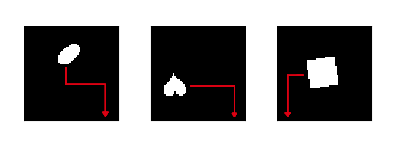
\includegraphics[scale=2]{dSprites_env}
	\end{center}
  \caption{This figure illustrates the dSprites environment, in which the agent must move all squares towards the bottom-left corner of the image and all ellipses and hearts towards the bottom-right corner of the image. The red arrows show the behaviour expected from the agent.}
   \label{fig:dSprites_env}
\end{figure}

\subsection{Agent-environment interaction} \label{ssec:env_agent_iter}

In this section, we present how all the agents introduced in the next sections interact with the environment. Each agent was trained for $N = 500K$ iterations. At the begining of a trial, the environment is reset to a random state and the agent receives an observation $o_t$. Using $o_t$, the agent select an action $a_t$, which is then executed in the environment. This lead the agent to receive a new obervation $o_{t+1}$, a reward $r_{t+1}$ and a boolean $done$ describing whether the trial is over or not. Then, the new experience ($o_t$, $a_t$, $o_{t+1}$, $r_{t+1}$, $done$) is added to the replay buffer, from which a batch is sampled to train the various neural networks of the agent. Finally, if the trial has ended, then the environment is reset to a random state leading to a new observation $o_t$, otherwise $o_{t+1}$ becomes the new $o_t$ closing the action-perception cycle. Algorithm \ref{algo:ap_cycles} summarises the agent-environment interaction.

\begin{algorithm}[H]
\label{algo:ap_cycles}
\SetAlgoLined\DontPrintSemicolon
\SetKwInOut{Input}{Input}
\SetKwFor{RepTimes}{repeat}{times}{end}
\SetAlgoLined
\Input{$env$ the environment,\\
       $agent$ the agent,\\
       $buffer$ the replay buffer,\\
       $N$ the number of training iterations.
}
 {\color{white}space}\;
$o_t$ = env.reset() \tcp*{Get the initial observation from environment}
 \RepTimes{$N$} {
   $a_t \leftarrow $ select\_action($o_t$) \tcp*{Select an action}
   $o_{t+1}, r_{t+1}, done \leftarrow $ env.execute($a_t$) \tcp*{Execute the action in the environment}
   buffer.push\_new\_experience($o_t$, $a_t$, $o_{t+1}$, $r_{t+1}$, $done$) \tcp*{Add the experience to the replay buffer}
   agent.learn(buffer) \tcp*{Perform one iteration of training}
   \eIf{done == True}{
      $o_t \leftarrow$ env.reset() \tcp*{Reset the environment when a trial ends}
   } {
      $o_t \leftarrow o_{t+1}$
   }
 }
 \caption{The interaction between the agent and the environment.}
\end{algorithm}

\subsection{Variational auto-encoder} \label{ssec:VAE}

In this section, we present our first agent based on a variational auto-encoder. The agent is composed of two deep neural networks, i.e., an encoder and a decoder. The encoder $\mathcal{E}_{\phi_s}$ takes as input an image $o_t$ and outputs the parameters of the variational posterior $Q_{\phi_s}(s_t) = \mathcal{N}(s_t;\mu,\sigma)$, where $\mu$ is the mean vector of the Gaussian distribution, and $\sigma$ are the diagonal elements of the covariance matrix. The decoder $\mathcal{D}_{\theta_o}$ models the likelihood mapping $P_{\theta_o}(o_t|s_t)$, which attributes a probability to each image $o_t$ given a state $s_t$, and is defined as:
\begin{align*}
P_{\theta_o}(o_t|s_t) = \MultiBernoulli(o_t;\hat{o}_t),
\end{align*}
where $\hat{o}_t = \mathcal{D}_{\theta_o}(s_t)$ are the values predicted by the decoder, and $\MultiBernoulli(o_t;\hat{o}_t)$ is a product of Bernoulli distributions defined as:
$$\MultiBernoulli(o_t;\hat{o}_t) = \prod_{x,y} \text{Bernoulli}(o_t[x,y];\hat{o}_t[x,y]),$$
where $\text{Bernoulli}(\,\bigcdot\,;\,\bigcdot\,)$ is a Bernoulli distribution over the possible values of the pixel $o_t[x,y]$, parameterized by the parameter $\hat{o}_t[x,y]$, which is predicted by the decoder network. The goal of the agent is to minimise the variational free energy (VFE):
$$\bm{F} = \kl{Q_{\phi_s}(s_t)}{P_{\theta_o}(o_t,s_t)} = \kl{Q_{\phi_s}(s_t)}{P_{\theta_o}(o_t|s_t)P(s_t)},$$
where $P(s_t) = \mathcal{N}(s_t; 0, I)$ is an isotropic (multivariates) Gaussian with variance one. The VFE can be re-arranged as follows:
$$\bm{F} = \kl{Q_{\phi_s}(s_t)}{P(s_t)} - \mathbb{E}_{Q_{\phi_s}(s_t)}[\ln P_{\theta_o}(o_t|s_t)],$$
where the KL-divergence between two Gaussian distributions can be computed using an analytical solution, and the expectation of the logarithm of $P_{\theta_o}(o_t|s_t)$ is approximated by a Monte-Carlo estimate using a single sample $\hat{s}_t \sim Q_{\phi_s}(s_t)$. The sample $\hat{s}_t$ is obtained using the reparameterisation trick as follows: $\hat{s}_t = \mu + \sigma \odot \hat{\epsilon}$, where $\odot$ is an element-wise product between two vectors, and $\hat{\epsilon} \sim \mathcal{N}(\epsilon;0,I)$.

To sum up, this agent takes random actions, and stores its experiences in a queue (c.f. Section \ref{ssec:env_agent_iter}). Then, batches of experiences ($o_t$, $a_t$, $o_{t+1}$, $r_{t+1}$, $done$) are sampled from the queue. The observations at time step $t$ are then fed into the encoder, which outputs the mean and log variance of a Gaussian distribution $Q_{\phi_s}(s_t) = \mathcal{N}(s_t;\mu, \sigma)$. A latent state is sampled from $Q_{\phi_s}(s_t)$ using the re-parameterisation trick, and is then prodived as input to the decoder which outputs the parameters of Bernouilli distributions $\hat{o}_t$. The KL-divergence between $Q_{\phi_s}(s_t)$ and $P(s_t)$ is computed analytically, and the logarithm of $P_{\theta_o}(o_t|s_t)$ reduces to the binary cross entropy (BCE) because $P_{\theta_o}(o_t|s_t)$ is a product of Bernouilli distributions. Next, the VFE is obtained by substracting the BCE to the KL-divergence, and back-propagation is used to update the weights of the encoder and decoder networks. Figure \ref{fig:VAE} illustrates the VAE agent presented in this section.

\begin{figure}[h]
	\begin{center}
	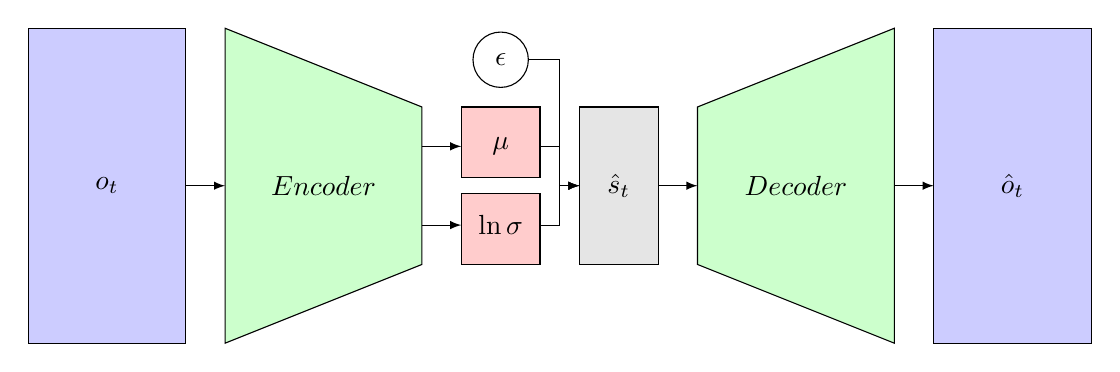
\begin{tikzpicture}[square/.style={regular polygon,regular polygon sides=4}]
		\pic{vae=$o_t$/$\mu$/$\ln \sigma$/$\hat{s}_t$/$\hat{o}_t$};
    \end{tikzpicture}

	\end{center}
  \caption{This figure illustrates the VAE agent. From left to right, we have the input image $o_t$, the encoder network, the layer of mean $\mu$ and log variance $\ln \sigma$, the epsilon random variable used for the reparameterisation trick, the latent state $\hat{s}_t$, the decoder network, and finally, the reconstructed image $\hat{o}_t$. Note, this agent takes random actions.}
   \label{fig:VAE}
\end{figure}

\subsection{Deep hidden Markov model} \label{ssec:HMM}

In this section, we present our second agent based on a hidden Markov model. Similarly to the VAE agent, the HMM agent is composed of an encoder network modelling $Q_{\phi_s}(s_\tau)$, and a decoder network modelling $P_{\theta_o}(o_\tau|s_\tau)$. However, the prior over the hidden states at time step $t+1$ depends on the hidden states and action at time step $t$. This prior is modelled by the transition network $\mathcal{T}_{\theta_s}$that predicts the parameters of the Gaussian distribution $P_{\theta_s}(s_{t+1}|s_t,a_t) = \mathcal{N}(s_{t+1}; \mathring{\mu}, \mathring{\sigma})$, where $\mathring{\mu}$ is the mean of the Gaussian distribution, and $\mathring{\sigma}$ are the diagonal elements of the covariance matrix. Recall, that the goal of the inference process is to fit the approximate posterior $Q_{\phi_s}(s_t)$ to the true posterior $P(s_t|o_{0:t})$, where $o_{0:t} = \{o_0, \hdots, o_t\}$ is the set of all observations up to the current time step $t$. Formally, this optimisation can be written as the minimization of the Kullback-Leibler divergence between the approximate and the true posterior, i.e.,
\begin{align*}
Q^*(s_t) &= \argmin_{Q_{\phi_s}(s_t)} \kl{Q_{\phi_s}(s_t)}{P(s_t|o_{0:t})}.
\end{align*}
Using a derivation almost identical to the one presented in Section \ref{ssec:derive_vfe_in_fountas}, the VFE can be proven to be:
\begin{align}
Q^*_{\phi_s}(s_t)\,\, &= \argmin_{\quad Q_{\phi_s}(s_t) \quad }\underbrace{\kl{Q_{\phi_s}(s_t)}{P_{\theta_o}(o_t|s_t)P_{\theta_s}(s_t|s_{t-1},a_{t-1})}}_{\text{variational free energy}}\label{eq:vfe_defi}\\
&= \argmin_{\quad Q_{\phi_s}(s_t)\quad } \kl{Q_{\phi_s}(s_t)}{P_{\theta_s}(s_t|s_{t-1},a_{t-1})} - \mathbb{E}_{Q_{\phi_s}(s_t)}[P_{\theta_o}(o_t|s_t)].\nonumber
\end{align}
The VFE can be computed in a similar way than for the VAE agent. Put simply, this agent takes random actions, and stores its experiences in a queue (c.f. Section \ref{ssec:env_agent_iter}). Then, batches of experiences ($o_{t-1}$, $a_{t-1}$, $o_t$, $r_t$, $done$) are sampled from the queue. The observations at time step $t - 1$ are feed into the encoder, which outputs the mean and log variance of a Gaussian distribution $Q_{\phi_s}(s_{t-1}) = \mathcal{N}(s_{t-1};\mu, \sigma)$. A latent state is sampled from $Q_{\phi_s}(s_{t-1})$ using the re-parameterisation trick, and is then prodived as input to the transition network along with action $a_{t-1}$. The transition network outputs the parameters of the Gaussian distributions $P_{\theta_s}(s_t|s_{t-1},a_{t-1}) = \mathcal{N}(s_t;\mathring{\mu}, \mathring{\sigma})$. Additionally, the observations at time step $t$ can be fed into the encoder to get the parameters of $Q_{\phi_s}(s_t) = \mathcal{N}(s_t;\hat{\mu}, \hat{\sigma})$. Sampling from $Q_{\phi_s}(s_t)$ using the reparameterisation trick gives a state $\hat{s}_t$ that when given as input of the decoder produces the parameters of a product of Bernoulli distributions $\hat{o}_{t+1}$. The KL-divergence between $Q_{\phi_s}(s_t)$ and $P_{\theta_s}(s_t|s_{t-1},a_{t-1})$ is computed analytically, and the logarithm of $P_{\theta_o}(o_t|s_t)$ reduces to the BCE because $P_{\theta_o}(o_t|s_t)$ is a product of Bernouilli distributions. Next, the VFE is obtained by substracting the BCE to the KL-divergence, and back-propagation is used to update the weights of the encoder, decoder and transition networks. Figure \ref{fig:HMM} illustrates the HMM agent. 

\begin{figure}[h]
	\begin{center}
	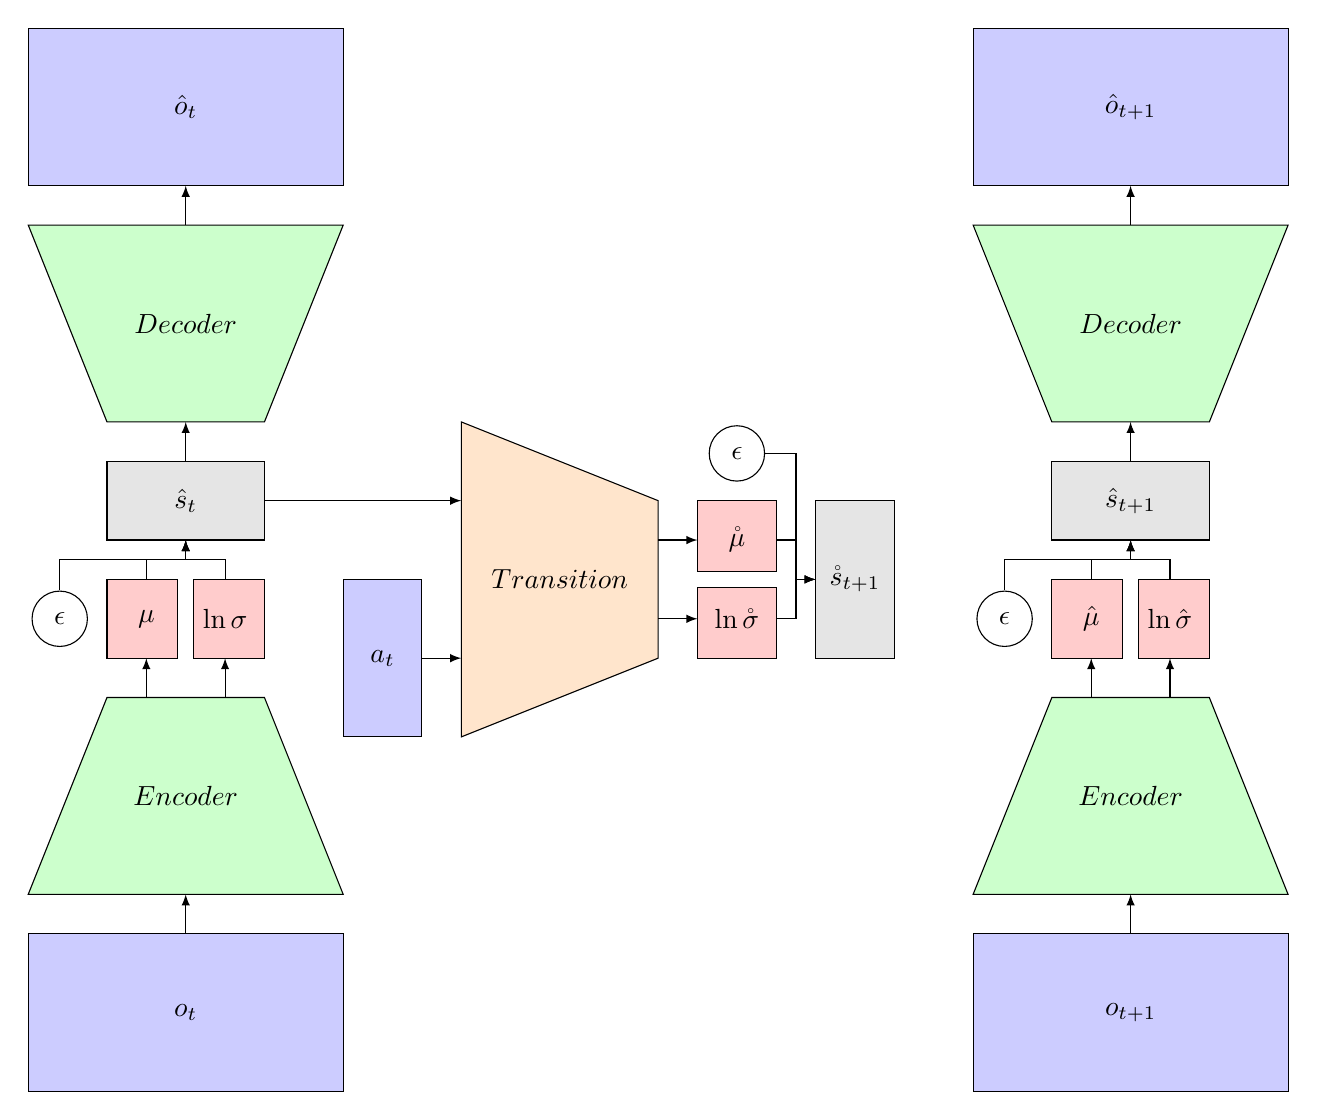
\begin{tikzpicture}
		\pic{hmm};
    \end{tikzpicture}
	\end{center}
	\caption{This figure illustrates the HMM agent. On the left and right, one can see two auto-encoders, i.e., one at time step $t$ and one at time step $t+1$. In the middle, the transition network takes as input the state and action at time $t$, i.e., $(\hat{s}_t, a_t)$, and outputs the mean $\mathring{\mu}$ and log variance $\ln\mathring{\sigma}$ of a Gaussian distribution. By sampling the latent variable $\epsilon$, and using the reparameterisation trick, we get the latent state outputed by the transition network: $\mathring{s}_{t+1} = \mathring{\mu} + \mathring{\sigma} \odot \hat{\epsilon}$ where $\hat{\epsilon}$ is sampled from a Gaussian distribution with mean zero and variance one. Importantly, the model seems to be composed of two disconnected parts, however, the variational free energy will have a complexity term between the Gaussian distributions outputed by the transition network and encoder at time $t+1$. Note, this agent takes random actions.}
   \label{fig:HMM}
\end{figure}

\subsection{Deep critical HMM} \label{ssec:CHMM}

In this section, we present our third agent that incorporates a critic network to the deep HMM presented in the previous section. The resulting model is called a deep CHMM and is illustrated in Figure \ref{fig:CHMM}. The CHMM is equipped with an encoder $\mathcal{E}_{\phi_s}$ modelling $Q_{\phi_s}(s_\tau)$, a decoder $\mathcal{D}_{\theta_o}$  modelling $P_{\theta_o}(o_\tau|s_\tau)$, a transition network $\mathcal{T}_{\theta_s}$ modelling $P_{\theta_s}(s_t|s_{t-1},a_{t-1})$, and a critic network $\mathcal{G}_{\theta_a}$ that predicts the expected free energy (see below) of each action. The critic is then used to define the prior over actions as: $P_{\theta_a}(a_t|s_t) = \sigma[-\zeta \mathcal{G}_{\theta_a}(s_t,\bigcdot\,)]$, where $\zeta$ is the precision of the prior over actions, and $\mathcal{G}_{\theta_a}(s_t,\bigcdot\,)$ is the EFE of taking each action in state $s_t$ as predicted by the critic. The encoder, decoder and transition networks are all trained like before to minimise the VFE. The critic however is trained to minimise the smooth L1 norm between its output $\mathcal{G}_{\theta_a}(s_t,\bigcdot\,)$ and the target G-values $y(\,\bigcdot\,)$, i.e., the critic minimises $\text{SL1}[\mathcal{G}_{\theta_a}(s_t,\bigcdot\,), y(\,\bigcdot\,)]$. Note, the SL1 was picked because it is less sensitive to outliers than the MSE, and the target G-values are defined as:
$$y(a_t) = G_{t+1}(a_t) + \gamma \mathbb{E}_{Q_{\phi_s}(s_{t+1})}\Big[ \max_{a_{t+1} \in \mathcal{A}} \hat{\mathcal{G}}_{\hat{\theta}_a}(s_{t+1}, a_{t+1})\Big],$$
where $Q_{\phi_s}(s_{t+1})$ can be computed by feeding the image $o_{t+1}$ sampled from the queue as input to the encoder, $G_{t+1}(a_t)$ is the expected free energy receive at time $t+1$ after taking action $a_t$ (see below), and $\gamma$ is a discount factor. Also, as for the DQN agent, we improved the training stability by implementing a target network $\hat{\mathcal{G}}_{\hat{\theta}_a}$, which is structurally identical to the critic and whose weights are syncronised with the weights of the critic every $K$ (learning) iterations. The last question to answer before to dive into the subject of the EFE is: how does the CHMM selects the action to be performed in the environment?

There are at least four possibilities that comes to mind: (i) select a random action (ii) selecting the action that maximises EFE according to the critic, i.e., $a_t^* = \argmax_{a_t} \mathcal{G}_{\theta_a}(s_t,a_t)$ (iii) sampling an action from a softmax function of the output of the critic, i.e., $a_t^* \sim \sigma[\mathcal{G}_{\theta_a}(s_t,\bigcdot\,)]$ where $\sigma[\,\bigcdot\,]$ is a softmax function, and (iv) by using the $\mathring{\epsilon}$-greedy algorithm with exponential decay, i.e., select a random action with probabilty $\mathring{\epsilon}$ or select the best action with probability $1 - \mathring{\epsilon}$ where $\mathring{\epsilon}$ starts with a high value and decay exponentially fast.

\begin{figure}[h]
	\begin{center}
	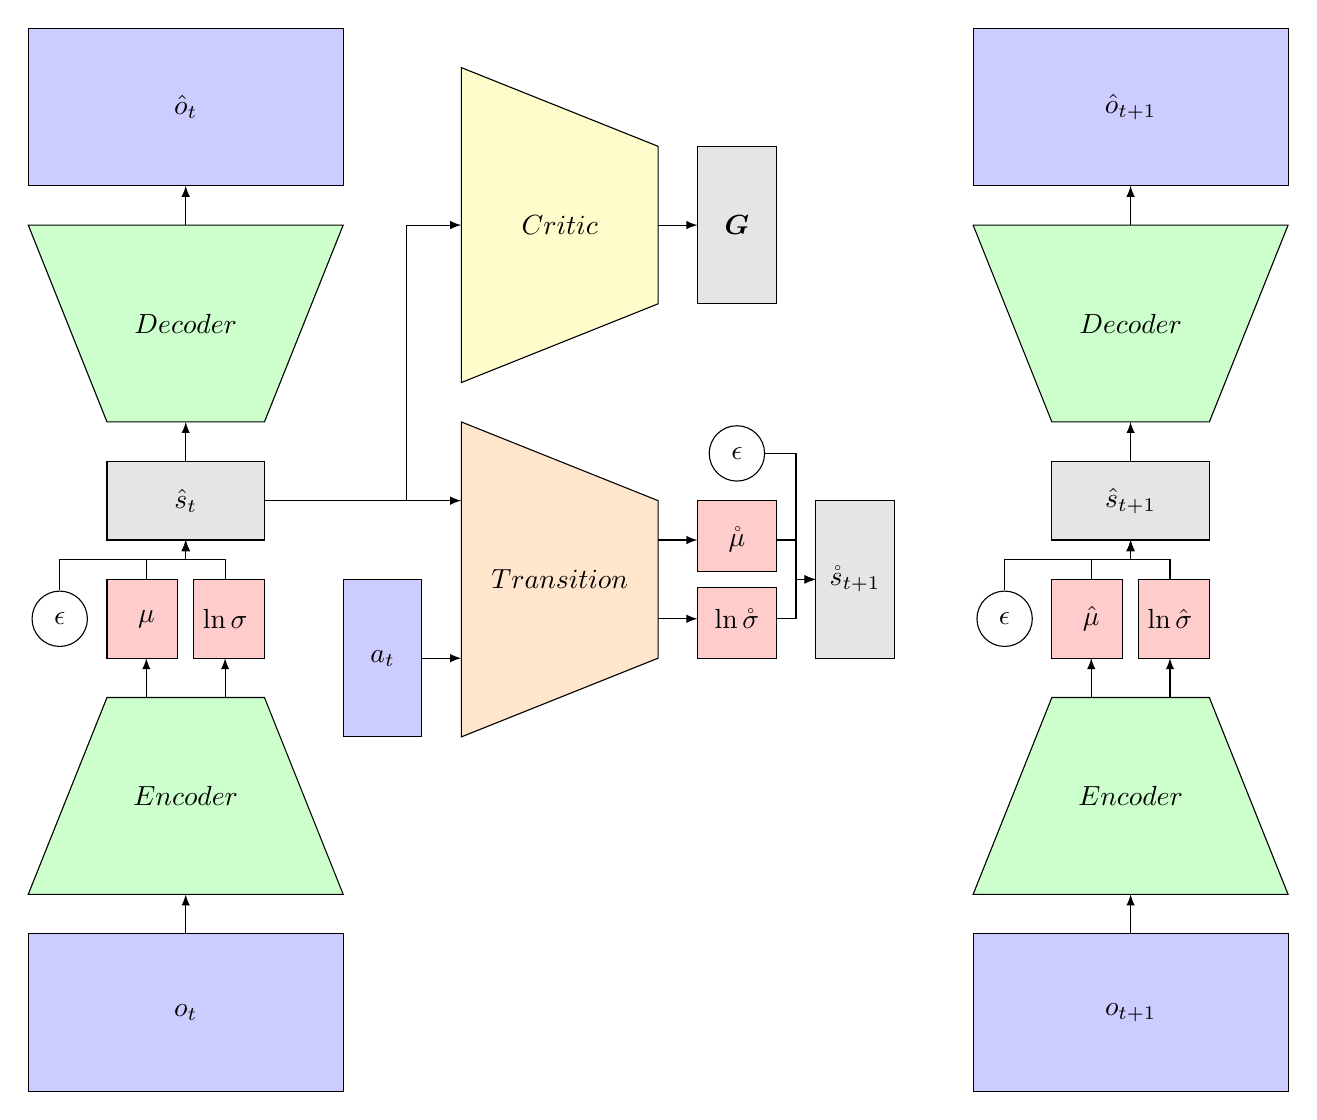
\begin{tikzpicture}[square/.style={regular polygon,regular polygon sides=4}]
		\coordinate (A) at (13.5,8);
		\coordinate (B) at (16,9);
		\coordinate (C) at (16,11);
		\coordinate (D) at (13.5,12);
		\draw[fill=yellow!20!white] (A) -- coordinate[pos=.6] (AB) (B)--(C)
         --coordinate[pos=.45] (CD) (D)
         --coordinate[pos=.55] (DA) cycle;
	    \node at (14.75, 10) {$Critic$};

		\draw[-latex] (11,6.5) -- (12.8,6.5) -- (12.8,10) -- (13.5,10);
		\draw[-latex] (16, 10) -- (16.5, 10);
		
		\draw[fill=gray!20!white] (16.5,9) rectangle (17.5,11);
	    \node at (17, 10) {$\bm{G}$};

		\pic{hmm};
    \end{tikzpicture}
	\end{center}
  \caption{This figure illustrates the CHMM agent. The only new part is the critic network, which takes as input the hidden state at time $t$ and ouputs the expected free energy of each action $\bm{G}$. Importantly, the CHMM takes actions based on the EFE.}
   \label{fig:CHMM}
\end{figure}

\subsubsection{Expected free energy} \label{ssec:efe}

In this section, we discuss the definition of the expected free energy (EFE) before to investigate various way to implement it in the context of deep active inference. Originally, the expected free energy was defined as:
\begin{align}
G(\pi) = \sum_{\tau = t+1}^T G_\tau(\pi) = \sum_{\tau = t+1}^T \mathbb{E}_{P(o_\tau|s_\tau)Q(s_\tau | \pi)}\big[\ln Q(s_\tau | \pi) - \ln P(o_\tau, s_\tau)\big],\label{eq:efe_definition}
\end{align}
where $P(o_\tau|s_\tau)$ is the likelihood mapping, $Q(s_\tau | \pi)$ is the variational distribution, and $P(o_\tau, s_\tau)$ is supposed to be the generative model but is better understood as a target distribution encoding the prior preferences of the agent. Indeed, assuming the standard generative model of active inference (i.e., a partially observable Markov decision process), the hidden states $s_\tau$ should depends on $s_{\tau-1}$ and $a_{\tau-1}$. While this remark holds for the tabular case of active inference, it is even more prevalent for the deep learning case where the VFE is defined as \eqref{eq:vfe_defi}. This remark asks whether $P(o_\tau, s_\tau)$ is really the generative model, and therfore whether the expected free energy is really the expectation of the variational free energy. Additionally, we need to arrange the definition of the EFE stated in \eqref{eq:efe_definition} to allow rewards to be incorporated:
\begin{align}
G_\tau(\pi) &= \mathbb{E}_{P(o_\tau|s_\tau)Q(s_\tau | \pi)}\big[\ln Q(s_\tau | \pi) - \ln P(o_\tau, s_\tau)\big]\nonumber\\
&= \mathbb{E}_{P(o_\tau|s_\tau)Q(s_\tau | \pi)}\big[\ln Q(s_\tau | \pi) - \ln P(s_\tau|o_\tau)- \ln P(o_\tau)\big]\nonumber\\
&\approx \mathbb{E}_{P(o_\tau|s_\tau)Q(s_\tau | \pi)}\big[\ln Q(s_\tau | \pi) - \ln Q(s_\tau)- \ln P(o_\tau)\big]\nonumber\\
&= \underbrace{\kl{Q(s_\tau | \pi)}{Q(s_\tau)}}_{\text{epistemic value}} - \underbrace{\mathbb{E}_{P(o_\tau|s_\tau)Q(s_\tau | \pi)}\big[\ln P(o_\tau)\big]}_{\text{extrinsic value}},\label{eq:efe_practice}
\end{align}

\subsubsection{A principled estimate of the EFE at time $t + 1$?}

Now, the question is how to estimate \eqref{eq:efe_practice}, and we focus on the case where $\tau = t + 1$. Note, because $\tau = t+1$, the policy $\pi$ contains only one action $a_t$, i.e., $\pi = a_t$. In the tabular version of active inference, the variational distribution is composed of a factor $Q(s_\tau | \pi)$. However, in the deep active inference literature, the variational distribution does not contains such factor. Generally, a Monte-Carlo estimates is used as follows:
\begin{align}
Q(s_{t+1} | a_t) = \mathbb{E}_{Q_{\phi_s}(s_t)}\big[P_{\theta_s}(s_{t+1}|s_t, a_t)\big] \approx \frac{1}{N} \sum_{i = 1}^N P_{\theta_s}(s_{t+1}|s_t = \hat{s}_t, a_t), \label{eq:vd_or_gm}
\end{align}
where $\hat{s}_t \sim Q_{\phi_s}(s_t)$. Importantly, for the expected free energy to be the expectation of the variational free energy $Q(s_{t+1} | a_t)$ should be a factor of the variational distribution. However, \eqref{eq:vd_or_gm} is estimated using a factor of the generative model $P_{\theta_s}(s_{t+1}|s_t = \hat{s}_t, a_t)$. This is a conceptual problem of current deep active inference approaches. 
In what follows, we use $N=1$ leading to a simplified version of the estimate:
\begin{align}
Q(s_{t+1} | a_t) \approx P_{\theta_s}(s_{t+1}|s_t = \hat{s}_t, a_t).
\end{align}
At this point, we have an estimate for $Q(s_{t+1} | a_t)$ and $Q_{\phi_s}(s_t)$ is the variational distribution. The only missing piece of the puzzle currently is an estimate of the extrinsic value. In the tabular version of active inference, the preferences of the agent can be related to the rewards from the reinforcement learning literature. In this paper, we follow \citep{dacosta2020relationship} and define the prior preferences as:
\begin{align*}
P(o_\tau) = \frac{\exp(\psi r_\tau[o_\tau])}{\sum_{o_\tau} \exp(\psi r_\tau[o_\tau])},
\end{align*}
where $\psi$ is the precision of the prior preferences, and $r_\tau[o_\tau]$ is the reward obtained when making observation $o_\tau$. Taking the logarithm of the above equation leads to:
\begin{align}
\ln P(o_\tau) &= \psi r_\tau[o_\tau] - \ln \sum_{o_\tau} \exp(\psi r_\tau[o_\tau])\nonumber\\
&= \psi r_\tau[o_\tau] + C, \label{eq:prior_pref}
\end{align}
where we used that the summation over all $o_\tau$ is a normalisation term, i.e., a constant. Using \eqref{eq:prior_pref}, we can now create an estimate of the extrinsic value as follows:
\begin{align*}
\mathbb{E}_{P_{\theta_o}(o_\tau|s_\tau)Q(s_\tau | a_t)}\big[\ln P(o_\tau)\big] \approx \frac{1}{M} \sum_{i = 1}^M \ln P(o_\tau = \hat{o}_\tau) = \frac{1}{M} \sum_{i = 1}^M \psi r_\tau[o_\tau] + C,
\end{align*}
where $\hat{o}_\tau \sim P_{\theta_o}(o_\tau|s_\tau=\hat{s}_\tau)$ and $\hat{s}_\tau \sim Q(s_\tau | a_t)$. In what follows, we use $M=1$ and discard the constant\footnote{Removing a constant does not influence which policy is the best. Indeed, $\pi^* = \argmax_\pi G(\pi) = \argmax_\pi G(\pi) - C$.}, which leads to a simplified version of the estimate:
\begin{align*}
\mathbb{E}_{P_{\theta_o}(o_\tau|s_\tau)Q(s_\tau | a_t)}\big[\ln P(o_\tau)\big] \delequal \psi r_\tau[o_\tau] \delequal \psi r_\tau,
\end{align*}
where we simplied the notation by denoting $r_\tau[o_\tau]$ as $r_\tau$. To conclude, we have the following estimate for the EFE at time $\tau = t+1$:
\begin{align}
G_{t+1}(a_t) &\approx \kl{Q(s_{t+1} | a_t)}{Q_{\phi_s}(s_{t+1})} - \mathbb{E}_{P_{\theta_o}(O_{t+1}|s_{t+1})Q(s_{t+1} | a_t)}\big[\ln P(O_{t+1})\big]\nonumber\\
&\approx \kl{P_{\theta_s}(s_{t+1}|s_t = \hat{s}_t, a_t)}{Q_{\phi_s}(s_{t+1})} - \psi r_{t+1},
\end{align}
where $\hat{s}_t \sim Q_{\phi_s}(s_t)$, $P_{\theta_s}(s_{t+1}|s_t, a_t)$ is known from the generative model, $Q_{\phi_s}(s_{t+1})$ is known from the variational distribution, the KL-divergence can be estimated using an analytical solution, $\psi$ is a hyperparamter modulating the precision of the prior preferences, and $r_{t+1}$ is the reward obtained at time step $t+1$.

\subsubsection{Other definitions of the EFE at time $t + 1$} \label{ssec:efe_other_defe}

In the previous section, we have presented what may be a principle way to estimate the EFE. As will be discussed later in this paper, this estimate of the EFE was not very fruitful empirically. Out of curiosity, we also experimented with the following definitions:
\begin{align*}
G^1_{t+1}(a_t) &= H[Q_{\phi_s}(s_{t+1})] - H[P_{\theta_s}(s_{t+1}|s_t =\hat{s}_t, a_t)] - \psi r_{t+1},\\
G^2_{t+1}(a_t) &= H[P_{\theta_s}(s_{t+1}|s_t =\hat{s}_t, a_t)] - H[Q_{\phi_s}(s_{t+1})] - \psi r_{t+1},\\
G^3_{t+1}(a_t) &= \kl{Q_{\phi_s}(s_{t+1})}{P_{\theta_s}(s_{t+1}|s_t = \hat{s}_t, a_t)} - \psi r_{t+1},
\end{align*}
where all the entropy terms and the KL-divergence were computed analytically. Also, we experimented with simply predicting the (negative) expected future reward as follows:
\begin{align*}
G^4_{t+1}(a_t) &= - \psi r_{t+1},
\end{align*}
which is effectively making the job of the critic identical to the job of the Q-network in the DQN agent (c.f. Section \ref{ssec:dqn} for details). Except for the fact that the Q-network is taking observations as input while the critic takes hidden states. 

\subsection{Deep Active Inference} \label{ssec:DAI}

In this section, we discuss the full deep active inference (DAI) agent illustrated in Figure \ref{fig:DAI}. Put simply, this agent is composed of five deep neural networks, i.e., the encoder, the decoder, the transition, the critic and the policy network. The decoder $\mathcal{D}_{\theta_o}$ models $P_{\theta_o}(o_\tau|s_\tau)$ as a product of Bernoulli distributions, i.e., $P_{\theta_o}(o_\tau|s_\tau) = \MultiBernoulli(o_\tau;\hat{o}_\tau)$ where $\hat{o}_\tau = \mathcal{D}_{\theta_o}(s_\tau)$. The transition $\mathcal{T}_{\theta_s}$ models $P_{\theta_s}(s_{\tau+1}|s_\tau,a_\tau)$ as a Gaussian distribution, i.e., $P_{\theta_s}(s_{\tau+1}|s_\tau,a_\tau) = \mathcal{N}(s_{\tau+1}|\mathring{\mu},\mathring{\sigma})$ where $\mathring{\mu},\ln \mathring{\sigma} = \mathcal{T}_{\theta_s}(s_\tau,a_\tau)$. The critic $\mathcal{G}_{\theta_a}$ outputs a vector containing the predicted expected free energy of each action, which is used to defined the prior over action as $P_{\theta_a}(a_\tau|s_\tau) = \sigma[-\zeta \mathcal{G}_{\theta_a}(s_\tau, \bigcdot\,)]$, where $\sigma[\bigcdot]$ is a softmax function and $\zeta$ is the precision of the prior over actions. With this in mind the full generative model of the agent is:
\begin{align*}
P_{\theta}(o_{o:T}, s_{o:T}, a_{o:T-1}) = P(s_0)\prod_{\tau = 0}^T P_{\theta_o}(o_\tau|s_\tau) \prod_{\tau = 0}^{T-1} P_{\theta_s}(s_{\tau+1}|s_\tau, a_\tau) P_{\theta_a}(a_\tau|s_\tau),
\end{align*}

\begin{figure}[H]
	\begin{center}
	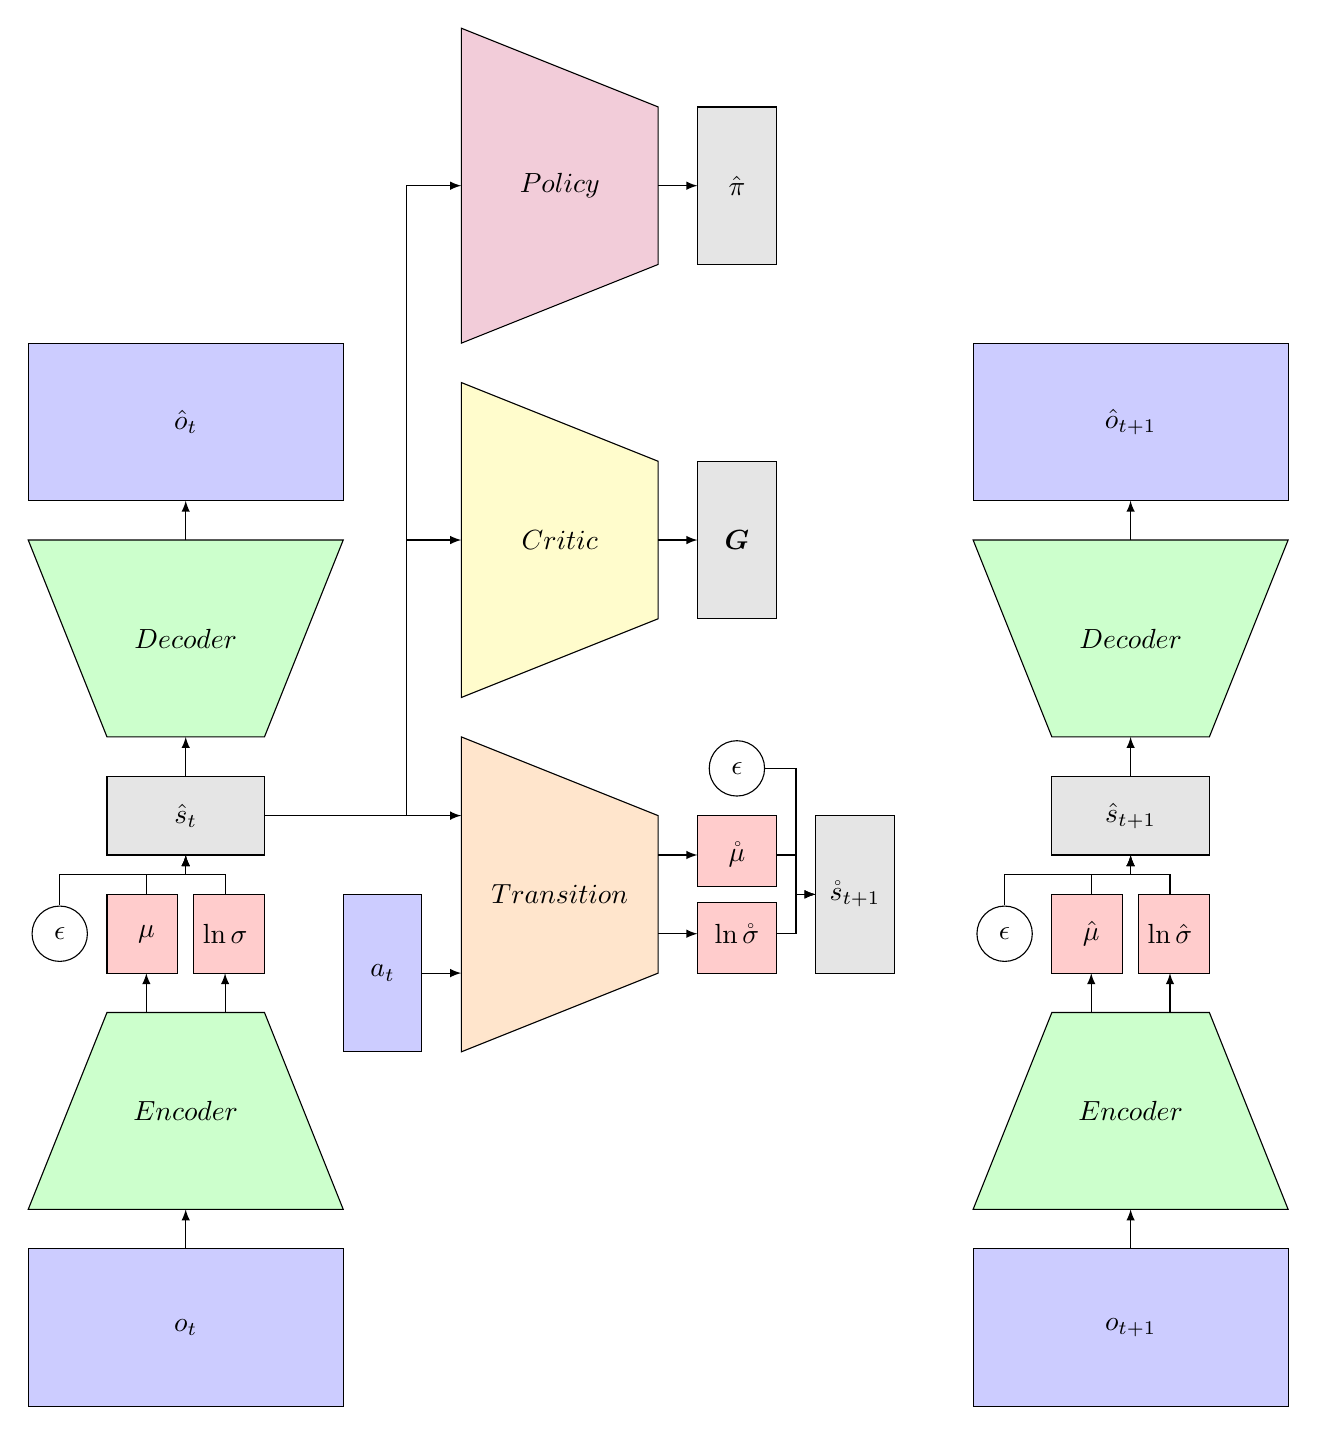
\begin{tikzpicture}[square/.style={regular polygon,regular polygon sides=4}]
		\coordinate (A) at (13.5,12.5);
		\coordinate (B) at (16,13.5);
		\coordinate (C) at (16,15.5);
		\coordinate (D) at (13.5,16.5);
		\draw[fill=purple!20!white] (A) -- coordinate[pos=.6] (AB) (B)--(C)
         --coordinate[pos=.45] (CD) (D)
         --coordinate[pos=.55] (DA) cycle;
	    \node at (14.75, 14.5) {$Policy$};
		\draw[-latex] (11,6.5) -- (12.8,6.5) -- (12.8,14.5) -- (13.5,14.5);
		\draw[-latex] (16, 14.5) -- (16.5, 14.5);
		\draw[fill=gray!20!white] (16.5,13.5) rectangle (17.5,15.5);
	    \node at (17, 14.5) {$\hat{\pi}$};


		\coordinate (A) at (13.5,8);
		\coordinate (B) at (16,9);
		\coordinate (C) at (16,11);
		\coordinate (D) at (13.5,12);
		\draw[fill=yellow!20!white] (A) -- coordinate[pos=.6] (AB) (B)--(C)
         --coordinate[pos=.45] (CD) (D)
         --coordinate[pos=.55] (DA) cycle;
	    \node at (14.75, 10) {$Critic$};

		\draw[-latex] (11,6.5) -- (12.8,6.5) -- (12.8,10) -- (13.5,10);
		\draw[-latex] (16, 10) -- (16.5, 10);
		
		\draw[fill=gray!20!white] (16.5,9) rectangle (17.5,11);
	    \node at (17, 10) {$\bm{G}$};

		\pic{hmm};
    \end{tikzpicture}
	\end{center}
  \caption{This figure illustrates the DAI agent. The only new part is the policy network, which takes as input the hidden state at time $t$ and ouputs the the parameters $\hat{\pi}$ of the variational posterior over actions. Importantly, the DAI takes actions based on the EFE.}
   \label{fig:DAI}
\end{figure}

where $P(s_0) = \mathcal{N}(s_0;\mu_0,\sigma_0)$ is a Gaussian prior over initial hidden states. Let $t$ be the present time step. The DAI agent maintains posterior beliefs over the present states $s_t$ and action $a_t$. The variational posterior over states $Q_{\phi_s}(s_t)$ is a Gaussian distribution modelled by the encoder $\mathcal{E}_{\phi_s}$, i.e., $Q_{\phi_s}(s_t) = \mathcal{N}(s_t;\mu, \sigma)$ where $\mu, \ln\sigma = \mathcal{E}_{\phi_s}(o_t)$. The variational posterior over actions $Q_{\phi_a}(a_t|s_t)$ is a categorical distribution modelled by the policy network $\mathcal{P}_{\phi_a}$, i.e., $Q_{\phi_a}(a_t|s_t) = \text{Cat}(a_t;\hat{\pi})$ where $\hat{\pi} = \mathcal{P}_{\phi_a}(s_t)$. The full variational distribution is therefore defined as:
\begin{align*}
Q_{\phi}(a_t,s_t) = Q_{\phi_a}(a_t|s_t)Q_{\phi_s}(s_t).
\end{align*}
The variational free energy of the DAI agent is derived in a similar way to the VFE of Section \ref{ssec:derive_vfe_in_fountas}, and is defined as:
\begin{align}
Q^*_{\phi}(s_t, a_t) &= \argmin_{Q_{\phi}(s_t, a_t)}\underbrace{\kl{Q_{\phi}(s_t, a_t)}{P_{\theta_o}(o_t|s_t)P_{\theta_s}(s_t|s_{t-1},a_{t-1})P_{\theta_a}(a_t|s_t)}}_{\text{variational free energy}}\label{eq:vfe_defi_dai}\\
&= \argmin_{Q_{\phi}(s_t, a_t)} \quad\,\,\, \mathbb{E}_{Q_{\phi_s}(s_t)}\big[\kl{Q_{\phi_a}(a_t|s_t)}{P_{\theta_a}(a_t|s_t)}\big] + \kl{Q_{\phi_s}(s_t)}{P_{\theta_s}(s_t|s_{t-1},a_{t-1})}\nonumber\\
&\quad\qquad\qquad - \mathbb{E}_{Q_{\phi_s}(s_t)}[\ln P_{\theta_o}(o_t|s_t)].\nonumber
\end{align}

The VFE is therefore a function of $s_{t-1}$, $a_{t-1}$, and $o_t$. Both $a_{t-1}$, and $o_t$ can be obtained from the replay buffer, and $s_{t-1}$ can sampled from the variational distribution predicted by the encoder network when observation $o_{t-1}$ provided as input. Also, the KL-divergences can be computed analytically, the expectations w.r.t $Q_{\phi_s}(s_t)$ can be approximated using a Monte-Carlo estimate, and the logarithm of the likelihhod mapping reduces to the BCE because $P_{\theta_o}(o_t|s_t)$ is a product of Bernoulli distributions. Thus, all the VFE terms can be estimated, and the encoder, decoder, transition and policy networks can be trained to minimise the VFE using gradient descent. The critic's weights are optimised as in Section \ref{ssec:CHMM} using gradient descent to minimise the smooth L1 norm between the critic's output $\mathcal{G}_{\theta_a}(s_t,\bigcdot\,)$ and the target G-values $y(\,\bigcdot\,)$, i.e., $\text{ SL1}[\mathcal{G}_{\theta_a}(s_t,\bigcdot\,), y(\,\bigcdot\,)],$ where the target G-values are defined as:
$$y(a_t) = G_{t+1}(a_t) + \gamma \mathbb{E}_{Q_{\phi_s}(s_{t+1})}\Big[ \max_{a_{t+1} \in \mathcal{A}} \hat{\mathcal{G}}_{\hat{\theta}_a}(s_{t+1}, a_{t+1})\Big],$$
where $Q_{\phi_s}(s_{t+1})$ can be computed by feeding the image $o_{t+1}$ sampled from the queue as input to the encoder, $\gamma$ is a discount factor, and $G_{t+1}(a_t)$ is the expected free energy receive at time $t+1$ after taking action $a_t$, i.e.,
\begin{align}
G_{t+1}(a_t) &\approx \kl{P_{\theta_s}(s_{t+1}|s_t = \hat{s}_t, a_t)}{Q_{\phi_s}(s_{t+1})} - \psi r_{t+1},
\end{align}
where $\hat{s}_t \sim Q_{\phi_s}(s_t)$, $\psi$ is a hyperparamter modulating the precision of the prior preferences, and $r_{t+1}$ is the reward obtained at time step $t+1$. Note, we also experimented with other definitions of the EFE at time $t + 1$ as presented in Section \ref{ssec:efe_other_defe}. Finally, we discuss how action selection is performed by the DAI agent. At least four possibilities comes to mind: (i) select a random action (ii) selecting the action with the highest posterior probability according to the policy network, i.e., $a_t^* = \argmax_{a_t} Q_{\phi_a}(a_t|s_t)$ (iii) sampling an action from the posterior over actions, i.e., $a_t^* \sim Q_{\phi_a}(a_t|s_t)$, and (iv) by using the $\mathring{\epsilon}$-greedy algorithm with exponential decay, i.e., random action with probabilty $\mathring{\epsilon}$ or best action with probability $1 - \mathring{\epsilon}$.

\section{Results} \label{sec:results}

In this section, we discuss the results obtained by the DQN agent and each model presented in Section \ref{sec:existing_research}. The code that can be used to reproduced all the experiements can be found on GitHub at the following URL: \url{https://github.com/ChampiB/Challenges_Deep_Active_Inference}. Section \ref{ssec:dqn_results} presents the results obtained by the DQN agent. Section \ref{ssec:vae_results} presents the VFE obtained by the VAE agent, and shows the reconstructed images produced by the VAE. Section \ref{ssec:hmm_results} shows the VFE of the HMM agent as well as the generated sequences of images. Section \ref{ssec:chmm_results} illustrates the VFE obtained by the CHMM as well as the reward obtained by this model when using different action selection scheme and different definition for the EFE. Finally, Section \ref{ssec:dai_results} dicusses the VFE obtained by the DAI agent, as well as the rewards obtained by this model. Note, each time CKA is used in the following sections, we sampled 5K data examples, and we used them to compute all the CKA scores. 
%TODO Section \ref{ssec:fixing_fountas} looks at what happens when fixing some of the inconsistencies between the code and the paper.


%TODO \subsection{What happens when correcting the $DAI_{MC}$ implementation?} \label{ssec:fixing_fountas}

%TODO In this section, we take a look at what happens when fixing the inconsistencies between the code and the paper of the $DAI_{MC}$ agent. The relevant code is available at the following URL: \url{https://github.com/ChampiB/fountas-deep-active-inference-mc}. The $DAI_{MC}$ agent was trained on the dSprites environment (c.f., Section \ref{ssec:dSprites_env} for details), and its performance is based on the reward obtained by the agent. Briefly, the agent receives a reward of $-1$, if it never pulls the shape through the bottom row of the image or if it does so at the antipode of the appropriate corner. As the agent pulls the shape through the bottom row closer and closer to the appropriate corner, its reward increases until reaching a maximum of $1$. The percentage of the task solved (i.e., the evaluation metric) is calculated as follows:
%TODO $$P(\text{solved}) = \frac{\text{total rewards} + \text{number of runs}}{2.0 \times \text{number of runs}}.$$
%TODO Intuitively, the numerator shifts the rewards so that they are bounded between zero and two, and the denominator renormalises the reward to give a score between zero and one. A score of zero therefore corresponds to an agent always failing to enter the bottom row or doing so at the antipode of the appropriate corner. In contrast, a score of one corresponds to an agent always entering the bottom row through the appropriate corner.

%TODO Table \ref{tab:fix_fountas} presents the results obtained when fixing some of the inconsistencies between the code en the paper. Fixing the computation of the omega parameter (for top-down attention) leads to a decrease in performance of around 20\%. Fixing the expected free energy and variational free energy does not change the performance of the agent a lot. Additionally, when fixing all three inconsistencies (i.e., expected and variational free energy and omega), the performance of the agent decreases by around 10\%.

%TODO \begin{table}
%TODO \begin{center}
%TODO \begin{tabular}{|c|c|c|c|c|}
%TODO   \hline
%TODO   Omega Fixed & VFE Fixed & EFE Fixed & $P(\text{solved})$\\ 
%TODO   \hline
%TODO   \hline
%TODO   $\times$ & $\times$ & $\times$ & 0.661 \\ 
%TODO   \hline
%TODO   $\checkmark$ & $\times$ & $\times$ & 0.469 \\ 
%TODO   \hline
%TODO   $\times$ & $\checkmark$ & $\times$ & 0.675 \\ 
%TODO   \hline
%TODO   $\times$ & $\times$ & $\checkmark$ & 0.665 \\ 
%TODO   \hline
%TODO   $\checkmark$ & $\checkmark$ & $\checkmark$ & 0.576 \\ 
%TODO   \hline
%TODO \end{tabular}
%TODO \end{center}
%TODO \caption{\label{tab:fix_fountas}
%TODO This table shows the results obtained by the $DAI_{MC}$ agent when fixing some inconsistencies that were present between the code and the paper.}
%TODO \end{table}

\subsection{DQN agent} \label{ssec:dqn_results}

In this section, we report the results obtained by the DQN agent. As shown in Figure \ref{fig:DQN_rewards}, the DQN was able to accumulate a total amount of reward of around 50K. This results support the correctness of our implementation, and give us a baseline which can be used to evaluate the performance of the CHMM and DAI agents. To better understand the representations learned by a DQN, we compute the CKA scores between the activations of its layers. We can see in Figure~\ref{fig:cka-dqn} that while the layers closer to the input retains some similarity with each others, the last two layers learn highly specific representations.


\begin{figure}[H]
	\begin{center}
		\begin{tikzpicture}[square/.style={regular polygon,regular polygon sides=4}, scale=0.75]
	    \node at (0, 0) {\includegraphics[scale=0.3]{dqn_rewards}};
	    \node[gray!60!black,rotate=90] at (-9.2, 0.3) {Total Rewards};
	    \node[gray!60!black] at (0, -4.4) {Training Iterations};
	\end{tikzpicture}
	\end{center}
   \caption{This figure illustrates the cumuated rewards obtained by the DQN agent during the 500K training iterations.}
   \label{fig:DQN_rewards}
\end{figure}

\begin{figure}[H]
    \centering
    \includegraphics[width=0.5\linewidth]{cka_figures/CKA_dqn_1_dqn_1}
    \caption{We can see that the first three layers of the DQN learn very similar representations (CKA is close to 1).
    The representations learned by the fourth layer starts to diverge (CKA is lower), and the last two layers learn
    highly specific representations which are very different from the previous layers (CKA is close to 0) but slightly similar to each other}\label{fig:cka-dqn}
\end{figure}

\subsection{VAE agent} \label{ssec:vae_results}

In this section, we report the results obtained by the VAE agent. As shown in Figure \ref{fig:VAE_vfe}, the VFE decreases as training progresses. Also, at the end of the 500K training iterations, the VAE is able to properly reconstruct the  image, c.f., Figure \ref{fig:VAE_reconstruction}. Additionally, since the VAE takes random actions in the environment, the agent was unable to solve the task and accumulated a total amount of reward of around -7K. Those results support the correctness of our implementation, and give us a baseline for the amount of rewards obtained under random play in the dSprites environment.

To observe the representations learned by VAEs, we compute the CKA scores between the activations of the different layers of the encoder. We can see in Figure~\ref{sfig:cka-vae-vae} that the representations are strongly similar between all layers, with the exception the mean and variance representations, similarly to what was observed in~\citet{Bonheme2022}. As illustrated in Figure~\ref{sfig:cka-vae-dqn}, these representations are generally similar to those learned by DQN in early layers but the representations of the last two layers strongly differ, reflecting the difference of learning objectives between VAE and DQN.

\begin{figure}[H]
	\begin{center}
	\begin{tikzpicture}[square/.style={regular polygon,regular polygon sides=4}, scale=0.75]
	    \node at (0, 0) {\includegraphics[scale=0.4]{vae_vfe}};
	    \node[gray!60!black,rotate=90] at (-7.6, 0) {VFE};
	    \node[gray!60!black] at (0, -5.8) {Training Iterations};
	\end{tikzpicture}
	\end{center}
   \caption{This figure illustrates the variational free energy of the VAE agent during the 500K iterations of training.}
   \label{fig:VAE_vfe}
\end{figure}

\begin{figure}[H]
	\begin{center}
	\includegraphics[scale=0.6]{vae_reconstruction}
	\end{center}
   \caption{This figure illustrates the reconstructed image produced by the VAE after 500K training iterations. The columns alternates between the input images and the reconstructed images.}
   \label{fig:VAE_reconstruction}
\end{figure}

\begin{figure}[ht!]
    \centering
    \begin{subfigure}{.4\textwidth}
        \centering
        \includegraphics[draft=false,width=\linewidth]{cka_figures/CKA_vae_1_vae_1}
        \caption{}\label{sfig:cka-vae-vae}
    \end{subfigure}%
    \begin{subfigure}{.4\textwidth}
        \centering
        \includegraphics[draft=false,width=\linewidth]{cka_figures/CKA_dqn_1_vae_1}
        \caption{}\label{sfig:cka-vae-dqn}
    \end{subfigure}
    \caption{(a) shows the similarity between the representations learned by different layers of the encoder of a VAE.
        (b) shows the similarity between the representations learned by a DQN and a VAE.}
    \label{fig:cka-vae}
\end{figure}

\subsection{HMM agent} \label{ssec:hmm_results}

In this section, we report the results obtained by the HMM agent. As shown in Figure \ref{fig:HMM_vfe}, the VFE decreases as training progresses. By comparing Figure \ref{fig:VAE_vfe} and \ref{fig:HMM_vfe}, one can see that the HMM has a lower VFE than the VAE. This is because the agent has more flexibility regarding the prior, i.e., the log-likelihood is the same between the two models but the complexity terms is smaller for the HMM than for the VAE. Also, at the end of the 500K training iterations, the HMM is able to properly generate sequence of images, c.f., Figure \ref{fig:HMM_reconstruction}. Additionally, since the HMM takes random actions in the environment, the agent was unable to solve the task and accumulated a total amount of reward of around -7K. Those results support the correctness of our implementation, and comfirm our baseline for the amount of rewards obtained under random play in the dSprites environment.

Similarly to VAEs, we are interested in observing the representations learned by the encoder of the HMM, but also by its transition network. The representations learned by the encoder of the HMM follows the same trend as those learned by VAEs with an even more marked dissimilarity between the log variance of the HMM an the other representations learned by this model, as illustrated in Figures~\ref{sfig:cka-hmm-hmm} and~\ref{sfig:cka-hmm-vae}. We can further observe in Figure~\ref{sfig:cka-hmm-hmm} that the transition network learns representations similar to the mean representation in its first three layers, while the representations learned by the last layer are not similar to any other representations learned by the transition or encoder networks. We can also see in Figure~\ref{sfig:cka-hmm-vae} that the mean and variance representations learned by HMM are different from those learned by VAEs, possibly indicating that the transition network influences these two representations. Similarly to VAEs, one can observe in Figure~\ref{sfig:cka-hmm-dqn}, that the representations learned by the encoder of the HMM are close to those of the DQN in the first layers but very different in the last two layers, with a stronger dissimilarity between the log variance of the HMM and the representations of the DQN.

\begin{figure}[H]
	\begin{center}
	\begin{tikzpicture}[square/.style={regular polygon,regular polygon sides=4}, scale=0.75]
	    \node at (0, 0) {\includegraphics[scale=0.56]{hmm_vfe}};
	    \node[gray!60!black, rotate=90] at (-8.2, 0) {VFE};
	    \node[gray!60!black] at (0, -5.8) {Training Iterations};
	\end{tikzpicture}
	\end{center}
   \caption{This figure illustrates the variational free energy of the HMM agent during the 500K iterations of training.}
   \label{fig:HMM_vfe}
\end{figure}

\begin{figure}[H]
	\begin{center}
	\includegraphics[scale=0.4]{hmm_reconstruction}
	\end{center}
   \caption{This figure illustrates the sequences of reconstructed images generated by the HMM after 500K training iterations. The columns alternates between the ground truth images and the reconstructed images. Time passes vertically (from top to bottom), and within each column the same action is executed repeatedly.}
   \label{fig:HMM_reconstruction}
\end{figure}

\begin{figure}[ht!]
    \centering
    \begin{subfigure}{.3\textwidth}
        \centering
        \includegraphics[draft=false,width=\linewidth]{cka_figures/CKA_hmm_1_hmm_1}
        \caption{}\label{sfig:cka-hmm-hmm}
    \end{subfigure}%
    \begin{subfigure}{.3\textwidth}
        \centering
        \includegraphics[draft=false,width=\linewidth]{cka_figures/CKA_hmm_1_vae_1}
        \caption{}\label{sfig:cka-hmm-vae}
    \end{subfigure}%
    \begin{subfigure}{.3\textwidth}
        \centering
        \includegraphics[draft=false,width=\linewidth]{cka_figures/CKA_dqn_1_hmm_1}
        \caption{}\label{sfig:cka-hmm-dqn}
    \end{subfigure}
    \caption{(a) shows the similarity between the representations learned by different layers of the encoder and transition network of an HMM.
        (b) shows the similarity between the representations learned by an HMM and a VAE.
        (c) shows the similarity between the representations learned by a DQN and an HMM.}
    \label{fig:cka-hmm}
\end{figure}

\subsection{CHMM agent} \label{ssec:chmm_results}

In this section, we report the results obtained by the CHMM agent, when using different action selection strategies and different definitions of the expected free energy. Figure \ref{fig:CHMM_rewards_eg} presents the cumulated rewards obtained by the CHMM agents using an $\mathring{\epsilon}$-greedy algorithm for action selection, as well as the total rewards obtained by the DQN agent. The critic network of the CHMM agents were trained to predict the five definitions of the expected free energy proposed in Section \ref{ssec:CHMM}. Note, the DQN agent performs better that any of the CHMM agents, and the only agent that solves the task is the CHMM maximising reward only, i.e., without any information gain. Figure \ref{fig:CHMM_rewards_s} presents the same experiement as Figure \ref{fig:CHMM_rewards_eg} except that the CHMM agents were using softmax sampling for action selection. In this setting, none of the CHMM agents were able to solve the task. Finally, Figure \ref{fig:CHMM_rewards_b} presents yet again the same experiements but this time the CHMM agents were selecting the best action according to the critic. In this setting, only the CHMM maximising reward was able to solve the task. Also, by comparing Figures \ref{fig:CHMM_rewards_eg} and \ref{fig:CHMM_rewards_b}, it becomes clear that the CHMM using an $\mathring{\epsilon}$-greedy algorithm performs better than the CHMM selecting the best action according to the critic. Put simply, the latter suffers from a lack of exploration that slows down its learning. 

Additionally, Figure \ref{fig:CHMM_vfe} represents the variational free energy of the CHMM agent using the $\mathring{\epsilon}$-greedy algorithm. All the agents were able to minimise their variational free energy, except the one displayed in orange who crashed; this agent was minimising the expected free energy as defined by $G^1$. Note, $G^1$ is neither the reward nor the ``principled" expected free energy, i.e., $G^1$ is one of definitions that we experiemented with out of curiosity. Also, the variational free energy of the CHMM agents using softmax sampling and best action selection are not presented in this paper, because their results are very similar to the results shown in Figure \ref{fig:CHMM_vfe}.

Finally, Figure \ref{fig:CHMM_reconstruction} shows examples of predicted trajectories after the CHMM was trained. By comparing with Figure    \ref{fig:HMM_reconstruction}, we see that the CHMM does not understand the dynamics of the environment as well as the HMM agent. This sugguests a conflit between the two goals of the agent, i.e., maximising reward (or expected free energy) and learning a model of the world. More precisely, Figure \ref{fig:HMM_reconstruction} shows that a HMM agent taking random actions is able to gather a large diversity of training examples and learns the dynamic of the environment beautifully, but does not solve the task. In contrast, the CHMM maximising reward solves the task but learns a poor model of the environment, c.f., Figure \ref{fig:CHMM_reconstruction}.

\begin{figure}[H]
	\begin{center}
	\includegraphics[scale=0.3]{chmm_rewards_eg.png}
	\end{center}
   \caption{This figure illustrates the total amount of rewards gathered by the CHMM agents (with $\mathring{\epsilon}$-greedy action selection) during the 500K iterations of training. The only two models that were able to solve the task are the ones maximising rewards (without information gain), i.e., the DQN agent in red and the CHMM whose critic network was predicting reward only in gray.}
   \label{fig:CHMM_rewards_eg}
\end{figure}

\begin{figure}[H]
	\begin{center}
		\includegraphics[scale=0.3]{chmm_rewards_s.png}
	\end{center}
   \caption{This figure illustrates the total amount of rewards gathered by the CHMM agents (with softmax sampling) during the 500K iterations of training. The only model that was able to solve the task is the DQN agent in red, and all CHMM agents failed.}
   \label{fig:CHMM_rewards_s}
\end{figure}

\begin{figure}[H]
	\begin{center}
	    \includegraphics[scale=0.3]{chmm_rewards_b.png}
	\end{center}
   \caption{This figure illustrates the total amount of rewards gathered by the CHMM agents (with best action selection) during the 500K iterations of training. The only two models that were able to solve the task are the ones maximising rewards (without information gain), i.e., the DQN agent in red and the CHMM whose critic network was predicting reward only in pink.}
   \label{fig:CHMM_rewards_b}
\end{figure}

\begin{figure}[H]
	\begin{center}
	\includegraphics[scale=0.35]{CHMM_vfe_eg}
	\end{center}
   \caption{This figure illustrates the variational free energy of the CHMM agents during the 500K iterations of training. All the agents were able to minimise their variational free energy, except the one displayed in orange who crashed; this agent was minimising the expected free energy as defined by $G^1$. The crash is visible because of the thick horizontal line between 270K and 500K training iterations, which corresponds to the variational free energy taking the value ``not a number" (NaN).}
   \label{fig:CHMM_vfe}
\end{figure}

\begin{figure}[H]
	\begin{center}
	\includegraphics[scale=0.4]{chmm_reconstruction}
	\end{center}
   \caption{This figure illustrates the sequences of reconstructed images generated by the CHMM after 500K training iterations. The rows alternates between the ground truth images and the reconstructed images. Time passes horizontally (from left to right), and within each row the same action is executed repeatedly.}
   \label{fig:CHMM_reconstruction}
\end{figure}


\subsubsection{How do CHMMs learn?}

\paragraph{CHMM with $\mathring{\epsilon}$-greedy action selection}
As illustrated in Figure~\ref{fig:CHMM_rewards_eg}, only the CHMM whose critic maximises the reward was able to solve the task. We could thus expect the representations learned this CHMM to be closer to those learned by DQN than those learned by the other CHMMs.~We can see in Figure~\ref{fig:cka-dqn-chmm} that the last two layers of the critic network of the CHMM maximising the reward are indeed a bit more similar to the representations of the last two layers of the DQN than the representations learned when the critic is minimising the EFE. However, the representations learned by the critic of both CHMMs are still quite different from the last two layers of the DQN (CKA is lower than 0.4). Interestingly, the first three layers of the CHMM maximising the reward retain a high similarity with the earlier layers of DQN, suggesting some common representations between both models. We can further see in Figure~\ref{sfig:cka-chmm-chmm} that the CKA score between the encoder, transition and critic networks is higher or equal to 0.6, indicating that the transition and critic networks of the CHMM maximising the reward retain some information from the encoder. The information retained when the critic minimises the EFE is much lower, as illustrated in Figures~\ref{sfig:cka-chmm2-chmm2} and ~\ref{sfig:cka-chmm-chmm2}.
\begin{figure}[H]
    \begin{subfigure}{.3\textwidth}
        \centering
        \includegraphics[draft=false,width=\linewidth]{cka_figures/CKA_dqn_1_chmm_73}
        \caption{}\label{sfig:cka-dqn-chmm1}
    \end{subfigure}%
    \begin{subfigure}{.3\textwidth}
        \centering
        \includegraphics[draft=false,width=\linewidth]{cka_figures/CKA_dqn_1_chmm_77}
        \caption{}\label{sfig:cka-dqn-chmm2}
    \end{subfigure}%
    \centering
    \caption{(a) shows the similarity between the representations learned by a CHMM whose critic maximises the reward (with $\mathring{\epsilon}$-greedy selection) and a DQN
        (b) shows the similarity between the representations learned by a CHMM whose critic minimises the EFE (with $\mathring{\epsilon}$-greedy selection) and a DQN }
    \label{fig:cka-dqn-chmm}
\end{figure}

\begin{figure}[H]
    \centering
    \begin{subfigure}{.3\textwidth}
        \centering
        \includegraphics[draft=false,width=\linewidth]{cka_figures/CKA_chmm_73_chmm_73}
        \caption{}\label{sfig:cka-chmm-chmm}
    \end{subfigure}%
    \begin{subfigure}{.3\textwidth}
        \centering
        \includegraphics[draft=false,width=\linewidth]{cka_figures/CKA_chmm_77_chmm_77}
        \caption{}\label{sfig:cka-chmm2-chmm2}
    \end{subfigure}%
    \begin{subfigure}{.3\textwidth}
        \centering
        \includegraphics[draft=false,width=\linewidth]{cka_figures/CKA_chmm_73_chmm_77}
        \caption{}\label{sfig:cka-chmm-chmm2}
    \end{subfigure}

    \caption{(a) shows the similarity between the representations learned by different layers of the encoder, transition and critic networks of a CHMM whose critic maximises the reward (with $\mathring{\epsilon}$-greedy selection).
        (b) shows the similarity between the representations learned by different layers of the encoder, transition and critic networks of a CHMM whose critic minimises the EFE (with $\mathring{\epsilon}$-greedy selection)
        (c) shows the similarity between the representations learned by two CHMMs whose critic optimising the EFE and the reward, respectively (both with $\mathring{\epsilon}$-greedy selection)
    }
    \label{fig:cka-chmm}
\end{figure}

\paragraph{CHMM with best action selection}
As illustrated in Figure~\ref{fig:CHMM_rewards_b}, only the CHMM whose critic maximises the reward was able to solve the task. However, one can see in Figure~\ref{fig:cka-chmm-ba} that the CHMM whose critic minimises the EFE learns representations similar to those of the CHMM maximising the reward in most layer, with the exception of the variance layer of the encoder and transition network (Encoder\_7 and Transition\_4). A further inspection of the activations of the transition network in both models reveals that the variance of the transition network is very small and does not change much when maximising the reward but is larger and vary more when minimising the EFE as illustrated in Figure~\ref{fig:cka-chmm-trans-ba}. This reflects a higher uncertainty of the transitions of the CHMM minimising EFE, and may explain why --- if the transitions cannot be learned --- the model is unable to solve the task.

\begin{figure}[H]
    \centering
    \begin{subfigure}{.3\textwidth}
        \centering
        \includegraphics[draft=false,width=\linewidth]{cka_figures/CKA_chmm_127_chmm_127}
        \caption{}\label{sfig:cka-chmm-chmm-ba}
    \end{subfigure}%
    \begin{subfigure}{.3\textwidth}
        \centering
        \includegraphics[draft=false,width=\linewidth]{cka_figures/CKA_chmm_131_chmm_131}
        \caption{}\label{sfig:cka-chmm2-chmm2-ba}
    \end{subfigure}%
    \begin{subfigure}{.3\textwidth}
        \centering
        \includegraphics[draft=false,width=\linewidth]{cka_figures/CKA_chmm_127_chmm_131}
        \caption{}\label{sfig:cka-chmm-chmm2-ba}
    \end{subfigure}

    \caption{(a) shows the similarity between the representations learned by different layers of the encoder, transition and critic networks of a CHMM whose critic maximises the reward (with best action selection).
        (b) shows the similarity between the representations learned by different layers of the encoder, transition and critic networks of a CHMM whose critic minimises the EFE (with best action selection)
        (c) shows the similarity between the representations learned by two CHMMs whose critic optimising the EFE and the reward, respectively (both with best action selection)
    }
    \label{fig:cka-chmm-ba}
\end{figure}

\begin{figure}[H]
    \centering
    \begin{subfigure}{.4\textwidth}
        \centering
        \includegraphics[draft=false,width=\linewidth]{cka_figures/chmm_127_Transition_variance}
        \caption{}\label{sfig:cka-trans-chmm-ba}
    \end{subfigure}%
    \begin{subfigure}{.4\textwidth}
        \centering
        \includegraphics[draft=false,width=\linewidth]{cka_figures/chmm_131_Transition_variance}
        \caption{}\label{sfig:cka-trans-chmm-ba}
    \end{subfigure}

    \caption{(a) shows one latent dimension of the variance layer of the transition network for the CHMM maximising the reward. (b) shows one latent dimension of the variance layer of the transition network for the CHMM maximising the EFE. Both figures reflect the most common distributions of variance activations in the two models.
    }
    \label{fig:cka-chmm-trans-ba}
\end{figure}

\paragraph{CHMM with softmax action selection}
As illustrated in Figure~\ref{fig:CHMM_rewards_s}, none of the CHMMs with softmax action selection were able to solve the task. Once again, the variance of the transition network is very different in the CHMM whose critic minimises the EFE and the CHMM whose critic maximises the reward (see Figure~\ref{fig:cka-chmm-sm}). We further observe the same trend regarding the uncertainty of the transition network when optimising the EFE, as shown in Figure~\ref{fig:cka-chmm-trans-sa}. While this may explain the bad results of the model optimising the EFE, this does not indicate why the model maximising the reward cannot solve the task, and we can hypothesise that the bad results may be imputed to the softmax action selection. More precisely, if the values predicted by the critic network are very close to each other, then an agent using softmax sampling may perform random actions.

\begin{figure}[ht!]
    \centering
    \begin{subfigure}{.3\textwidth}
        \centering
        \includegraphics[draft=false,width=\linewidth]{cka_figures/CKA_chmm_109_chmm_109}
        \caption{}\label{sfig:cka-chmm-chmm-sm}
    \end{subfigure}%
    \begin{subfigure}{.3\textwidth}
        \centering
        \includegraphics[draft=false,width=\linewidth]{cka_figures/CKA_chmm_113_chmm_113}
        \caption{}\label{sfig:cka-chmm2-chmm2-sm}
    \end{subfigure}%
    \begin{subfigure}{.3\textwidth}
        \centering
        \includegraphics[draft=false,width=\linewidth]{cka_figures/CKA_chmm_109_chmm_113}
        \caption{}\label{sfig:cka-chmm-chmm2-sm}
    \end{subfigure}

    \caption{(a) shows the similarity between the representations learned by different layers of the encoder, transition and critic networks of a CHMM whose critic maximises the reward (with softmax action selection). (b) shows the similarity between the representations learned by different layers of the encoder, transition and critic networks of a CHMM whose critic minimises the EFE (with softmax action selection). (c) shows the similarity between the representations learned by two CHMMs whose critic optimising the EFE and the reward, respectively (both with softmax action selection).}
    \label{fig:cka-chmm-sm}
\end{figure}

\begin{figure}[ht!]
    \centering
    \begin{subfigure}{.4\textwidth}
        \centering
        \includegraphics[draft=false,width=\linewidth]{cka_figures/chmm_109_Transition_variance}
        \caption{}\label{sfig:cka-trans-chmm-sa}
    \end{subfigure}%
    \begin{subfigure}{.4\textwidth}
        \centering
        \includegraphics[draft=false,width=\linewidth]{cka_figures/chmm_113_Transition_variance}
        \caption{}\label{sfig:cka-trans-chmm2-sa}
    \end{subfigure}

    \caption{(a) shows one latent dimension of the variance layer of the transition network for the CHMM maximising the reward. (b) shows one latent dimension of the variance layer of the transition network for the CHMM maximising the EFE. Both figures reflect the most common distributions of variance activations in the two models.
    }
    \label{fig:cka-chmm-trans-sa}
\end{figure}

\subsection{DAI agent} \label{ssec:dai_results}

In this section, we report the results obtained by the DAI agent, when using different action selection strategies and different definitions of the expected free energy. First, most of the fifteen DAI agents crashed because of numerical unstability. The only DAI agent that survived (i.e., did not crash) was maximising rewards while performing softmax sampling for action selection. Figure \ref{fig:DAI_vfe} shows that the DAI agent successfully minimises its variational free energy, but as shown in Figure \ref{fig:DAI_rewards}, the DAI agent does not solve the task and performs as well as a random agent. Finally, Figure \ref{fig:DAI_reconstruction} shows sequences of images produced by the DAI agent after 500K training iterations. Note, while the agent does not solve that task, its understand the dynamics of the environment pretty good. However, the agent struggles with images representing hearts.

By comparing Figures \ref{fig:HMM_reconstruction}, \ref{fig:CHMM_reconstruction} and \ref{fig:DAI_reconstruction}, we see that the DAI agent with softmax sampling has a better reconstruction than the CHMM agent with the $\mathring{\epsilon}$-greedy algorithm. In contrast, the DAI agent does not reconstruct the sequences of images as well as the HMM agent performing random action.

As previously mentionned, the only DAI not crashing during the training used softmax action selection and had a critic maximising reward. We can see in Figures~\ref{sfig:cka-dqn-dai} and~\ref{sfig:cka-dqn-chmm} that the representational similarity between this DAI and DQN is very close to the representational similarity between a DQN with a CHMM using the same action selection and maximising reward. This is further confirmed by a comparison between the CHMM and the DAI model in Figure~\ref{sfig:cka-chmm-dai}. Interestingly, we can see that the policy and critic network learn similar representations, indicating that the policy network is learning correctly. However, we previously inferred that the softmax action selection may be suboptimal and this seems to hold true for the DAI as well, given that it is unable to solve the task.

\begin{figure}[H]
	\begin{center}
	\includegraphics[scale=0.35]{DAI_reconstruction.png}
	\end{center}
   \caption{This figure illustrates the sequences of reconstructed images generated by the DAI after 500K training iterations. The columns alternates between the ground truth images and the reconstructed images. Time passes vertically (from top to bottom), and within each column the same action is executed repeatedly.}
   \label{fig:DAI_reconstruction}
\end{figure}

{
\definecolor{RedDQN}{RGB}{194,49,30}
\definecolor{BlueCHMM}{RGB}{51,116,187}
\begin{figure}[H]
	\begin{center}
	\begin{tikzpicture}[square/.style={regular polygon,regular polygon sides=4}, scale=0.75]
	    \node at (0, 0) {\includegraphics[scale=0.4]{DAI_rewards.png}};
	    \node[gray!60!black, rotate=90] at (-7.7, 0) {Total rewards};
	    \node[gray!60!black] at (0, -4.8) {Training Iterations};
	    \node[RedDQN, anchor=west] at (7.2, 4) {DQN};
	    \node[BlueCHMM, anchor=west] at (7.2, -2.6) {$DAI[G^4]$};
	\end{tikzpicture}
	\end{center}
   \caption{This figure illustrates the total amount of rewards gathered by a DAI agent during the 500K iterations of training. This agent was maximising rewards while sampling actions from a softmax function of the policy network output. Put simply, the DAI agent does not solve the task and performs at the level of a random agent.}
   \label{fig:DAI_rewards}
\end{figure}
}

\begin{figure}[H]
	\begin{center}
	\begin{tikzpicture}[square/.style={regular polygon,regular polygon sides=4}, scale=0.75]
	    \node at (0, 0) {\includegraphics[scale=0.4]{DAI_vfe}};
	    \node[gray!60!black, rotate=90] at (-8, 0) {VFE};
	    \node[gray!60!black] at (0, -6.7) {Training Iterations};
	\end{tikzpicture}
	\end{center}
   \caption{This figure illustrates the variational free energy of the DAI agent during the 500K iterations of training. This agent was maximising rewards while sampling actions from a softmax function of the policy network output. The agent was able to minimise its variational free energy.}
   \label{fig:DAI_vfe}
\end{figure}

\begin{figure}[ht!]
    \centering
    \begin{subfigure}{.3\textwidth}
        \centering
        \includegraphics[draft=false,width=\linewidth]{cka_figures/CKA_dqn_1_chmm_109}
        \caption{}\label{sfig:cka-dqn-chmm}
    \end{subfigure}%
    \begin{subfigure}{.3\textwidth}
        \centering
        \includegraphics[draft=false,width=\linewidth]{cka_figures/CKA_dqn_1_dai_145}
        \caption{}\label{sfig:cka-dqn-dai}
    \end{subfigure}%
    \begin{subfigure}{.3\textwidth}
        \centering
        \includegraphics[draft=false,width=\linewidth]{cka_figures/CKA_chmm_109_dai_145}
        \caption{}\label{sfig:cka-chmm-dai}
    \end{subfigure}%

    \caption{(a) shows the similarity between the representations learned by a DQN and a CHMM maximising the reward and using softmax action selection.
    (b) shows the similarity between the representations learned by a DQN and a DAI maximising the reward and using softmax action selection.
    (c) shows the similarity between the representations learned by a CHMM and a DAI. Both maximise the reward and use softmax action selection.
    }
    \label{fig:cka-dai}
\end{figure}

\section{Conclusion} \label{sec:conclusion}

In this paper, we challenged the common assumption that deep active inference is a solved problem by highlighting the chanlleges that need to be resolved for the field to move forward. First, we define the notion of a ``valid and complete implementation of deep active inference" as an approach satisfying the following five desirata: (i) the approach is complete, i.e., it is composed of an encoder, a decoder, a transition network, a policy network and (optionally) a critic network, (ii) the mathematics underlying the approach is principled and errorless, (iii) the implementation is correct, and consistent with the mathematics, (iv) the code is publicly available so that the correctness of the implementation can be verified and the results reproduced, and (v) the approach can be scaled and is able to solve at least one task with a large input space, e.g., an image-based task.

With this definition in mind, we reviewed six approaches implementing deep active inference for which the code is available online: (a) $DAI_{MC}$ by \citet{DeepAIwithMCMC}, (b) $DAI_{VPG}$ by \citet{DeepAI}, (c) $DAI_{RHI}$ by \citet{rood2020deep}, (d) $DAI_{HR}$ by \citet{sancaktar2020endtoend}, (e) $DAI_{FA}$ by \citet{DAI_Kai}, and (f) $DAI_{POMDP}$ by \citet{DAI_POMDP}. Two other approaches \citep{ccatal2020learning,schneider2022active} were not reviewed because the code is not available online and therefore does not satify the fourth desirata. 

The $DAI_{MC}$ agent is complete, the mathematics only contains minor inaccuracies, the code is available online, but unfortunately, the third desirata is not satisfied, i.e., we identified several inconsistencies between the mathematics and the implementation. Those inconsistencies include but are not limited to: a sign mistake in the expected free energy, a different prior over states in the variational free energy, and a different formula for the computation of the top-down attention parameter $\omega_t$. 

%TODO Also, we tried to correct the implementation hoping to satify the third desirata. Unfortunately, after applying those corections, the performance of the $DAI_{MC}$ agent dropped considerably.

The $DAI_{VPG}$ agent is theoretically complete, but the encoder and decoder are missing in the implementation. We did not identify any mistake in the theory presented in the paper, and the code is publicly available. Unfortunatly, the code implements a deep active inference agent in the context of a Markov decision process (MDP), but does not use the corresponding expected free energy. Instead the expected free energy used in the implementation is adapted from the expected free energy corresponding to the POMDP setting.

The $DAI_{RHI}$ and $DAI_{HR}$ agents were applied to the rubber hand experiment (psychology) and robotic control, respectively. The code is available online. But unfortunately, those two approaches are not complete, more precisely, the transition and critic (or policy) networks are missing.

The $DAI_{FA}$ agent is complete, no mistakes were identified in the theory, the code is publicly available and is consistent with the mathematics. Unfortunately, it is not clear how this approach could satisfy the fifth desirata. The major challenge is related to the prior preferences, which in active inference, are generally part of the expected free energy. However, the $DAI_{FA}$ agent does not have a notion of expected free energy, instead, the agent minimises the path integral of the variational free energy, i.e., the free action objective. This is a compelling idea, but forces the modeller to incorpotes the prior preferences of the agent directly within the generative model and the variational distribution. Unfortunaly, while this is possible for a simple problem such as the MountainCar problem, it is unclear how this could be done for image-based tasks (c.f. Section \ref{ssec:dai_approach} for details).

Finally, the $DAI_{POMDP}$ agent is complete, the code is publicly available, the approach can solve at least one image-based task, but the mathematics underlying the framework is incorrect. More precisely, the KL-divergence over states is replace by the state prediction error. This implies that the approach does not satisfy the second desirata.

After reviewing existing research, we tried to progressively implement a deep active inference agent that satisfies the five desirata. First, we produced a variational auto-encoder agent that takes random actions. This agent was able to learn a useful (latent) representation of the task. However, since the agent takes random action, it was unable to solve the task. Then, we added the transition network to create the hidden Markov model (HMM) agent, which also takes random actions. The agent was able to learn a good represenation of the task and of its dynamics, but was not able able to solve the task.

Next, we tried to incorporate a critic network into the approach leading to the critical hidden Markov model (CHMM). In this context, we experiemented with several possible implementation of the expected free energy. We also tried to remove the information gain and simply predict the reward. Additionally, we implemented three types of action selections strategy, namely: best action according to the expected free energy, softmax sampling, and epsilon-greedy algorithm.

When the epsilon-greedy algorithm was used, only the agent maximising reward was able to solve the task. However, the agent requires more training iterations than a simple deep Q-network to learn the right behaviour. This may be explained by the fact that the CHMM not only has to learn the solve the task, but also learn the dynamics of the environment. When softmax sampling was used, all the agent failed to solve the task. One of them perfoming even worse than an agent selecting random actions. Lastly, when selecting the best action, only the reward maximising agent was able to solve the task. Importantly, according to our experiements, the agent using the epsilon-greedy algorithm received the highest amount of cumulated rewards and learned to solve the task the fastest. Additionally, the reward maximising agents properply solve the task, but the quality of their latent representation is no as good as the one of a HMM agent. This may be due to the fact that when performing reward maximising actions, the data available to learn the model of the environment lack of diversity, i.e., not enough exploration.

Next, we tried to incorporate a policy network into the approach leading to complete deep active inference agent (DAI). As for the CHMM agent, we experiemented with several possible implementation of the expected free energy, tried to remove the information gain and simply predict the reward, and implemented three types of action selections strategy, namely: best action according to the expected free energy, softmax sampling, and epsilon-greedy algorithm. When the epsilon-greedy algorithm was used or the best action was selected, all agents failed to solve the task. When using softmax sampling, most of the agents were numerically unstabile and crashed, and the remaining agents failed to solve the task. 

Finally, we compare the similarity of the representation learned by the layers of various models (e.g., deep Q-network, CHMM, DAI, etc...) using centered kernel alignment. This reveals that the DQN learns general features in its first few layers, and very speciallised features in its last two layers. The VAE learns similar features to the DQN in the first layers, but differs from the DQN in the last two layers; reflecting the difference in learning objectives. Similarly, the HMM learns similar features to the DQN in the first layers, but differs from the representation learned by DQN in the last two layers. Also, the mean and variance representations learned by the HMM are different from their VAE counterparts, which suggests that the transition network influences the latent representation of the model.

Additionally, when using the $\mathring{\epsilon}$-greedy algorithm for action selection, the representations learned by the CHMM maximising reward is closer to DQN than the CHMM minimising expected free energy. Importantly, the critic network of the reward maximising CHMM retains more information from the encoder than the CHMM minimising expected free energy. When the best action (according to the critic network) is selected, the CHMM maximising reward and the CHMM minimising expected free energy learn very similar representations except for the variance layers of the transition and encoder network. While performing further inspection of those (variance) layers, we found that the transition network of the reward maximising CHMM is a lot more certain than the transition network of the CHMM minimising expected free energy. This higher uncertainty about the transitions may explain why the CHMM minimising expected free energy is unable to solve the task. The same observations about the variance layers also applies to CHMMs using softmax sampling for action selection. While this may explain the bad results of the model optimising the expected free energy, it does not explains why the model maximising the reward cannot solve the task, and we can hypothesise that the bad results may be due to the softmax action selection. More precisely, if the values predicted by the critic network are very close to each other, then an agent using softmax sampling may perform random actions. 

Lastly, the representational similarity between the DAI (maximising reward using softmax sampling) and DQN is very close to the representational similarity between a DQN with a CHMM (maximising reward using softmax sampling). Also, the DAI's policy and critic network learn similar representations, which indicates that the policy network is learning correctly. Thus, the fact that the DAI (maximising reward using softmax sampling) fails in the dSprites environment is likely due to the softmax action selection and not to the representation learned by the model.

% Acknowledgements should go at the end, before appendices and references
\acks{TO BE FILLED}

\vskip 0.2in
\bibliography{references}

\appendix

\section*{Appendix A: Notation}

%TODO Give notation per model

\begin{table}[H]
\centering
\begin{tabular}{ |c|c|  }
 \hline
 Symbol & Meaning\\
 \hline
 \hline
 $s_\tau$, $o_\tau$, $r_\tau$, $a_\tau$ & State, observation, reward and action at time step $\tau$, respectively.\\
 \hline
 \multirow{3}{*}{$o_\tau^r$, $\hat{s}_\tau^r$, $\mathring{o}^r_\tau$} & An observation in which a reward has been encoded as explained in Figure \ref{fig:encoding_rewards_in_image}, the hidden \\
 &state sampled from the encoder when feeding $o_\tau^r$ as input, and the observation reconstructed \\
 &by the decoder from the output of the transition network, respectively.\\
 \hline
 \multirow{2}{*}{$\hat{s}_\tau$, $\hat{o}_\tau$} & A state sampled from the encoder at time step $\tau$ when $o_\tau$ is provided as input, and the image \\
 &reconstructed by the decoder at time $\tau$ when using $\hat{s}_\tau$ as input, respectively.\\
 \hline
  $\mathring{o}_\tau$ & The observations at time step $\tau$ predicted by the transition network.\\
 \hline
 $s_{i:j}$, $o_{i:j}$, $a_{i:j}$ & Respectively, the set of states, observations, and actions between time step $i$ and $j$ (included).\\
 \hline
 \multirow{2}{*}{$\pi$, $\pi_\tau$, $\pi'$} & A policy, i.e. a sequence of actions, the action prescribed by the policy at time step $\tau$, and \\
 & another policy whose size is smaller or equal than the size of $\pi$, respectively.\\
 \hline
 $\mathcal{A}$, $\Pi$ & The set of possible actions, and the set of possible policies, respectively.\\
 \hline
 $\mathbb{A}_s$ & The set of all anscestors of a node $s$.\\
 \hline
 $\#A, \#C, \#S, \#O$ & The number of actions, channels, states and observations, respectively.\\
 \hline
 $\mathcal{Q}_{\theta_a}$, $\hat{\mathcal{Q}}_{\hat{\theta}_a}$ & The Q-network parameterised by $\theta_a$, and the target network parameterised by $\hat{\theta}_a$\\
 \hline
 $\mathcal{G}_{\theta_a}$, $\hat{\mathcal{G}}_{\hat{\theta}_a}$ & The critic network parameterised by $\theta_a$, and the target network parameterised by $\hat{\theta}_a$.\\
 \hline
 $\mathcal{E}_{\phi_s}$, $\mathcal{D}_{\theta_o}$ & The encoder network parameterised by $\phi_s$, and the decoder network parameterised by $\theta_o$.\\
 \hline
 $\mathcal{P}_{\phi_a}$ & The policy network parameterised by $\phi_a$.\\
 \hline
 $\mathcal{T}_{\theta_s}$, $\mathcal{T}_{\theta_o}$ & The transition network parameterised by $\theta_s$ or $\theta_o$, respectively.\\
 \hline
 $\theta$, $\phi$ & All the parameters of the generative model, and the variational distribution, respectively.\\
 \hline
 $a$, $b$, $c$, $d$ & Four hyperparameters involved in the computation of $\omega_t$.\\
 \hline
 $N(s_\tau, a_\tau)$ & The number of times action $a_\tau$ was explored in state $s_\tau$.\\
 \hline
 $t$, $\gamma$ & The present time step, and the discount factor, respectively.\\
 \hline
 $\zeta$, $\psi$ & The precision of the prior over actions, and the precision of the prior preferences.\\
 \hline
 $\epsilon$, $\hat{\epsilon}$ & The random variable used in the re-parameterisation trick, and a sample of epsilon.\\
 \hline
 $\mathring{\epsilon}$ & The probability with of selecting a random actions when using the $\mathring{\epsilon}$-greedy algorithm.\\
 \hline
 $T_{dec}$ & A hyperparameter defining the threshold value corresponding to a clear winner during MCTS.\\
 \hline
 \multirow{2}{*}{$G(\pi)$, $G_\tau(\pi)$} & The expected free energy (EFE) of policy $\pi$, and the EFE received at time \\
 & step $\tau$ when following policy $\pi$, respectively.\\
 \hline
 \multirow{2}{*}{$\bar{\bm{G}}_s$, $\bm{G}_s^{\text{aggr}}$, $\bm{G}_s$, $\bm{N}_s$} & The average EFE, the aggregated EFE, the EFE, and the number of visits \\
 & of a node $s$, respectively.\\
 \hline
 $\mu_o, \sigma_o, \mu_a, \sigma_a$ & The mean and variance vectors predicted by the encoder and policy networks of the $DAI_{FA}$.\\
 \hline
 $\mu$, $\sigma$ & The mean and variance of the Gaussian distribution over $s_t$ predicted by the encoder.\\
 \hline
 $\mathring{\mu}$, $\mathring{\sigma}$ & The mean and variance of the Gaussian distribution over $s_{t+1}$ predicted by the transition.\\
 \hline
 $\hat{\mu}$, $\hat{\sigma}$ & The mean and variance of the Gaussian distribution over $s_{t+1}$ predicted by the encoder.\\
 \hline
 $\hat{\pi}$ & The parameters of the categorical distribution over $a_t$ predicted by the policy network.\\
 \hline
 $\omega_t$ & The top-down attention parameter modulating the precision of the transition mapping.\\
 \hline
 $[\,\text{condition}\,]$ & An indicator function that equals one if the condition is satisfied and zero otherwise.\\
 \hline
 $\sigma[\,\bigcdot\,]$ & The softmax function.\\
 \hline
 $\text{Cat}(x; \phi_x)$ & A categorical distribution over $x$ parameterised by $\phi_x$.\\
 \hline
 $\text{Bernoulli}(x; \phi_x)$ & A Bernoulli distribution over $x$ parameterised by $\phi_x$.\\
 \hline
 $\MultiBernoulli(x; \phi_x)$ & A product of Bernoulli distributions over $x$ parameterised by $\phi_x$.\\
 \hline
 \multirow{2}{*}{$\mathcal{N}(x; \mu_x, \sigma_x)$} & A multivariate Gaussian over $x$ parameterised by a mean vector $\mu_x$, and \\
 &a diagonal covariance matrix whose diagonal elements are $\sigma_x$.\\
 \hline
 $X \overset{i}{\rightarrow} Y$, $X \overset{m}{\rightarrow} Y$ & $X$ is fed as \textit{input} to $Y$, and the \textit{mean} of the distribution predicted by $X$ is fed as input to $Y$.\\
 \hline
 $X \overset{s}{\rightarrow} Y$, $X \rightarrow Y$ & a \textit{sample} from the distribution predicted by $X$ is fed as input to $Y$, and $X$ outputs $Y$.\\
 \hline
\end{tabular}
\caption{Notation of Sections \ref{sec:existing_research} and \ref{sec:build_dai}.}
\label{tab:notation}
\end{table}

\end{document}